\documentclass[a4paper,11pt]{book}
%\documentclass[a4paper,twoside,11pt,titlepage]{book}
\usepackage{listings}
\usepackage[utf8]{inputenc}
\usepackage[spanish]{babel}
\usepackage{xspace}
\newcommand{\andrea}[1]{{\color{red} \bf Andrea: #1}}
\usepackage{float} % Permite usar [H] para fijar la tabla en su posición
\usepackage{eurosym}  % Para usar el símbolo del euro
\usepackage{amsmath}
\addto\captionsspanish{\renewcommand{\tablename}{Tabla}}

\setcounter{secnumdepth}{3}  % Permite numeración hasta subsubsection
\setcounter{tocdepth}{3}     % Asegura que aparezca en la tabla de contenidos

\usepackage{xurl} 
\usepackage{listings}
\usepackage{xcolor}
\lstset{
    language=Python,
    basicstyle=\ttfamily\small,
    keywordstyle=\color{blue},
    commentstyle=\color{gray},
    stringstyle=\color{orange},
    showstringspaces=false,
    frame=lines,
    numbers=left,
    numberstyle=\tiny,
    numbersep=5pt
}
\usepackage{pgfgantt} %para diagrama gantt



%\usepackage[style=list, number=none]{glossary} %
%\usepackage{titlesec}
%\usepackage{pailatino}

\decimalpoint
\usepackage{dcolumn}
\newcolumntype{.}{D{.}{\esperiod}{-1}}
\makeatletter
\addto\shorthandsspanish{\let\esperiod\es@period@code}
\makeatother


%\usepackage[chapter]{algorithm}
\RequirePackage{verbatim}
%\RequirePackage[Glenn]{fncychap}
\usepackage{fancyhdr}
\usepackage{graphicx}
\usepackage{afterpage}

\usepackage{longtable}

\usepackage[pdfborder={000}]{hyperref} %referencia

% ********************************************************************
% Re-usable information
% ********************************************************************
\newcommand{\myTitle}{Sistema de información de nutrición saludable para uso profesional\xspace}
\newcommand{\myDegree}{Grado en Ingeniería Informática\xspace}
\newcommand{\myName}{Linqi Zhu\xspace}

\newcommand{\myProf}{María José Martín Bautista\xspace}
\newcommand{\myOtherProf}{Andrea Morales Garzón\xspace}
%\newcommand{\mySupervisor}{Put name here\xspace}
\newcommand{\myFaculty}{Escuela Técnica Superior de Ingenierías Informática y de
Telecomunicación\xspace}
\newcommand{\myFacultyShort}{E.T.S. de Ingenierías Informática y de
Telecomunicación\xspace}
\newcommand{\myDepartment}{Departamento de Ciencias de la Computación e Inteligencia Artificial \xspace}
\newcommand{\myUni}{\protect{Universidad de Granada}\xspace}
\newcommand{\myLocation}{Granada\xspace}
\newcommand{\myTime}{\today\xspace}
\newcommand{\myVersion}{Version 0.1\xspace}


\hypersetup{
pdfauthor = {\myName zhulinqi@correo.ugr.es},
pdftitle = {\myTitle},
pdfsubject = {},
pdfkeywords = {Sistema de información, Nutrición},
pdfcreator = {LaTeX con el paquete ....},
pdfproducer = {pdflatex}
}

%\hyphenation{}


%\usepackage{doxygen/doxygen}
%\usepackage{pdfpages}
\usepackage{url}
\usepackage{colortbl,longtable}
\usepackage[stable]{footmisc}
%\usepackage{index}

%\makeindex
%\usepackage[style=long, cols=2,border=plain,toc=true,number=none]{glossary}
% \makeglossary

% Definición de comandos que me son tiles:
%\renewcommand{\indexname}{Índice alfabético}
%\renewcommand{\glossaryname}{Glosario}

\pagestyle{fancy}
\fancyhf{}
\fancyhead[LO]{\leftmark}
\fancyhead[RE]{\rightmark}
\fancyhead[RO,LE]{\textbf{\thepage}}
\renewcommand{\chaptermark}[1]{\markboth{\textbf{#1}}{}}
\renewcommand{\sectionmark}[1]{\markright{\textbf{\thesection. #1}}}

\setlength{\headheight}{1.5\headheight}

\newcommand{\HRule}{\rule{\linewidth}{0.5mm}}
%Definimos los tipos teorema, ejemplo y definición podremos usar estos tipos
%simplemente poniendo \begin{teorema} \end{teorema} ...
\newtheorem{teorema}{Teorema}[chapter]
\newtheorem{ejemplo}{Ejemplo}[chapter]
\newtheorem{definicion}{Definición}[chapter]

\definecolor{gray97}{gray}{.97}
\definecolor{gray75}{gray}{.75}
\definecolor{gray45}{gray}{.45}
\definecolor{gray30}{gray}{.94}

\lstset{ frame=Ltb,
     framerule=0.5pt,
     aboveskip=0.5cm,
     framextopmargin=3pt,
     framexbottommargin=3pt,
     framexleftmargin=0.1cm,
     framesep=0pt,
     rulesep=.4pt,
     backgroundcolor=\color{gray97},
     rulesepcolor=\color{black},
     %
     stringstyle=\ttfamily,
     showstringspaces = false,
     basicstyle=\scriptsize\ttfamily,
     commentstyle=\color{gray45},
     keywordstyle=\bfseries,
     %
     numbers=left,
     numbersep=6pt,
     numberstyle=\tiny,
     numberfirstline = false,
     breaklines=true,
   }
 
% minimizar fragmentado de listados
\lstnewenvironment{listing}[1][]
   {\lstset{#1}\pagebreak[0]}{\pagebreak[0]}

\lstdefinestyle{CodigoC}
   {
	basicstyle=\scriptsize,
	frame=single,
	language=C,
	numbers=left
   }
\lstdefinestyle{CodigoC++}
   {
	basicstyle=\small,
	frame=single,
	backgroundcolor=\color{gray30},
	language=C++,
	numbers=left
   }

 
\lstdefinestyle{Consola}
   {basicstyle=\scriptsize\bf\ttfamily,
    backgroundcolor=\color{gray30},
    frame=single,
    numbers=none
   }


\newcommand{\bigrule}{\titlerule[0.5mm]}


%Para conseguir que en las páginas en blanco no ponga cabecerass
\makeatletter
\def\clearpage{%
  \ifvmode
    \ifnum \@dbltopnum =\m@ne
      \ifdim \pagetotal <\topskip
        \hbox{}
      \fi
    \fi
  \fi
  \newpage
  \thispagestyle{empty}
  \write\m@ne{}
  \vbox{}
  \penalty -\@Mi
}
\makeatother

\usepackage{pdfpages}
\begin{document}
\begin{titlepage}
 
 
\newlength{\centeroffset}
\setlength{\centeroffset}{-0.5\oddsidemargin}
\addtolength{\centeroffset}{0.5\evensidemargin}
\thispagestyle{empty}

\noindent\hspace*{\centeroffset}\begin{minipage}{\textwidth}

\centering

\includegraphics[width=0.9\textwidth]{imagenes/logo_ugr.jpg}\\[1.4cm]

\textsc{ \Large TRABAJO FIN DE GRADO\\[0.2cm]}
\textsc{ INGENIERÍA EN INFORMÁTICA}\\[1cm]
% Upper part of the page
% 
% Title
{\Huge\bfseries \myTitle\\
}
\end{minipage}

\noindent\hspace*{\centeroffset}\begin{minipage}{\textwidth}
\centering
\textbf{}\\[2.5ex]
\textbf{Autor}\\ {\myName}\\[2.5ex]
\textbf{Directores}\\
\myProf\\
\myOtherProf\\[2cm]

\includegraphics[width=0.3\textwidth]{imagenes/etsiit_logo.png}\\[0.1cm]
\textsc{Escuela Técnica Superior de Ingenierías Informática y de Telecomunicación}\\
\textsc{---}\\
Granada, Junio de 2025
\end{minipage}
%\addtolength{\textwidth}{\centeroffset}
%\vspace{\stretch{2}}
\end{titlepage}



\thispagestyle{empty}

\textit{\myTitle} ©2025 por Linqi Zhu, está licenciado bajo la licencia \textbf{Creative Commons Atribución – No Comercial – Compartir Igual 4.0 Internacional (CC BY-NC-SA 4.0)}. Para ver una copia de esta licencia, visite:  
\url{https://creativecommons.org/licenses/by-nc-sa/4.0/}
\vspace*{1cm}
\begin{center}

\includegraphics[width=0.25\textwidth]{Plantilla_TFG_latex/imagenes/by-nc-sa.png}
\end{center}

\chapter*{}
%\thispagestyle{empty}
%\cleardoublepage

%\thispagestyle{empty}

%\begin{titlepage}
 
 
\setlength{\centeroffset}{-0.5\oddsidemargin}
\addtolength{\centeroffset}{0.5\evensidemargin}
\thispagestyle{empty}

\noindent\hspace*{\centeroffset}\begin{minipage}{\textwidth}

\centering
%
\includegraphics[width=0.9\textwidth]{imagenes/logo_ugr.jpg}\\[1.4cm]

%\textsc{ \Large PROYECTO FIN DE CARRERA\\[0.2cm]}
%\textsc{ INGENIERÍA EN INFORMÁTICA}\\[1cm]
% Upper part of the page
% 

 \vspace{3.3cm}

%si el proyecto tiene logo poner aquí

\includegraphics{imagenes/logo.png} 
 \vspace{0.5cm}

% Title

{\Huge\bfseries Título del proyecto\\
}
\noindent\rule[-1ex]{\textwidth}{3pt}\\[3.5ex]
{\large\bfseries Subtítulo del proyecto.\\[4cm]}
\end{minipage}

\vspace{2.5cm}
\noindent\hspace*{\centeroffset}\begin{minipage}{\textwidth}
\centering

\textbf{Autor}\\ {name}\\[2.5ex]
\textbf{Directores}\\
{Nombre Apellido1 Apellido2 (tutor1)\\
Nombre Apellido1 Apellido2 (tutor2)}\\[2cm]
%
\includegraphics[width=0.15\textwidth]{imagenes/tstc.png}\\[0.1cm]
%\textsc{Departamento de Teoría de la Señal, Telemática y Comunicaciones}\\
%\textsc{---}\\
%Granada, mes de 201
\end{minipage}
%\addtolength{\textwidth}{\centeroffset}
\vspace{\stretch{2}}

 
\end{titlepage}






\cleardoublepage
\thispagestyle{empty}

\begin{center}
{\large\bfseries \myTitle}\\
\end{center}
\begin{center}
\myName\\
\end{center}

%\vspace{0.7cm}
\noindent{\textbf{Palabras clave}:  nutrición, planificación dietética, React, FastAPI, MongoDB}\\

\vspace{0.7cm}
\noindent{\textbf{Resumen}}\\

A pesar de la existencia de una amplia variedad de sistemas de información centrados en el ámbito de la nutrición, la mayoría de ellos corresponde a software privativo o no ha sido concebido para su uso directo por parte de profesionales y expertos en nutrición clínica. Esta limitación dificulta su adopción en contextos educativos y sanitarios, donde la accesibilidad, la adaptabilidad y la transparencia tecnológica son factores clave. El presente proyecto busca cubrir esta carencia mediante el diseño y desarrollo de un sistema de información orientado a la creación de dietas personalizadas para uso experto.

Para alcanzar este objetivo general, se han desarrollado una serie de tareas clave. En primer lugar, se llevó a cabo un estudio comparativo de software nutricional libre, centrado en sus funcionalidades y limitaciones. Este análisis permitió detectar carencias comunes y orientar el diseño del sistema hacia necesidades reales del entorno sanitario y educativo.

A continuación, se implementó la conexión con una base de datos nutricional validada, sobre la que se construyó una arquitectura que permite crear dietas personalizadas, aplicar filtros nutricionales inteligentes y realizar un seguimiento individualizado del paciente.

Finalmente, con resultado final el sistema fue preparado para su validación en la Facultad de Farmacia de UGR, como parte de un trabajo colaborativo orientado a su uso en el entorno académico. 
\cleardoublepage


\thispagestyle{empty}


\begin{center}
{\large\bfseries Healthy Nutrition Information System for Professional Use}\\
\end{center}
\begin{center}
Linqi Zhu\\
\end{center}

%\vspace{0.7cm}
\noindent{\textbf{Keywords}: nutrition, diet planning, React, FastAPI, MongoDB}\\

\vspace{0.7cm}
\noindent{\textbf{Abstract}}\\

Despite the wide variety of information systems related to nutrition, most current solutions are either paid (proprietary) or not designed for direct use by nutrition professionals. This makes it difficult to use them in education and healthcare, where easy access, flexibility, and clear technology are very important. This project aims to solve that problem by creating an information system designed to help experts plan personalized diets.

To achieve this general objective, a set of key tasks was carried out. First, a comparative study of free and open-source nutritional software was conducted, analyzing their features and limitations. This evaluation helped identify common shortcomings and guided the system's design toward real needs in clinical and academic settings.

Next, a connection was established with a validated nutritional database, on which an architecture was built to enable personalized diet creation, intelligent nutritional filtering, and individual patient monitoring.

Finally, the system was prepared for validation at the Faculty of Pharmacy (University of Granada), as part of a collaborative initiative aimed at its implementation in academic environments.

\chapter*{}
\thispagestyle{empty}

\noindent\rule[-1ex]{\textwidth}{2pt}\\[4.5ex]

Yo, \textbf{Linqi Zhu}, alumno de la titulación TITULACIÓN de la \textbf{Escuela Técnica Superior
de Ingenierías Informática y de Telecomunicación de la Universidad de Granada}, con DNI X6300759R, autorizo la
ubicación de la siguiente copia de mi Trabajo Fin de Grado en la biblioteca del centro para que pueda ser
consultada por las personas que lo deseen.

\vspace{6cm}

\noindent Fdo: Linqi Zhu

\vspace{2cm}

\begin{flushright}
Granada a 16 de Junio de 2025.
\end{flushright}


\chapter*{}
\thispagestyle{empty}

\noindent\rule[-1ex]{\textwidth}{2pt}\\[4.5ex]

D. \textbf{María José Martín Bautista}, Profesora del Departamento de Ciencias de la Computación e Inteligencia Artificial de la Universidad de Granada.

\vspace{0.5cm}

D. \textbf{Andrea Morales Garzón}, Profesora del Departamento de Ciencias de la Computación e Inteligencia Artificial de la Universidad de Granada.


\vspace{0.5cm}

\textbf{Informan:}

\vspace{0.5cm}

Que el presente trabajo, titulado \textit{\textbf{Sistema de información de nutrición saludable para uso profesional}},
ha sido realizado bajo su supervisión por \textbf{Linqi Zhu}, y autorizamos la defensa de dicho trabajo ante el tribunal
que corresponda.

\vspace{0.5cm}

Y para que conste, expiden y firman el presente informe en Granada a 16 de Junio de 2025 .

\vspace{1cm}

\textbf{Los directores:}

\vspace{5cm}

\noindent \textbf{María José Martín Bautista \ \ \ \ \ Andrea Morales Garzón}

\chapter*{Agradecimientos}
\thispagestyle{empty}

       \vspace{1cm}


A lo largo del desarrollo de este proyecto he contado con el apoyo, la orientación y el acompañamiento de muchas personas a las que me gustaría expresar mi más sincero agradecimiento.

En primer lugar, quiero agradecer especialmente a mis tutoras, María José y Andrea, por sus dedicaciones, paciencia y valiosas sugerencias durante todo el proceso. Desde el inicio del proyecto hemos mantenido reuniones semanales que han sido fundamentales para guiar el trabajo, resolver dudas y tomar decisiones clave en cada etapa. Su acompañamiento cercano ha sido decisivo para poder completar este proyecto con éxito en tan poco tiempo. 

También quiero agradecer a mi familia, por su apoyo incondicional y ánimo constante a lo largo de este proceso. Especialmente a mi hermana Linli, quien me ayudó con la revisión de la memoria, siguiendo todas las versiones y los cambios realizados. Igualmente, agradezco a mi amiga RouYu que me ha acompañado desde el principio y diseñó con cariño el logo de este sistema, aportando su creatividad y tiempo para dar forma visual al proyecto. 

Y por último, a todas las personas que, de forma directa o indirecta, han contribuido al desarrollo de este proyecto con sus comentarios y sugerencias.




%\frontmatter
\tableofcontents
\listoffigures
\listoftables
%
%\mainmatter
%\setlength{\parskip}{5pt}

\chapter{Introducción}
Una dieta razonable y una ingesta nutricional equilibrada son bases importantes para mantener la salud y prevenir enfermedades. Sin embargo, a medida que el ritmo de la vida moderna se acelera, se han producido cambios significativos en nuestros hábitos alimentarios. Por ejemplo, las comidas rápidas, ricas en azúcares, los alimentos fritos y los productos ultraprocesados se han vuelto cada vez más frecuentes en la alimentación diaria. Estos hábitos poco saludables se han convertido en uno de los principales factores que impulsan las enfermedades crónicas como la obesidad, la diabetes y las enfermedades cardiovasculares. 

En este proyecto se desarrolla un sistema de información para la creación de dietas dirigido a uso profesional, con el objetivo de ser utilizado en el ámbito educativo de la nutrición mediante casos reales. Su finalidad es contribuir a la prevención de enfermedades crónicas asociadas a la alimentación y facilitar el trabajo de los nutricionistas.

\section{Contexto y motivación}
Según el informe de la Organización Mundial de la Salud (OMS), la diabetes es la novena causa principal de mortalidad a nivel mundial, con aproximadamente 1,5 millones de muertes atribuibles directamente a esta enfermedad.~\cite{who_diabetes_fact_sheet_2025} Además, la prevalencia de esta ha mostrado una preocupante tendencia, la proporción de adultos con diabetes se duplicó, pasando del 7\% en 1990 al 14\% en 2022, lo que indica que cada vez más personas desarrollan diabetes.

Por su parte, la Federación Internacional de Diabetes (IDF)~\cite{idf_diabetes_atlas_2025} proyecta que el número de adultos con diabetes aumentará de 589 millones en 2024 a 853 millones para 2050, lo que supone un incremento del 46\%.

A pesar de que estas cifras son muy alarmantes, no todo está perdido, la diabetes y otras enfermedades relacionadas con la alimentación pueden prevenirse y controlarse. Diversas investigaciones indican que hasta el 80\% de los casos se podrían evitar mediante la adopción de hábitos de vida saludables, en los que la alimentación equilibrada desempeña un papel clave~\cite{harvard_healthy_lifestyle_diabetes_2018}.

Aquí es donde los nutricionistas y las herramientas digitales pueden marcar la diferencia. La planificación de dietas implica tomar decisiones informadas basadas en datos clínicos, hábitos alimentarios, contexto social y cultural, y objetivos específicos de cada individuo. Para facilitar ese trabajo, es necesario contar con herramientas que ayuden a organizar esta información, interpretarla correctamente y proponer soluciones concretas.

En el ámbito formativo, estas herramientas adquieren un valor aún mayor. Para los futuros profesionales de la nutrición, aprender a construir una dieta equilibrada exige más que comprender los conceptos: requiere aplicarlos con precisión, evaluar los resultados y corregir errores. Sin embargo, las soluciones actualmente disponibles en el entorno docente, especialmente en la Facultad de Farmacia de UGR, como NutriPro~\cite{NutriPro} y NutriWin~\cite{Nutriwin}, aunque ofrecen funciones útiles para el análisis nutricional, son software privativos con licencias de pago, lo que restringe su accesibilidad y uso generalizado en contextos educativos. Además, presentan una escasa integración con bases de datos abiertas o actualizadas de alimentos y recetas, lo que limita su utilidad para trabajar con información real y diversa, especialmente en actividades prácticas centradas en la creación y adaptación de dietas personalizadas. Esto restringe su uso por parte del alumnado, especialmente en los primeros cursos, que necesita una herramienta más flexible, accesible y diseñada pensando en el aprendizaje.

Este proyecto nace como respuesta a esa necesidad. Su propósito es ofrecer un sistema de información nutricional que, aunque se ha desarrollado con un enfoque formativo, está pensado para ser útil tanto en la enseñanza como en la práctica profesional. Gracias a una interfaz clara, interactiva y accesible, permite al usuario, ya sea estudiante o nutricionista en activo, crear dietas personalizadas, adaptar menús a distintos perfiles clínicos y analizar de forma inmediata su impacto nutricional. Todo ello con el objetivo de reforzar el razonamiento dietético, mejorar la toma de decisiones y facilitar una planificación más eficiente y basada en datos reales.

El sistema ha sido desarrollado utilizando tecnologías web modernas como React en el frontend, FastAPI en el backend y MongoDB como base de datos, lo que garantiza una estructura modular, escalable y abierta a futuras ampliaciones. Esta arquitectura permite adaptación a diferentes niveles de uso: desde la práctica académica hasta escenarios reales como el Aula de Nutrición de UGR.

Uno de los aspectos más relevantes del proyecto es su validación directa por parte de nutricionistas de la Facultad de Farmacia de la UGR. Su experiencia ha sido clave para asegurar que el sistema responde a criterios científicos y pedagógicos rigurosos, y que su contenido y funcionalidades son pertinentes dentro del plan de estudios del Grado en Nutrición Humana y Dietética. La herramienta será implementada y usada en el próximo curso académico, durante las prácticas de la asignatura Principios de Dietética, lo que permitirá su evaluación directa en el aula y su posterior incorporación al \textit{Aula de Nutrición y Dietética}\footnote{Gabinete nutricional de la Universidad de Granada: \url{https://grados.ugr.es/nutricion/informacion/presentacion/gabinete-nutricional}} de la Universidad de Granada, y servirá como punto de partida para futuras mejoras.

Por último, este trabajo representa también una motivación personal. Como estudiante de ingeniería y responsable del desarrollo, ha supuesto una oportunidad para aplicar los conocimientos adquiridos en desarrollo web, arquitectura de software y bases de datos, con el objetivo de construir una herramienta útil, funcional y socialmente relevante. No se trata únicamente de completar un trabajo académico, sino de aportar una solución real que pueda continuar creciendo y siendo utilizada más allá del contexto del TFG.

% Te dejo por aquí algunos links de artículos que te pueden ser de utilidad para coger ideas de la introducción: 

% https://im2recipe.csail.mit.edu/tpami19.pdf

% https://link.springer.com/article/10.1007/s00530-025-01667-y?utm_source=rct_congratemailt&utm_medium=email&utm_campaign=oa_20250201&utm_content=10.1007%2Fs00530-025-01667-y


\section{Objetivos del trabajo}
El objetivo principal de este trabajo es diseñar y desarrollar un sistema de información nutricional multiplataforma orientado a la planificación de dietas saludables, destinado tanto a profesionales del ámbito sanitario como a estudiantes de nutrición en formación avanzada. 

Dada su complejidad, este objetivo general se ha desglosado en los siguientes objetivos específicos:
\begin{enumerate}
    \item Realizar un estudio comparativo de software nutricional libre existente, analizando sus funcionalidades, limitaciones y aplicabilidad en entornos profesionales.
    \item Conectar el sistema a una base de datos con información nutricional validada, y permitir la integración de nuevos datos sujetos a revisión y validación por parte de profesionales cualificados.
    \item Implementar funcionalidades clave en el sistema de información, como la creación de dietas y menús personalizados, un filtrado inteligente de recetas basado en características nutricionales, y el seguimiento del paciente.
    \item Dejar el sistema listo para su validación y pruebas, garantizando que su funcionamiento sea estable y adecuado para su aplicación en entornos reales.
\end{enumerate}

\section{Estructura de la memoria}
En el capítulo 1 se ha presentado el contexto, la motivación y los objetivos del proyecto, introduciendo así la necesidad de un sistema de información nutricional para uso profesional. El resto de la memoria se ha estructurado como sigue:
\begin{itemize}
    \item El capítulo~\ref{capitulo2} está dedicado al estado del arte. En él se revisan diversas aplicaciones y herramientas existentes relacionadas con la planificación nutricional, analizando sus fortalezas, limitaciones y tecnologías empleadas. Esta revisión ha servido de referencia para definir los aspectos diferenciales del sistema propuesto.
    
    \item En el capítulo~\ref{capitulo3} se recogen los Requisitos del sistema, tanto funcionales como no funcionales, que guían el desarrollo de la solución.
    
    \item El capítulo~\ref{capitulo4} describe la Metodología de trabajo y la planificación temporal, incluyendo el enfoque de desarrollo iterativo seguido, el cronograma propuesto y una estimación de recursos y costes. 
    
    \item En el capítulo~\ref{capitulo5} se aborda el Diseño del sistema y la arquitectura del
    sistema, describiendo los distintos módulos funcionales desarrollados.
    
    \item El capítulo~\ref{capitulo6} describe en profundidad la implementación del sistema, detallando las tecnologías utilizadas, el proceso de integración entre módulos, y los retos técnicos superados durante su construcción.
    
    \item El capítulo~\ref{capitulo7} recoge los resultados obtenidos, presentados en forma de capturas de pantalla y ejemplos prácticos. A modo de manual de usuario, se explica el funcionamiento general de la aplicación.
    
    \item En el capítulo~\ref{capitulo8} se incluyen las conclusiones del trabajo y se proponen diferentes líneas de mejora y desarrollo futuro. 
    
    \item Por último, recoge la bibliografía utilizada, que incluye tanto referencias técnicas como fuentes teóricas que han servido de apoyo para el desarrollo y fundamentación del proyecto.
\end{itemize}


%
\chapter{Estado del arte}\label{capitulo2}
En la actualidad, existen diversas herramientas tecnológicas diseñadas para facilitar la evaluación de dietas, el asesoramiento nutricional y la recopilación de datos clínicos y alimentarios. Estas soluciones, basadas en técnicas de inteligencia artificial, procesamiento de lenguaje natural o simplemente en reglas nutricionales, varían ampliamente en cuanto a su enfoque, grado de personalización, licencia y público objetivo.

En este capítulo se presenta una revisión de algunas de las herramientas más relevantes que han sido desarrolladas recientemente, con especial atención a aquellas que pueden ser utilizadas como referencia o inspiración para el sistema propuesto en este trabajo.

\section{Revisión de herramientas existentes}
\subsection{AdaptaFood\cite{MoralesGarzon2025}}
AdaptaFood es un sistema inteligente diseñado para adaptar recetas a dietas con restricciones alimentarias específicas. Su principal innovación consiste en la utilización de modelos avanzados de procesamiento de lenguaje natural, concretamente el modelo BERT\footnote{BERT (Bidirectional Encoder Representations from Transformers, Representaciones de Codificadores Bidireccionales a partir de Transformadores)} , para analizar el contenido nutricional y semántico de una receta y sugerir sustituciones compatibles con las restricciones dietéticas del usuario.

El sistema permite introducir una receta en formato texto o imagen. En el caso de imágenes, se aplica un modelo de visión por computadora para extraer automáticamente los ingredientes. A continuación, se aplica BERT para analizar los ingredientes extraídos y proponer alternativas que respeten las restricciones del paciente (por ejemplo, alergias, intolerancias o dietas terapéuticas).

A pesar de su potencial, AdaptaFood presenta ciertas limitaciones desde el punto de vista profesional. Su enfoque está centrado en la modificación individual de recetas, sin contemplar aspectos fundamentales para el trabajo clínico como la planificación de dietas completas, la gestión del seguimiento nutricional, o la integración con historiales clínicos y bases de datos de pacientes. Tampoco ofrece funciones de análisis nutricional detallado o control de menús diarios y semanales, lo que limita su aplicabilidad directa en entornos sanitarios profesionales.

\subsection{Nutrimind\cite{NutriMind2023}}
NutriMind es un software especializado en nutrición clínica diseñado para potenciar el trabajo de los profesionales de la salud. Su propuesta se centra en ofrecer precisión científica y personalización avanzada en la gestión de dietas y planes nutricionales.

Una de sus principales funcionalidades es el denominado ``dietocálculo'', un sistema que permite calcular con alto nivel de detalle los valores de macronutrientes (proteínas, grasas, carbohidratos) y micronutrientes (como hierro o vitamina B12) consumidos por el paciente. Esta capacidad analítica permite diseñar dietas adaptadas a objetivos concretos, como la pérdida de peso, el tratamiento de patologías metabólicas o la mejora del rendimiento deportivo.

Para contextos deportivos, Nutrimind ofrece herramientas como gráficas de evolución corporal, incluyendo la somatochart\footnote{Somatochart: un gráfico triangular utilizado para representar el somatotipo de una persona, acumulación de grasa, masa muscular y delgadez estructural.} para analizar la composición corporal, así como el cálculo del gasto calórico estimado según el tipo de actividad física (por ejemplo, maratón vs. halterofilia).

En el ámbito del control de peso, el software incluye funcionalidades como cuadros de equivalentes dietéticos automáticos, que permiten realizar sustituciones alimentarias sin comprometer el equilibrio nutricional, y módulos de análisis de hábitos mediante inteligencia artificial, que detectan patrones como saltarse el desayuno o proponen ajustes personalizados.

Otra característica destacada es su sistema de motivación inteligente, que refuerza el compromiso del paciente mostrando su progreso nutricional y físico, acompañado de mensajes motivacionales personalizados en la aplicación móvil.

En comparación con el sistema de información nutricional propuesto en este trabajo, Nutrimind destaca por su precisión clínica y su enfoque en la adaptación a múltiples perfiles profesionales; es bastante completa, aunque presenta la limitación de ser un software privativo y de pago. En contraste, el sistema desarrollado en este TFG ofrece una alternativa libre y de código abierto frente a soluciones comerciales. 

\subsection{Food Processor\cite{FoodProcessor}}
Food Processor es un software dirigido a dietistas, nutricionistas y profesionales de la salud, que permite realizar un seguimiento dietético integral, establecer objetivos de ejercicio y gestionar indicadores clave de salud de los pacientes.

Cuenta con una base de datos de más de 146,000 alimentos, y permite el análisis nutricional detallado por porción, desglosando nutrientes como calorías, proteínas, vitamina D, hierro, entre otros, con ajuste automático de valores al modificar las cantidades.

Incluye funciones para el registro integral de comidas y actividad física, así como la planificación de menús cíclicos dirigidos a instituciones como escuelas y hospitales, respetando las normativas nutricionales vigentes.

Tanto Nutrimind como Food Processor son herramientas bastante completas con todas las funcionalidades necesarias. Tienen limitaciones de ser un software privativo y de pago.

\subsection{ChefTec\cite{Cheftec}}
ChefTec es una herramienta digital orientada principalmente a la gestión de operaciones alimentarias en entornos profesionales como restaurantes, cocinas industriales y servicios de catering. Su uso está enfocado a los cocineros, gerentes de cocina y propietarios de establecimientos, con el objetivo de mejorar la eficiencia y el control en la gestión alimentaria diaria.

Entre sus funcionalidades principales destaca el control de costes en tiempo real, permitiendo calcular automáticamente el coste por porción de cada plato, lo cual facilita la toma de decisiones informadas respecto a precios, rentabilidad y desperdicio alimentario.

Además, incorpora un módulo de planificación nutricional profesional, mediante el cual es posible realizar un análisis detallado de calorías, alérgenos y valores nutricionales por receta. Esta característica es especialmente útil para cumplir con las normativas de etiquetado alimentario, ya que el sistema puede generar automáticamente etiquetas nutricionales listas para imprimir que se ajustan a los requisitos legales establecidos en diferentes regiones.

Aunque ChefTec presenta funcionalidades nutricionales avanzadas, su enfoque está claramente dirigido a la industria alimentaria comercial más que al ámbito clínico o dietético. A diferencia del sistema propuesto en este trabajo, que está orientado al seguimiento personalizado de pacientes y la planificación de dietas en contextos de salud, ChefTec está más centrado en la gestión operativa y económica de la cocina profesional.

\subsection{Genesis R\&D\cite{GenesisRD}}
Genesis R\&D es un software profesional de formulación y etiquetado de alimentos, ampliamente utilizado en la industria alimentaria para generar paneles de información nutricional conforme a las regulaciones oficiales, como las establecidas por la FDA\footnote{Administración de Alimentos y Medicamentos de EE. UU., encargada de regular alimentos, fármacos y suplementos.} u otras agencias internacionales. El sistema se mantiene actualizado con las normativas gubernamentales en constante evolución, garantizando así el cumplimiento legal en el etiquetado y la presentación de productos alimenticios.

Una de sus principales ventajas es la posibilidad de formular productos de manera virtual, permitiendo analizar y ajustar el contenido nutricional de las recetas sin necesidad de enviar muestras físicas al laboratorio tras cada modificación. Esto acelera significativamente el ciclo de desarrollo y reduce los costes.

Genesis R\&D está enfocado al desarrollo y etiquetado de productos alimentarios conforme a normativas industriales, siendo una herramienta pensada para la industria manufacturera. Nuestra solución, sin embargo, responde a necesidades distintas: proporcionar soporte a profesionales de la salud en la elaboración de dietas personalizadas, basándose en datos abiertos y criterios clínicos.

\subsection{Nutritics\cite{Nutritics}}
Nutritics es una plataforma digital especializada en la gestión de datos nutricionales orientada principalmente a empresas del sector alimentario y de hostelería. Su objetivo principal es optimizar las operaciones, garantizar el cumplimiento normativo y mejorar la experiencia del cliente, mediante un seguimiento preciso de los ingredientes desde su origen hasta el producto final.

Entre sus funcionalidades más destacadas se encuentra el control de costes en tiempo real, que permite calcular automáticamente el coste por porción y sugiere precios de venta en función de los márgenes objetivos definidos. Asimismo, facilita la reducción del desperdicio alimentario a través de técnicas de análisis predictivo basadas en patrones de consumo y producción.

Nutritics permite la generación instantánea de etiquetas nutricionales adaptadas a diferentes normativas internacionales, incluyendo la Unión Europea (UE), FDA de EE.UU. y organismos de regulación en Asia. Cuenta además con un sistema de alertas para alérgenos y posibles riesgos de contaminación cruzada, lo que aumenta la seguridad alimentaria del sistema.

Un aspecto diferencial de esta herramienta es su módulo de sostenibilidad, el cual permite medir, establecer objetivos y generar informes sobre la huella de carbono y de agua asociada a recetas y menús. Esto ayuda a las empresas a implementar prácticas más sostenibles y a reducir su impacto ambiental.

En comparación con el sistema propuesto en este trabajo, Nutritics se enfoca en la gestión empresarial y el cumplimiento regulatorio, mientras que nuestra solución está orientada a profesionales de la nutrición clínica y a la personalización de planes dietéticos, integrando información clínica y preferencias individuales en un contexto sanitario.

\subsection{Nutritionist Pro\cite{Nutritionistpro}}
Nutritionist Pro es un software experto en nutrición, ampliamente utilizado en entornos clínicos, industriales y de servicios alimentarios. Ofrece un sistema digital integral que abarca desde la creación de etiquetas alimentarias conforme a normativas internacionales, hasta el análisis dietético profesional y la gestión de menús y servicios de alimentos.

El sistema trabaja con bases de datos nutricionales de múltiples países, lo que le permite generar etiquetas bilingües adaptadas a distintos contextos normativos. Integra un modelo tridimensional que contempla nutrición, ejercicio y peso, facilitando así la definición y seguimiento de objetivos nutricionales individualizados. Además, incorpora técnicas de inteligencia artificial para la optimización de recetas según los objetivos establecidos.

Es compatible con distintos sistemas operativos y se actualiza de forma trimestral, tanto en lo referente a bases de datos como a normativas. Esta sincronización en tiempo real garantiza que los profesionales trabajen siempre con información vigente y de calidad.

Aunque Nutritionist Pro destaca por su versatilidad y amplitud funcional, su orientación está pensada para contextos mixtos que combinan entornos clínicos, industriales y de servicios alimentarios. En cambio, el sistema desarrollado en este trabajo se focaliza en la práctica clínica y educativa, priorizando la personalización del seguimiento nutricional, la transparencia mediante datos abiertos, y la usabilidad en contextos formativos. Además, Nutritionist Pro es un software comercial cerrado, nuestra propuesta busca fomentar la accesibilidad y adaptabilidad mediante tecnologías multiplataforma y código abierto.

\subsection{MyFitnessPal\cite{Myfitnesspal}}
MyFitnessPal es una aplicación móvil orientada al seguimiento personal de la alimentación y la salud, utilizada principalmente por el público general. Funciona como un diario alimentario digital y un planificador de comidas, permitiendo a los usuarios registrar su ingesta diaria, guardar recetas y visualizar su evolución nutricional a lo largo del tiempo.

La aplicación ofrece análisis detallados de calorías y macronutrientes, además de proporcionar herramientas orientadas a objetivos como la pérdida de peso, el aumento de masa muscular o la reducción del índice de masa corporal. 

Una de sus funcionalidades más destacadas es la posibilidad de sincronización con más de 50 aplicaciones de salud, incluyendo Apple Health\footnote{Aplicación de Apple para iOS que centraliza datos de salud y bienestar (actividad, nutrición, sueño, etc.). \url{https://www.apple.com/health/}} y Google Fit\footnote{Aplicación de Google para Android que registra actividad física, frecuencia cardíaca, sueño y otros datos de salud. \url{https://www.google.com/fit/}}. Esto permite construir un perfil más completo del estado físico del usuario, integrando variables como calidad del sueño, intensidad del ejercicio y consumo nutricional.

En contraste con el sistema propuesto en este trabajo, que está orientado a profesionales de la nutrición y al tratamiento clínico individualizado, MyFitnessPal se enfoca en el autocuidado y el bienestar general, careciendo de funcionalidades avanzadas como el manejo clínico de pacientes o la generación estructurada de planes nutricionales personalizados.

\subsection{DietMate\cite{Dietmate}}
DietMate es una aplicación desarrollada en Malasia orientada al control de la salud en personas con diabetes tipo 2, a través de planes de alimentación personalizados y un sistema de seguimiento médico digital. Esta solución integra la cultura culinaria local con innovaciones en salud digital, promoviendo así un enfoque accesible y culturalmente adaptado al manejo de enfermedades crónicas.

Una de sus principales funcionalidades es el desarrollo de recetas adaptadas a la dieta malaya, ajustadas a las necesidades nutricionales de personas con diabetes, incluyendo opciones bajas en carbohidratos, selección por alergias, preferencias religiosas y límites presupuestarios.

La aplicación permite el registro de glucosa antes y después de las comidas, con recordatorios automático, y ofrece seguimiento de otros indicadores como la presión arterial y la actividad física, integrándose con dispositivos wearables para una monitorización más precisa.

Al estar enfocada en una condición médica específica, DietMate incluye un sistema de atención médica integrada, que proporciona consultas virtuales con nutricionistas certificados y genera alertas automáticas al equipo médico cuando los niveles del paciente superan los rangos establecidos.

Comparado con el sistema propuesto en este trabajo, DietMate representa una herramienta vertical y especializada en el tratamiento de la diabetes, mientras que nuestra solución se enfoca en ser una plataforma generalista para profesionales de la nutrición, abarcando un mayor número de perfiles clínicos, necesidades alimentarias y escenarios de intervención dietética.

\subsection{Cronometer\cite{Cronometer}}
Cronometer es una plataforma en línea diseñada para nutricionistas, entrenadores personales e investigadores que necesitan un sistema práctico para el monitoreo de la alimentación y salud de sus clientes.

Ofrece un análisis detallado de 94 nutrientes esenciales y permite el registro de ejercicio físico y métricas biomédicas como presión arterial o niveles de glucosa. Su base de datos alimentaria contiene más de 1 millón de registros verificados, provenientes de fuentes como el USDA\footnote{Departamento de Agricultura de EE. UU., responsable de desarrollar políticas sobre alimentación, nutrición y bases de datos como el FoodData Central. \url{https://www.usda.gov/}}, Health Canada\footnote{Agencia gubernamental de Canadá encargada de la regulación de alimentos, nutrición, medicamentos y salud pública. \url{https://www.canada.ca/en/health-canada.html}}
, y diversas bases europeas.

Entre sus funcionalidades destacan la generación automática de gráficos nutricionales, la creación y distribución de recetas adaptadas a planes dietéticos específicos y un sistema de mensajería segura que permite la comunicación directa entre profesional y paciente. Estas características, propias de herramientas reflejan un enfoque profesional avanzado, están sujetas a licencias de pago.

El sistema desarrollado en este proyecto ofrece una solución muy similar en estructura y objetivos. Permite crear y planificar dietas personalizadas, gestionar pacientes y analizar el contenido nutricional de recetas de forma detallada. Aunque no incluye todas las funcionalidades de los sistemas comerciales, representa una alternativa válida, flexible y extensible, especialmente útil en entornos educativos y de práctica clínica inicial.

\subsection{My Plate\cite{Myplate}}
My Plate es una herramienta gratuita creada por el Departamento de Agricultura de los Estados Unidos, cuyo objetivo es ayudar al público general a organizar comidas equilibradas de manera sencilla y visual.

En lugar de centrarse en el conteo de calorías, la herramienta propone dividir el plato diario en cinco grupos alimenticios: frutas, verduras, granos (como arroz o pan), proteínas (carne, pescado, legumbres) y lácteos. Según la edad, sexo, nivel de actividad física y objetivo nutricional, el sistema genera un plan semanal personalizado con cantidades sugeridas de cada grupo.

Además, My Plate ofrece recursos complementarios como diarios de comidas imprimibles, juegos interactivos educativos para niños y listas de compra estacionales, facilitando la adopción de hábitos alimentarios saludables por parte del usuario común.

En contraste, el sistema desarrollado en este proyecto está orientado a un uso más profesional y clínico. Mientras que MyPlate busca educar al público general mediante recursos visuales y recomendaciones generales, nuestro sistema permite una planificación nutricional más precisa y personalizada, adaptada al perfil individual de cada paciente. Aunque no incluye materiales educativos para población infantil ni funciones lúdicas, su enfoque en la personalización y el seguimiento lo convierte en una solución más potente para el entorno sanitario y académico.

\section{Tabla de resumen comparativo de software}
Con el objetivo de situar el sistema desarrollado en el contexto actual de herramientas tecnológicas aplicadas a la nutrición, se ha realizado un análisis comparativo de diversas soluciones disponibles tanto de licencia abierta como comercial. 

En la Tabla ~\ref{tab:software_licencia_abierta} se recogen las aplicaciones gratuitas o de código abierto encontradas recientemente. En la Tabla ~\ref{tab:software_pago} se examinan programas de pago ampliamente usados en entornos profesionales, muchos de los cuales presentan funcionalidades avanzadas.

\begin{table}[t]
\begin{longtable}{|p{2.6cm}|p{4.4cm}|p{4.4cm}|}
\hline
\textbf{Software} & \textbf{Funcionalidades principales} & \textbf{Limitaciones frente al sistema propuesto} \\
\hline
\textbf{AdaptaFood} & Adaptación semántica de recetas con BERT, extracción automática de ingredientes desde texto o imagen, sugerencias compatibles con restricciones dietéticas. & No contempla la planificación de dietas completas, ni seguimiento clínico, ni gestión de pacientes. \\
\hline
\textbf{MyFitnessPal} & Diario alimentario, análisis de calorías y macronutrientes, sincronización con apps de salud (Apple Health, Google Fit). & Enfoque generalista y no clínico, carece de planificación nutricional profesional o personalización clínica. \\
\hline
\textbf{My Plate} & Generación visual de platos equilibrados, planificación semanal por grupos alimentarios, recursos educativos. & No ofrece análisis nutricional detallado ni planificación clínica individualizada. \\
\hline
\end{longtable}
\caption{Resumen de limitaciones en software de licencia abierta}
\label{tab:software_licencia_abierta}
\end{table}

\begin{table}[H]
\begin{longtable}{|p{2.6cm}|p{4.4cm}|p{4.4cm}|}
\hline
\textbf{Software} & \textbf{Funcionalidades principales} & \textbf{Limitaciones frente al sistema propuesto} \\
\hline
\textbf{Nutrimind} & Dietocálculo clínico, somatochart, análisis de hábitos con IA, motivación personalizada. & Software cerrado y de pago; acceso restringido en contextos educativos. \\
\hline
\textbf{Food Processor} & Base de datos extensa, análisis nutricional detallado, menús institucionales cíclicos. & Privativo; no adaptable a entornos formativos abiertos. \\
\hline
\textbf{ChefTec} & Control de costes por porción, etiquetado nutricional automático, gestión operativa. & Enfoque en restauración comercial, no diseñado para nutrición clínica. \\
\hline
\textbf{Genesis R\&D} & Formulación de productos y simulación nutricional, cumplimiento normativo (FDA). & Uso industrial, no enfocado en la planificación clínica ni educativa. \\
\hline
\textbf{Nutritics} & Cálculo de costes, alertas de alérgenos, etiquetado normativo, módulo de sostenibilidad. & Orientado a hostelería, sin personalización clínica para pacientes. \\
\hline
\textbf{Nutritionist Pro} & Gestión de menús, análisis dietético, etiquetas alimentarias, IA para recetas. & Software cerrado y de pago; no adaptado a contextos educativos o investigación abierta. \\
\hline
\textbf{DietMate} & Gestión de diabetes tipo 2, recetas culturales, seguimiento glucosa y signos vitales. & Enfoque específico para una patología; no es una solución generalista. \\
\hline
\textbf{Cronometer} & Seguimiento de nutrientes (94), métricas biomédicas, mensajería profesional-paciente. & Acceso limitado por suscripción; no siempre disponible en entornos formativos. \\
\hline
\end{longtable}
\caption{Resumen de limitaciones en software de pago}
\label{tab:software_pago}
\end{table}

\section{Conclusión del estado del arte}
El análisis comparativo realizado en este capítulo evidencia que actualmente existe una amplia variedad de herramientas digitales orientadas a la nutrición, cada una con enfoques, públicos objetivos y funcionalidades distintas. 

Por un lado, se analizan soluciones gratuitas o accesibles como ``MyFitnessPal'' o ``My Plate'', orientadas principalmente al autocuidado y la educación nutricional básica. Aunque útiles para el público general, estas aplicaciones no satisfacen las necesidades de seguimiento clínico personalizado ni permiten planificar dietas con criterios profesionales.

Por otro lado, se encuentran soluciones especializadas en el entorno clínico, como ``Nutrimind'', ``Food Processor'', ``Nutritionist Pro'', ``DietMate'' o ``Cronomate''  que destacan por su precisión en el cálculo nutricional, su capacidad de adaptación a perfiles médicos diversos y la disponibilidad de versiones adaptadas tanto para uso profesional como educativo. Se trata de herramientas bastante completas y consolidadas en el ámbito sanitario. Sin embargo, presentan importantes limitaciones: son soluciones privativas, de coste elevado.

Además, otras herramientas como ``ChefTec'', ``Genesis R\&D'' o ``Nutritics'' de pago también, están dirigidas al ámbito industrial o empresarial, centrando sus funcionalidades en la gestión de costes, el etiquetado normativo o la sostenibilidad de la producción alimentaria, sin cubrir las particularidades del trabajo nutricional clínico o educativo.

Podemos observar con claridad que la mayoría de las herramientas analizadas son de pago, y aquellas que se ofrecen de forma gratuita no se ajustan a las funcionalidades requeridas en contextos profesionales o educativos avanzados. En este sentido, el sistema desarrollado en este trabajo busca precisamente cubrir ese vacío: ofrecer una solución accesible, adaptable y alineada con las necesidades reales del ámbito sanitario y formativo, manteniendo un equilibrio entre funcionalidad, usabilidad y apertura tecnológica.



%
\chapter{Requisitos del sistema}\label{capitulo3}
En este capítulo se describen los requisitos funcionales y no funcionales que guían el diseño e implementación del sistema. 

La definición precisa de estos requisitos permite asegurar que el sistema responda a las necesidades de los usuarios previstos (principalmente estudiantes y docentes del ámbito de la nutrición).

\section{Requisitos funcionales}
En esta sección se presentan las especificaciones detalladas que se deben realizar para cumplir las necesidades de los usuarios finales. En este caso, el usuario final son los profesionales de la salud, especialmente nutricionistas. Y se han identificado los siguientes requisitos clave:

\begin{itemize}
    \item \textbf{RF1. Registro y autenticación de usuarios}
    \begin{itemize}
        \item El sistema debe permitir el registro de nuevos usuarios (en este caso los nutricionista).
        \item El sistema debe permitir iniciar sesión mediante autenticación basada en JWT.
        \item Los usuarios deben poder actualizar su perfil y cambiar su avatar.
    \end{itemize}

    \item \textbf{RF2. Gestión de pacientes}
    \begin{itemize}
        \item El sistema debe permitir crear, editar y eliminar pacientes.
        \item Al crear un paciente, se debe calcular automáticamente su Tasa Metabólica Basal (TMB), las calorías diarias recomendadas, los requerimientos de proteínas y carbohidratos, utilizando la fórmula de Harris-BEnedict.
        \item Todos los pacientes creados deben estar vinculado al nutricionista correspondiente.
    \end{itemize}  

    \item \textbf{RF3. Gestión de alimentos}
    \begin{itemize}
        \item El sistema debe listar alimentos organizados por categorías principales (ej. verduras, legumbres, carne, etc.).
        \item Se debe permitir buscar alimentos y filtrarlos por nombre o letra inicial.
        \item El sistema debe mostrar el detalle nutricional de cada alimento, incluyendo valores por porción.
    \end{itemize}

    \item \textbf{RF4. Gestión de recetas}
    \begin{itemize}
        \item El sistema debe permitir buscar y visualizar recetas disponibles por categorías principales (ej. sopas, entrantes, carne, etc.).
        \item Se debe mostrar el contenido nutricional de las recetas, tato por porción como en total.
       \item Las recetas pueden ser seleccionadas para formar parte de ingestas. 
    \end{itemize}

    \item \textbf{RF5. Gestión de ingestas personalizadas}
    \begin{itemize}
        \item El sistema debe permitir al usuario seleccionar varios recetas para componer una ingesta.
        \item Se debe ofrecer una interfaz visual de arrastrar y soltar para asignar recetas a los distintos subtipos: entrante, primer plato, segundo plato, postre y bebida.
        \item La información se debe almacenar estructurada por subtipo para facilitar su análisis posterior.
    \end{itemize}

    \item \textbf{RF6. Gestión de dietas personalizadas}
    \begin{itemize}
        \item El sistema debe permitir al nutricionista crear dietas completas compuestas por diferentes tipo de ingesta para sus pacientes.
        \item Las dietas deben organizarse por día de la semana y por tipo de plato, utilizando también una interfaz visual de arrastrar y soltar.
        \item Las dietas deben ser almacenadas junto al paciente correspondiente.
    \end{itemize}

    \item \textbf{RF7. Búsqueda y sugerencias inteligentes}
    \begin{itemize}
        \item El sistema debe ofrecer un motor de búsqueda de alimentos y recetas, con sugerencias en tiempo real.
        \item Las sugerencias deben poder seleccionarse directamente sin abandonar la pantalla de trabajo (por ejemplo, al crear una ingesta).
  \end{itemize}
\end{itemize}

\section{Requisitos no funcionales}
Los requisitos no funcionales definen las características y restricciones que debe cumplir el sistema, más allá de las funcionalidades específicas. Estos requisitos abarcan aspectos como la calidad, la escalabilidad, la seguridad, la facilidad de uso o el mantenimiento del sistema, y son fundamentales para garantizar que la aplicación sea robusta, eficiente y usable a largo plazo. A continuación, se detallan los principales requisitos no funcionales identificados para el desarrollo del sistema:
\begin{itemize}
    \item \textbf{Calidad}
    \begin{itemize}
        \item Utilizar fuentes fiables para la obtención de la información alimentario. 
        \item Incorporar mecanismo de control y validación de los datos almacenados en el sistema.
    \end{itemize}
    
    \item \textbf{Escalabilidad}
    \begin{itemize}
        \item Diseñar una arquitectura que permita  futuras ampliaciones o modificaciones sin necesidad de rehacer el sistema completo.
        \item Mantener una separación entre el backend y el frontend, facilitando su evolución independiente. 
    \end{itemize}
    
    \item \textbf{Facilidad de mantenimiento}
    \begin{itemize}
        \item Organizar el código siguiendo buenas prácticas de modularidad y documentación.
    \end{itemize}
    
    \item \textbf{Facilidad de uso}
    \begin{itemize}
        \item Crear una interfaz amigable e intuitiva para el usuario final.
        \item Garantizar que la aplicación sea accesible tanto desde dispositivos móviles como de escritorio, ya que este sistema debe ser multiplataforma.
    \end{itemize}
    
    \item \textbf{Seguridad}
    \begin{itemize}
        \item Implementar autenticación mediante token JWT, protegiendo así la información sensible.
        \item Establecer niveles de acceso diferenciados según el rol del usuario.
    \end{itemize}
    
    \item \textbf{Modularidad}
    \begin{itemize}
        \item Dividir el proyecto en componentes independientes para facilitar su mantenimiento y escalabilidad.
    \end{itemize}
    
    \item \textbf{Multilingüismo}
    \begin{itemize}
        \item Preparar el sistema para permitir su uso en diferentes idiomas, adaptándose a las preferencias del usuario.
    \end{itemize}
    
    \item \textbf{Interoperabilidad}
    \begin{itemize}
        \item Diseñar bien la estructura, que permita la correcta comunicación entre el servidor y el cliente.
    \end{itemize}
    
    \item \textbf{Consistencia de datos}
    \begin{itemize}
        \item Validar los datos tanto en el cliente como en el servidor.
        \item Asegurar la integridad y coherencia de la información almacenada en el base de dato.
    \end{itemize}
    
    \item \textbf{Gestión de usuario}
    \begin{itemize}
        \item Permitir el registro de nuevos usuarios, su autenticación segura y la asignación de permisos adecuados.
    \end{itemize}
    
    \item \textbf{Personalización}
    \begin{itemize}
        \item Permitir que el usuario personalice aspectos de su experiencias, como el idioma, el tipo de contenido, aspecto de mostrar los contenidos (en modo oscuro, normal, o según el sistema del dispositivo en uso).
    \end{itemize}
\end{itemize}
%
\chapter{Metodologías y Planificación}\label{capitulo4}
En este capítulo se describe la metodología de trabajo adoptada para el desarrollo del proyecto, detallando las fases seguidas desde la concepción inicial hasta la implementación final del sistema. Asimismo, se presenta la planificación del proyecto, incluyendo el cronograma de actividades y la distribución de tareas, así como una estimación de los costes asociados al desarrollo, tanto en términos de recursos técnicos como humanos.

El objetivo de esta sección es proporcionar una visión clara y estructurada del proceso de trabajo, justificando las decisiones adoptadas y permitiendo evaluar la viabilidad y eficiencia del proyecto desde una perspectiva organizativa y económica.

\section{Metodología}
Con el fin de alcanzar los requisitos establecidos, el proyecto se ha dividido en una serie de fases organizadas en bloques de trabajo. Cada bloque se centra en un objetivo concreto y las actividades necesarias para alcanzarlo.

\subsection*{1. Diseño e implementación de la base de datos}
\begin{itemize}
    \item Análisis de las necesidades de información que debe gestionar el sistema.
    \item Modelado de colección en MongoDB para representar alimentos, recetas y usuario.
    \item Definición de las relaciones entre los distintos tipos de datos.
\end{itemize}

\subsection*{2. Desarrollo del backend}
\begin{itemize}
    \item Implementación de diferentes rutas para obtener los datos desde MongoDB y guardar en ello utilizando FastAPI como framework principal.
    \item Implementación de la lógica de autenticación mediante JWT.
    \item Desarrollo de validaciones para garantizar la integridad de los datos enviados y recibidos.
\end{itemize}

\subsection*{3. Desarrollo del frontend}
\begin{itemize}
    \item Creación de la interfaz de usuario en React, utilizando Material-UI como biblioteca de componentes.
    \item Desarrollo de las pantallas principales: registro, inicio de sesión, navegación por categorías y visualización de alimentos y de recetas, gestión de dietas, gestión de pacientes y gestión del usuarios.
    \item Integración del frontend con la API del backend, permitiendo el consumo dinámico de datos.
\end{itemize}

\subsection*{4. Pruebas y validación}
\begin{itemize}
    \item Realización de pruebas unitarias y de integración para asegurar el correcto funcionamiento de las diferentes partes del sistema.
    \item Verificación del comportamiento de la aplicación en distintos dispositivos y navegadores.
\end{itemize}

\subsection*{5. Documentación y entrega}
\begin{itemize}
    \item Redacción de la memoria del proyecto, explicando el proceso seguido y las decisiones tomadas.
    \item Preparación de la defensa del trabajo de fin de grado.
\end{itemize}

\section{Cronograma del Proyecto}
Esta sección presenta el cronograma del proyecto, estructurado en función de las principales tareas realizadas entre marzo y junio de 2025. El gráfico refleja la evolución del trabajo a lo largo de estos meses, conforme a una planificación. Gracias a que durante este periodo la carga lectiva fue reducida, fue posible dedicar casi todo el tiempo al desarrollo del sistema, lo que permitió avanzar de manera constante y  llegar a completarlo en el plazo previsto para la convocatoria de junio.

\begin{ganttchart}[
    hgrid,
    vgrid,
    time slot format=isodate-yearmonth,
    time slot unit=month,
    bar height=0.5,
    bar label font=\small\bfseries,
    x unit=2cm,
    bar label node/.append style={align=left},
    group label node/.append style={align=left}
]{2025-03}{2025-06}
\gantttitlecalendar{year, month} \\

% Fase de planificación
\ganttbar[bar/.append style={fill=cyan!50}] {Reuniones de Seguimiento}{2025-03}{2025-06} \\
\ganttbar[bar/.append style={fill=cyan!50}] {Investigación del Estado del Arte}{2025-03}{2025-03} \\
\ganttbar[bar/.append style={fill=cyan!50}] {Definición de Requisitos}{2025-03}{2025-03} \\

% Fase de desarrollo
\ganttbar[bar/.append style={fill=green!40}] {Diseño del Sistema}{2025-03}{2025-04} \\
\ganttbar[bar/.append style={fill=green!40}] {Desarrollo del Backend}{2025-03}{2025-06} \\
\ganttbar[bar/.append style={fill=green!40}] {Desarrollo del Frontend}{2025-03}{2025-06} \\

% Fase de cierre
\ganttbar[bar/.append style={fill=orange!50}] {Pruebas y Validación}{2025-06}{2025-06} \\
\ganttbar[bar/.append style={fill=orange!50}] {Redacción de la Memoria}{2025-03}{2025-06} \\
\ganttbar[bar/.append style={fill=orange!50}] {Preparación de la Defensa}{2025-06}{2025-06}
\end{ganttchart}


% Leyenda
\noindent
\begin{tikzpicture}
    \draw[fill=cyan!50] (0,0) rectangle (0.4,0.4);
    \node[right=5pt of {(0.4,0.2)}] {Fase de planificación};

    \draw[fill=green!40] (5,0) rectangle (5.4,0.4);
    \node[right=5pt of {(5.4,0.2)}] {Fase de desarrollo};

    \draw[fill=orange!50] (10,0) rectangle (10.4,0.4);
    \node[right=5pt of {(10.4,0.2)}] {Fase de finalización};
\end{tikzpicture}
\\
\\
A continuación, se describe con detalle lo realizado en cada mes:
\begin{itemize}
    \item Marzo 2025: El trabajo comenzó con reuniones iniciales con las tutoras al principio de marzo para establecer los objetivos generales y la planificación preliminar. Tras las primeras reuniones se inició la fase de investigación del estado del arte, recopilando y analizando distintas soluciones tecnológicas existentes en el ámbito de la nutrición. Asimismo, se comenzó a redactar la memoria del proyecto, especialmente en los capítulos iniciales (introducción y motivación). También se diseñó la arquitectura general y se definieron los modelos de datos y la estructura de la API. Comenzó el desarrollo del sistema, con la implementación de los primeros módulos del backend (usuarios, autenticación, conexión con la base de datos) y la creación de la estructura inicial del frontend en React.

    \item Abril 2025: Se consolidó el diseño técnico del sistema y se avanzó en la implementación de funcionalidades clave. En el backend se desarrollaron rutas para la gestión de alimentos y recetas, mientras que en el frontend se construyeron las interfaces principales y se integraron con la API. También se incorporaron mejoras visuales, mecanismos de validación y seguridad, y se ajustaron los modelos de datos en MongoDB. Asimismo, se validaron diversas fuentes de información nutricional y se procedió a su estandarización para garantizar consistencia estructural. Una vez finalizado se realizaron reuniones con profesionales del ámbito de la nutrición, profesora de la Facultad de Farmacia de UGR, para validación del trabajo realizado hasta el momento.

    \item Mayo 2025: El sistema alcanzó un estado avanzado de desarrollo. Se integraron filtros nutricionales y funcionalidades de búsqueda inteligente, y se desarrollaron rutas y componentes con soporte para interacción drag-and-drop, facilitando la planificación de ingestas y dietas. Paralelamente, se continuó con la documentación del sistema y se realizaron pruebas internas para verificar la coherencia funcional y la estabilidad de la aplicación.
    
    \item Junio 2025: Finalmente, este mes se destinó a la validación final del sistema. Antes de dar por concluido el desarrollo, tuvo otra reunión con la profesional del ámbito de la nutrición, con el objetivo de validar el sistema implementado y proponer posibles líneas de mejora y trabajo futuro. Y se llevaron a cabo pruebas funcionales completas, se aplicaron correcciones menores y se finalizó la redacción de la memoria del TFG, incorporando capturas de pantalla, explicaciones técnicas y anexos. Además, se preparó la presentación para la defensa oral del proyecto, incluyendo una síntesis de las funcionalidades implementadas y los resultados alcanzados.
\end{itemize}

\section{Costes}
La realización de este proyecto no ha implicado un coste económico directo significativo, ya que se ha desarrollado íntegramente utilizando herramientas y recursos de software libre. No obstante, es importante reflejar el coste estimado en términos de tiempo de trabajo invertido, así como considerar el valor aproximado que tendría un desarrollo similar en un entorno profesional. Esta sección detalla tanto los recursos utilizados como una estimación orientativa del coste en función del tiempo dedicado y el perfil técnico requerido.

\subsection{Costes de personal}
Este proyecto está realizado por un estudiante de Ingeniería Informática que se dedica unas 300 horas de trabajo y con ayuda de dos tutores que pueden haber dedicado 15 horas cada uno. 

El sueldo base promedio de un programador junior en España es de 20.792 \euro al año (10.41 \euro/hora)\footnote{Según datos de Indeed. Fuente: \url{https://es.indeed.com/career/programador-junior/salaries}. Consulta: junio de 2025.} y los profesores universitarios en España tienen de promedio un salario base de 22.204\euro al año \footnote{Según datos de Indeed. Fuente: \url{https://es.indeed.com/career/profesor-universitario/salaries}. Consulta: junio de 2025.}(11,10\euro/hora).

\begin{table}[H]
\centering
\begin{tabular}{|p{3.5cm}|c|c|c|}
\hline
\textbf{Rol} & \textbf{Horas} & \textbf{Tarifa por hora} & \textbf{Coste total} \\
\hline
Programador junior & 300 & 10,41\,\euro{} & 3\,123,00\,\euro{} \\
\hline
Profesor universitario (tutor) & 30 & 11,10\,\euro{} & 333,00\,\euro{} \\
\hline
\textbf{Total} & \textbf{330} & & \textbf{3\,456,00\,\euro{}} \\
\hline
\end{tabular}
\caption{Estimación de costes de personal}
\label{tab:coste_personal_proyecto}
\end{table}

\subsection{Costes de material}
El dispositivo utilizado para la realización del proyector es un ordenador portátil MacBook Pro de 13 pulgadas, 2020, con procesador de 2 GHz Intel Core i5 de cuatro núcleos, con gráficos de Intel Iris Plus Graphics de 1536 MB, una memoria RAM de 16 GB, 3733 MHz, LPDDR4X, y un almacenamiento de 512 GB. También se incluye un monitor HP de 27 pulgadas para mejorar la eficiencia de trabajo.

Suponemos una vida útil de 5 años y un uso de 8 horas diarias, 5 días a la semana, durante 50 semanas al año.
\[
\text{Total de horas de uso} = 5 \times (50 \times 5 \times 8) = 10 000 \text{ horas}
\]
\begin{table}[H]
\centering
\begin{tabular}{|l|c|c|c|}
\hline
\textbf{Equipo} & \textbf{Precio total} & \textbf{Coste por hora} & \textbf{Coste (300h)} \\
\hline
Portátil & 2\,500\,\euro{} & 0.25\,\euro{}/h & 75.00\,\euro{} \\ 
\hline
Monitor externo & 99\,\euro{} & 0.0099\,\euro{}/h & 2.97\,\euro{} \\
\hline
\textbf{Total} & & & \textbf{77.97\,\euro{}} \\
\hline
\end{tabular}
\caption{Coste estimado por uso de equipo}
\label{tab:coste_equipo}
\end{table}

\subsection{Costes indirectos}
Aparte de los costes anteriores, también vamos a tener en cuenta otro tipo de gastos indirectos como el agua, la luz, conexión a Internet, alquiler, etc. Son gastos que se comparten con otros proyectos.

\begin{table}[H]
\centering
\begin{tabular}{|c|p{7cm}|p{2cm}|p{2cm}|}
\hline
\textbf{Concepto} & \textbf{Descripción} & \textbf{Coste mensual} & \textbf{Coste total (3 meses)} \\
\hline
Luz & Consumo energético estimado en el domicilio donde se desarrolló el proyecto. Incluye el uso prolongado del equipo informático. & 100\,\euro{} & 300\,\euro{} \\
\hline
Agua & Gasto mensual medio de agua asociado al entorno doméstico. Considerado como coste indirecto del espacio de trabajo. & 80\,\euro{} & 240\,\euro{} \\
\hline
Internet & Conexión de fibra óptica de 1\,Gbps, necesaria para el trabajo remoto, acceso a documentación, actualizaciones y repositorios. & 59,99\,\euro{} & 179,97\,\euro{} \\
\hline
\textbf{Total} & & & \textbf{719,97\,\euro{}} \\
\hline
\end{tabular}
\caption{Costes estimados de suministros domésticos}
\label{tab:costes_descripcion_suministros}
\end{table}

\subsection{Costes Totales}
A partir del análisis realizado, se puede estimar el coste total del proyecto considerando los distintos elementos involucrados: trabajo técnico, uso de equipamiento y gastos derivados del entorno de trabajo. A continuación, se presenta un resumen consolidado con los costes aproximados calculados en las secciones anteriores.

\begin{table}[H]
\centering
\begin{tabular}{|l|c|}
\hline
\textbf{Concepto} & \textbf{Coste estimado} \\
\hline
Coste de desarrollo (programador junior) & 3\,123,00\,\euro{} \\
Coste de tutoría (profesor universitario) & 333,00\,\euro{} \\
Coste por uso de equipamiento (portátil y monitor) & 77,97\,\euro{} \\
Costes de suministros domésticos (luz, agua, internet) & 719,97\,\euro{} \\
\hline
\textbf{Coste total estimado} & \textbf{4\,253,94\,\euro{}} \\
\hline
\end{tabular}
\caption{Resumen de costes totales}
\label{tab:costes_totales}
\end{table}


%
\input{capitulos/05_Diseño_De_La_Aplicacion}
%
\input{capitulos/06_Desarrollo e implementación}
%
\chapter{Resultados}\label{capitulo7}
Este capítulo constituye el resultado práctico del TFG: el desarrollo de un sistema multiplataforma para planificación nutricional orientado a profesionales de la salud. A continuación, se presenta el manual de usuario, que documenta el uso del sistema desde la perspectiva del usuario final, permitiendo validar que el sistema cumple su función y está listo para ser utilizado en un entorno real.

\section{Acceso al sistema (Portada)}
La pantalla de inicio del sistema (Figura~\ref{fig:Portada_web}) actúa como punto de entrada para los usuarios. En esta sección se muestra el logotipo institucional, junto con una breve descripción de las funcionalidades principales del sistema, destinada a orientar al usuario en su primer contacto.

Además, se presenta una tarjeta de acceso que permite iniciar sesión mediante la introducción de un correo electrónico y una contraseña. Esta tarjeta incluye:
\begin{itemize}
    \item Un campo para recordar las credenciales mediante una casilla de verificación.
    \item Un enlace para recuperar la contraseña en caso de olvido (actualmente sin funcionalidad implementada en esta versión).
    \item Una opción para registrarse en caso de no tener una cuenta previa.
\end{itemize}

\begin{figure}[t]
    \centering
    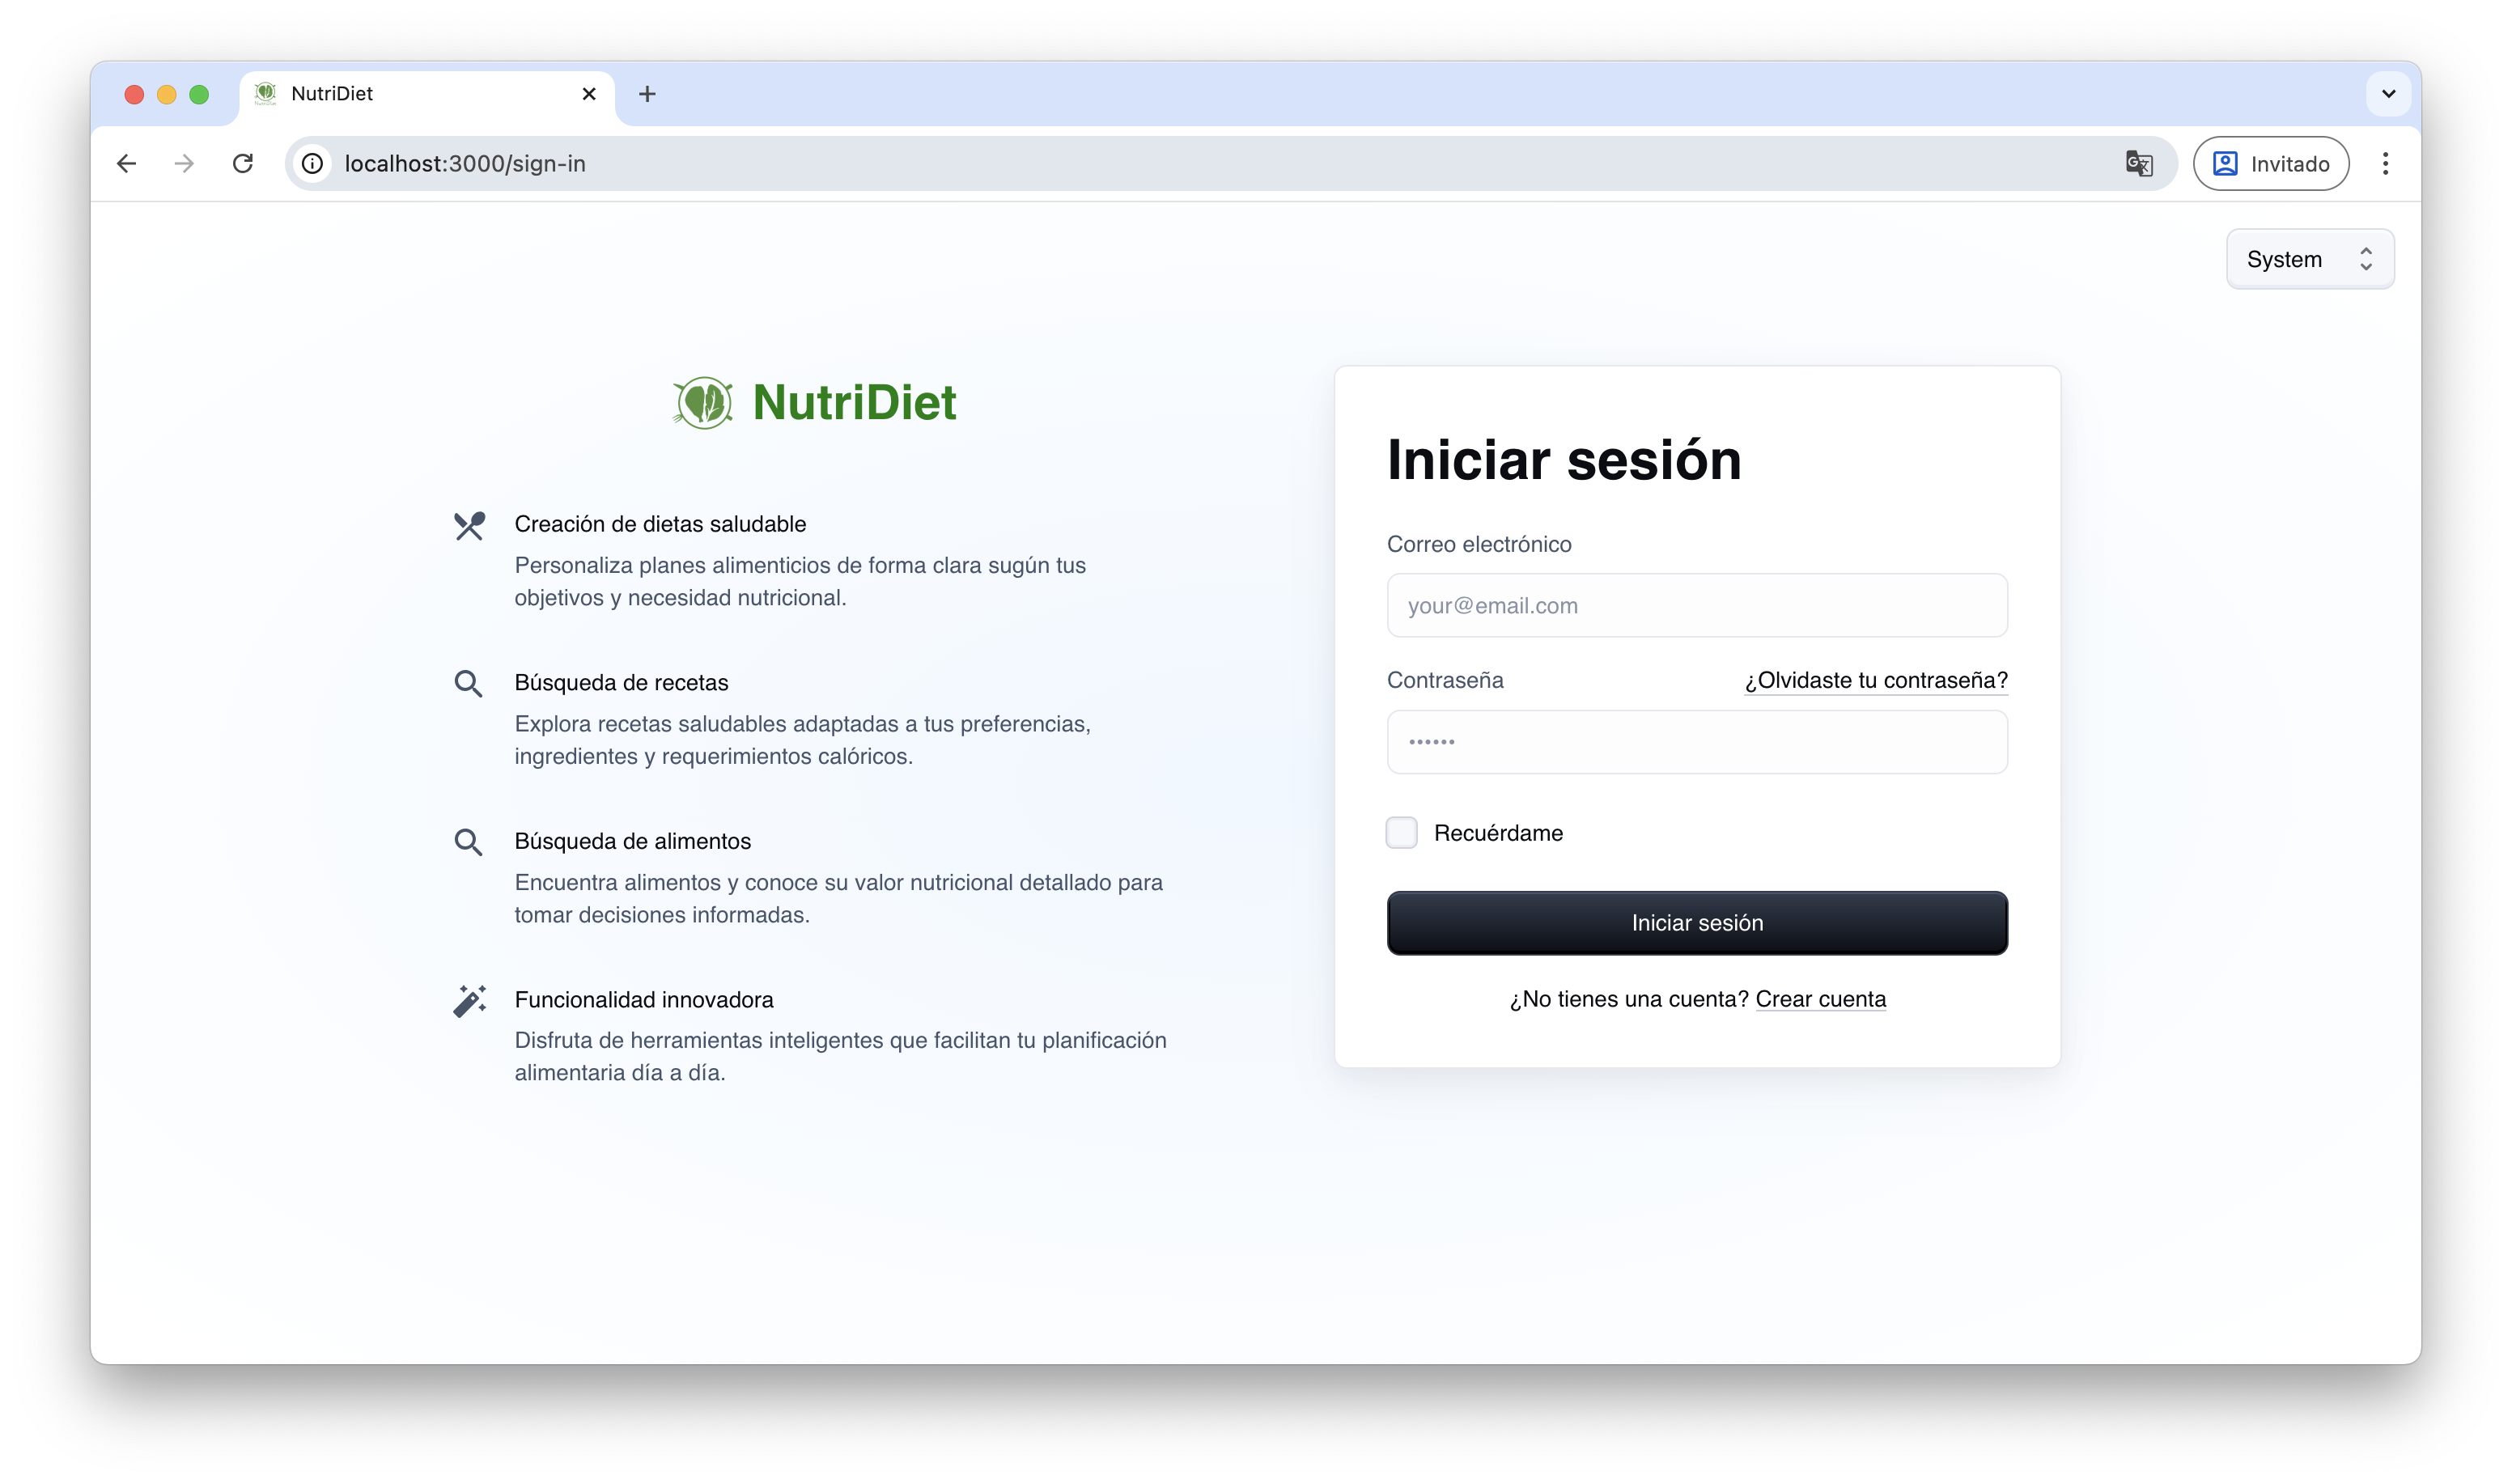
\includegraphics[width=1\linewidth]{Plantilla_TFG_latex//imagenes/Portada_web.png}
    \caption{Portada del sistema}
    \label{fig:Portada_web}
\end{figure}

\subsection{Registro}
Para comenzar a utilizar el sistema, el usuario debe acceder a la opción de registro (Crear cuenta, Figura~\ref{fig:Portada_web_registro}) y completar un formulario con su nombre completo, dirección de correo electrónico y una contraseña segura. Este paso es obligatorio para poder acceder a las funcionalidades del sistema.
\begin{figure}[H]
    \centering
    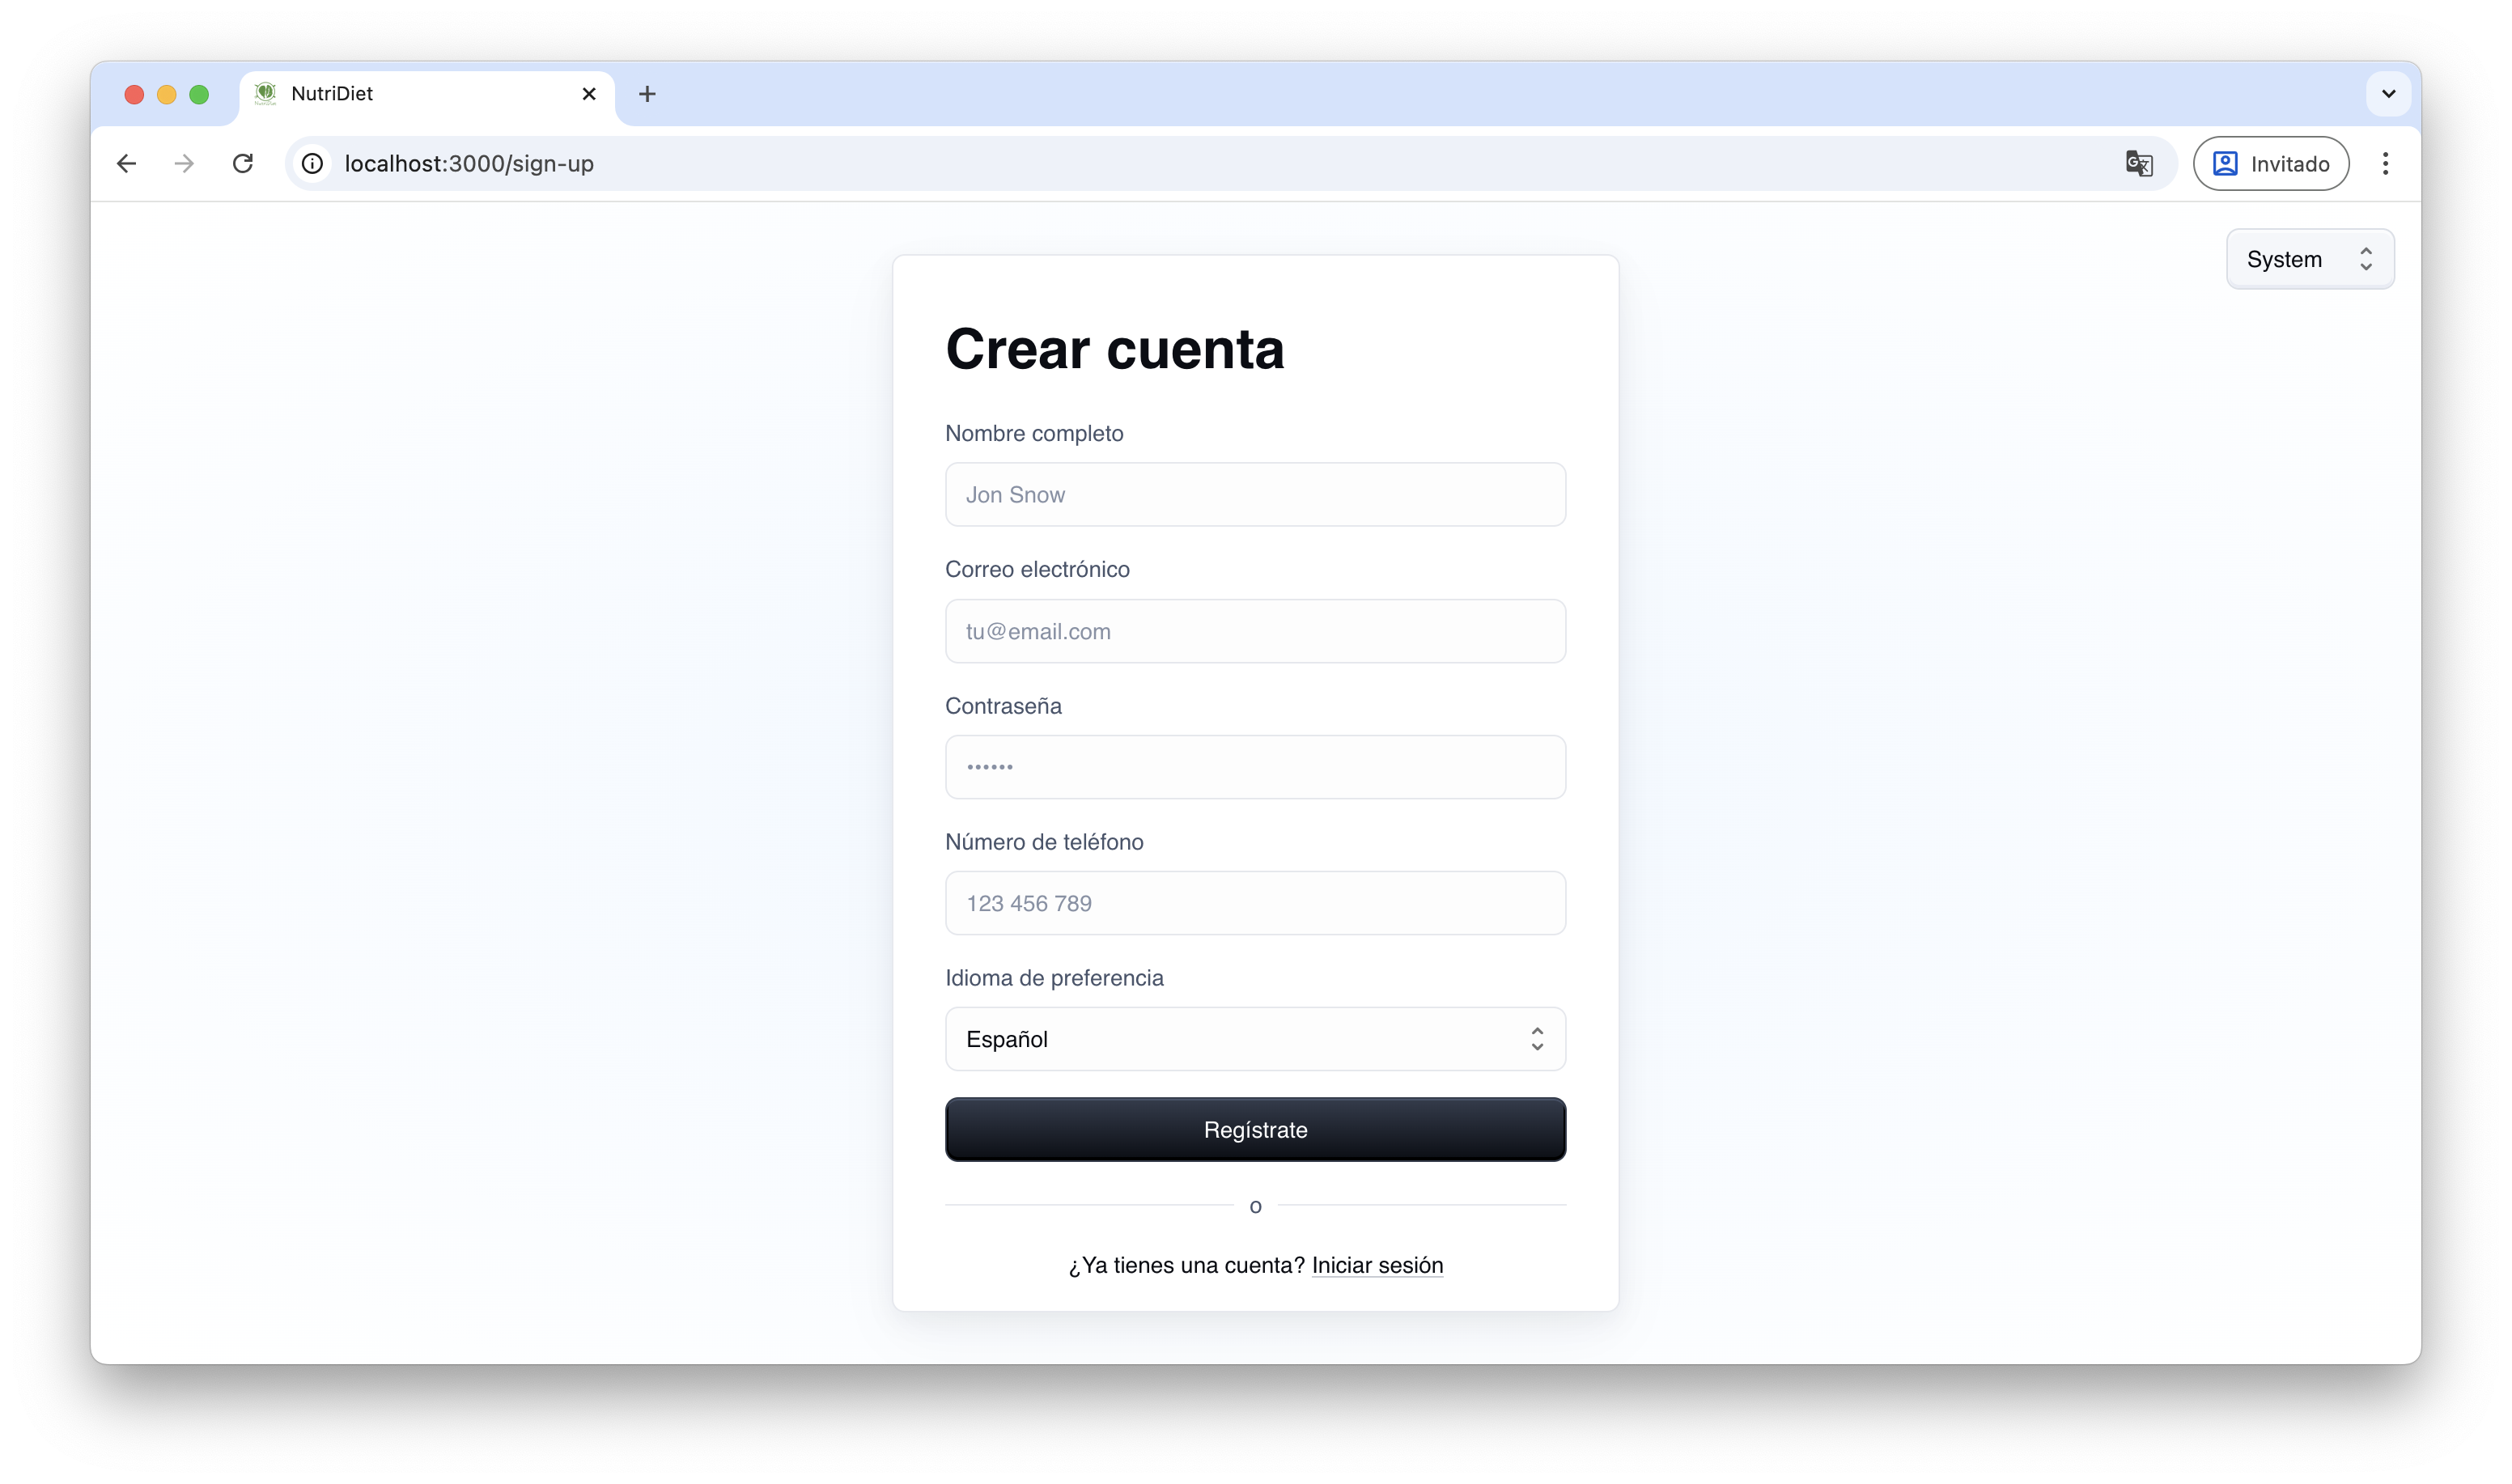
\includegraphics[width=1\linewidth]{Plantilla_TFG_latex//imagenes/Portada_web_registro.png}
    \caption{Tarjeta del registro}
    \label{fig:Portada_web_registro}
\end{figure}

\subsection{Inicio de sesión}
Una vez registrado, el usuario podrá iniciar sesión desde la pantalla principal ingresando su correo electrónico y contraseña. Si ha activado la opción de ``Recordar sesión", el sistema mantendrá su autenticación activa durante un periodo prolongado.

\subsection{Recuperación de contraseña}
En caso de olvidar la contraseña, el sistema dispone de un enlace para iniciar el proceso de recuperación mediante correo electrónico (Figura~\ref{fig:Portada_web_OContrasena}). No obstante, en esta versión, dicha funcionalidad está aún pendiente de implementación, por lo que se recomienda al usuario mantener sus credenciales a buen recaudo.
\begin{figure}[t]
    \centering
    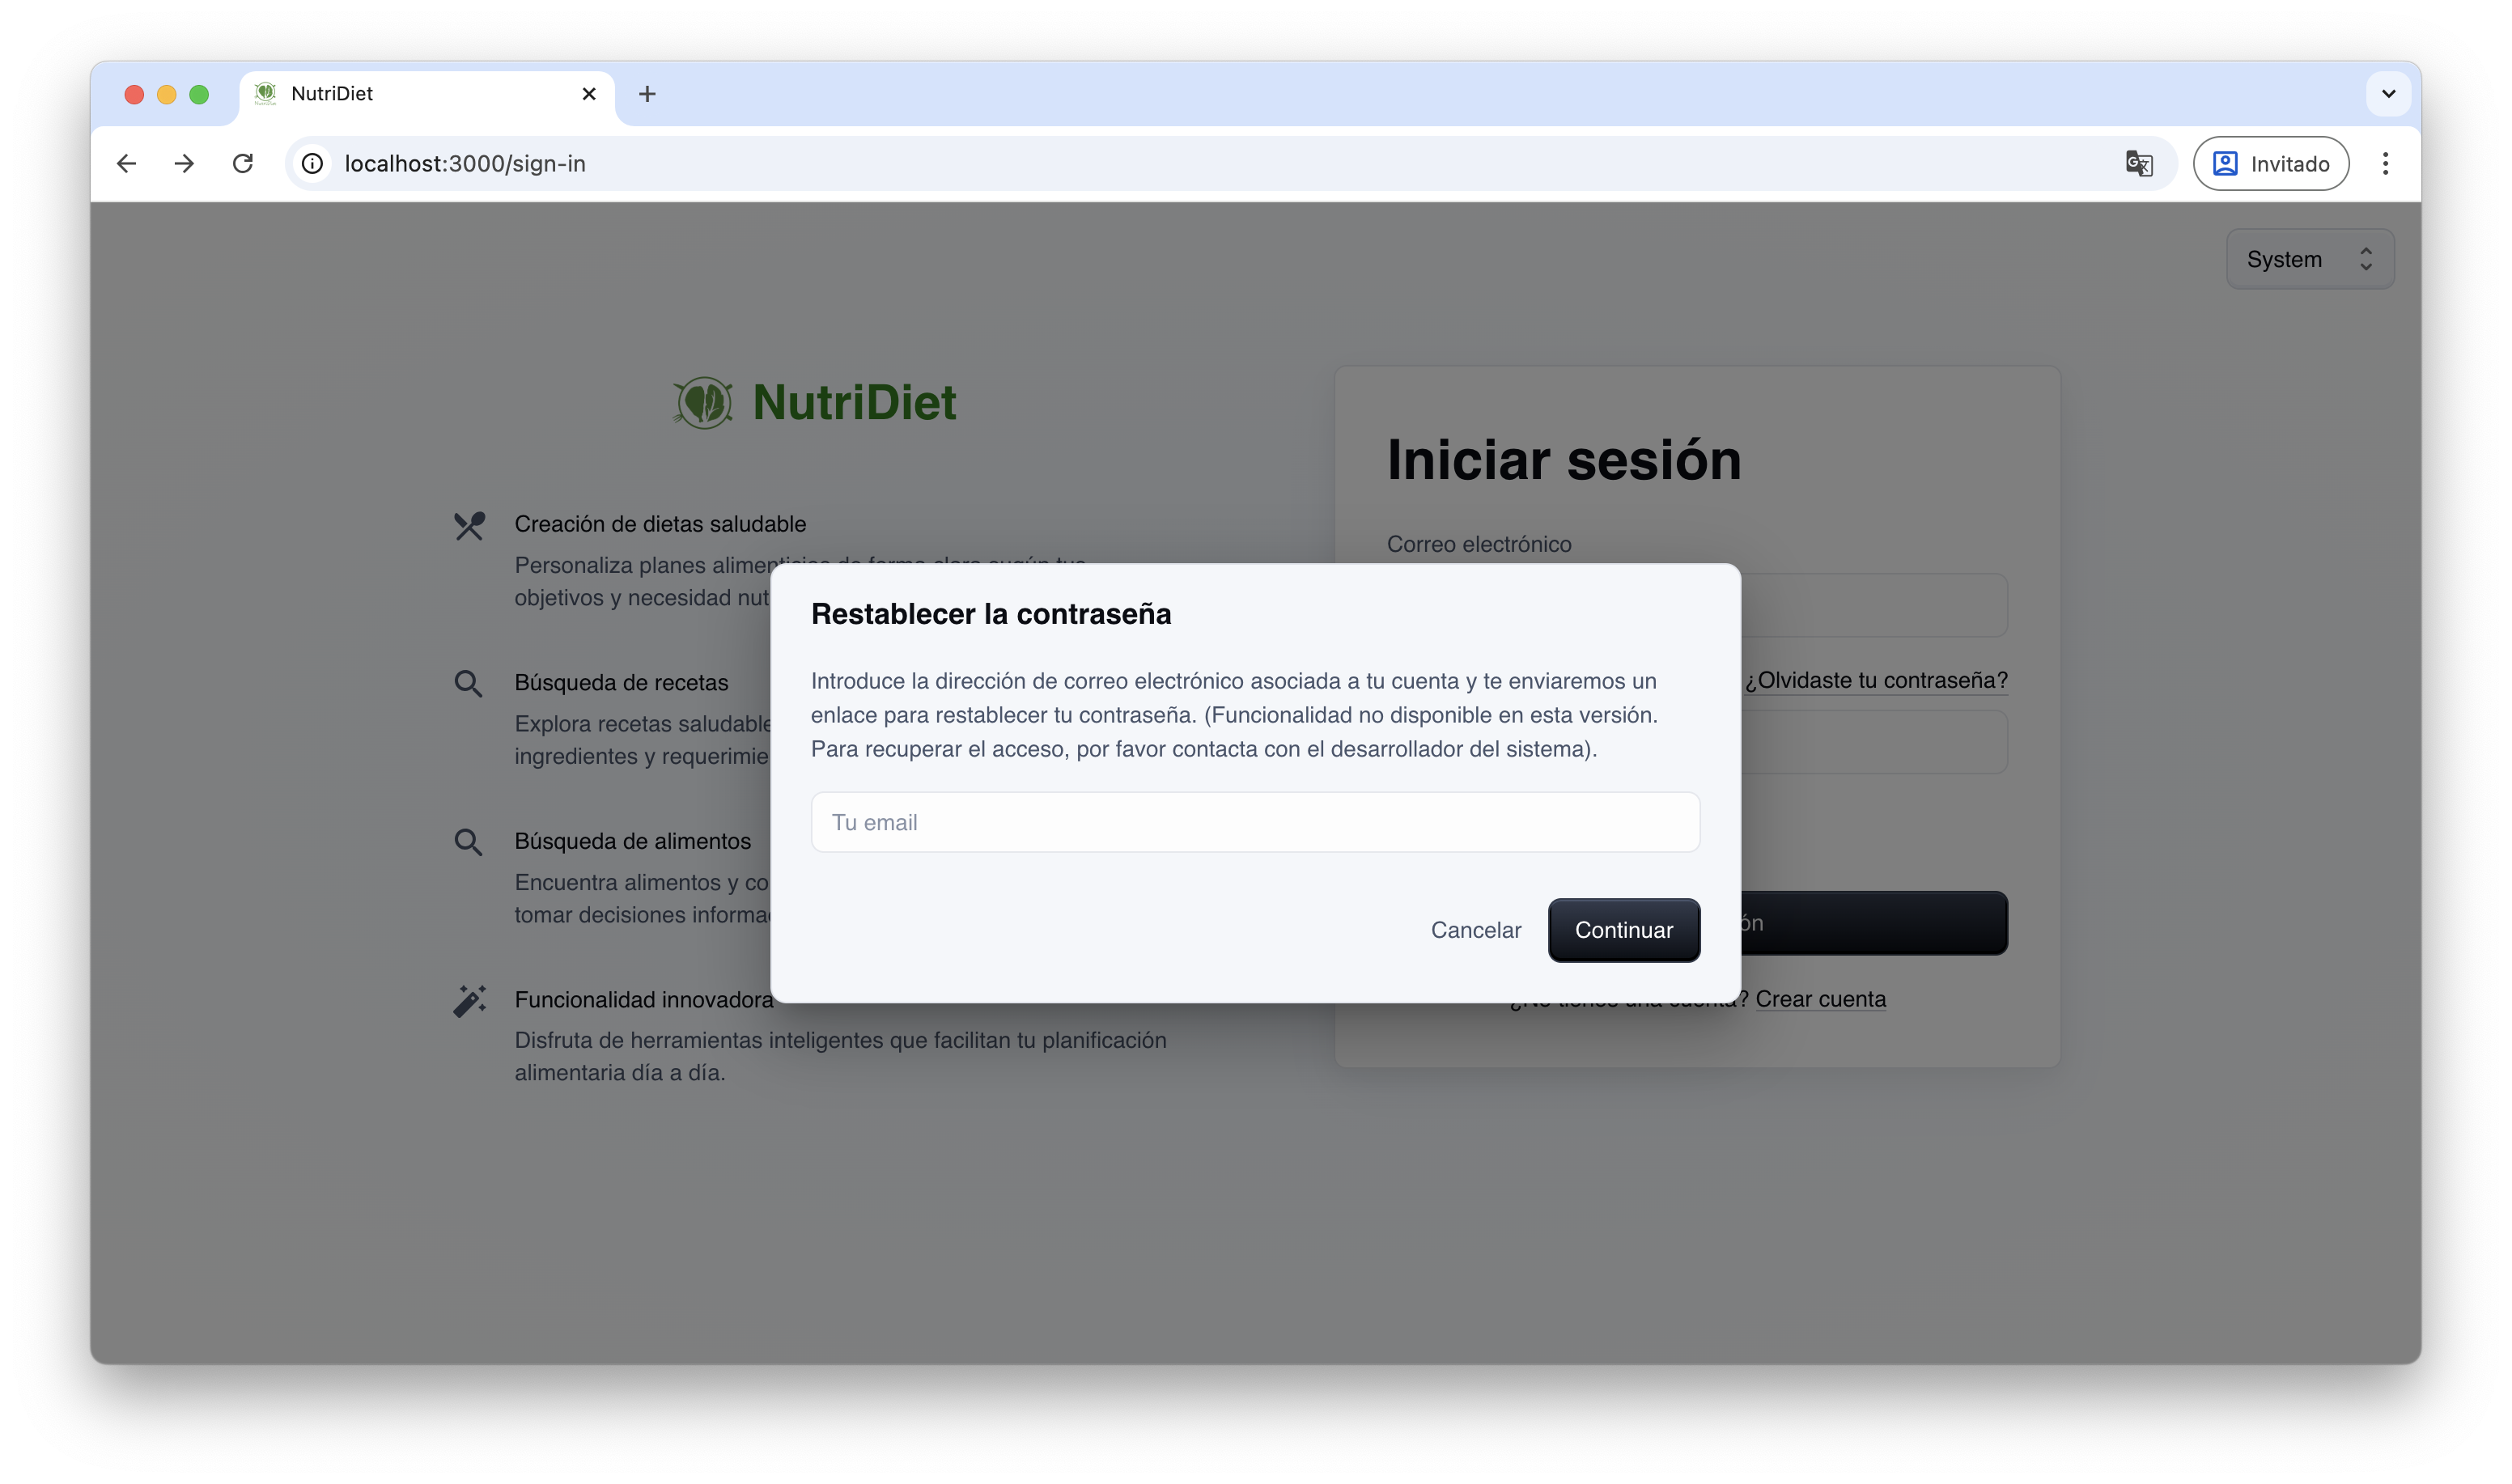
\includegraphics[width=1\linewidth]{Plantilla_TFG_latex//imagenes/Portada_web_OContrasena.png}
    \caption{Tarjeta de recuperación de contraseña}
    \label{fig:Portada_web_OContrasena}
\end{figure}

\section{Página de inicio}
La página de inicio (Figura~\ref{fig:pagina_inicio}) del sistema representa el primer punto de contacto para el usuario tras iniciar sesión. Desde esta interfaz se ofrece una visión general de las funcionalidades disponibles y se proporciona acceso rápido a los módulos principales del sistema.

La estructura de la página de inicio está diseñada para maximizar la usabilidad y facilitar la navegación. Entre sus componentes se encuentran:

\begin{itemize}
    \item Barra de navegación lateral: permite acceder a las secciones clave del sistema, como pacientes, recetas, ingestas y dietas.
    
    \item Cabecera del sistema: contiene un rastro de navegación (``breadcrumb''), el perfil del usuario, representado mediante un avatar generado dinámicamente, y un menú de opciones desplegable accesible desde dicho avatar.

    \item Tarjetas informativas: destacan las funcionalidades principales mediante iconos y descripciones breves, como “Crear nueva dieta”, “Buscar receta” o “Registrar paciente”.
    
\end{itemize}

\begin{figure}[t]
    \centering
    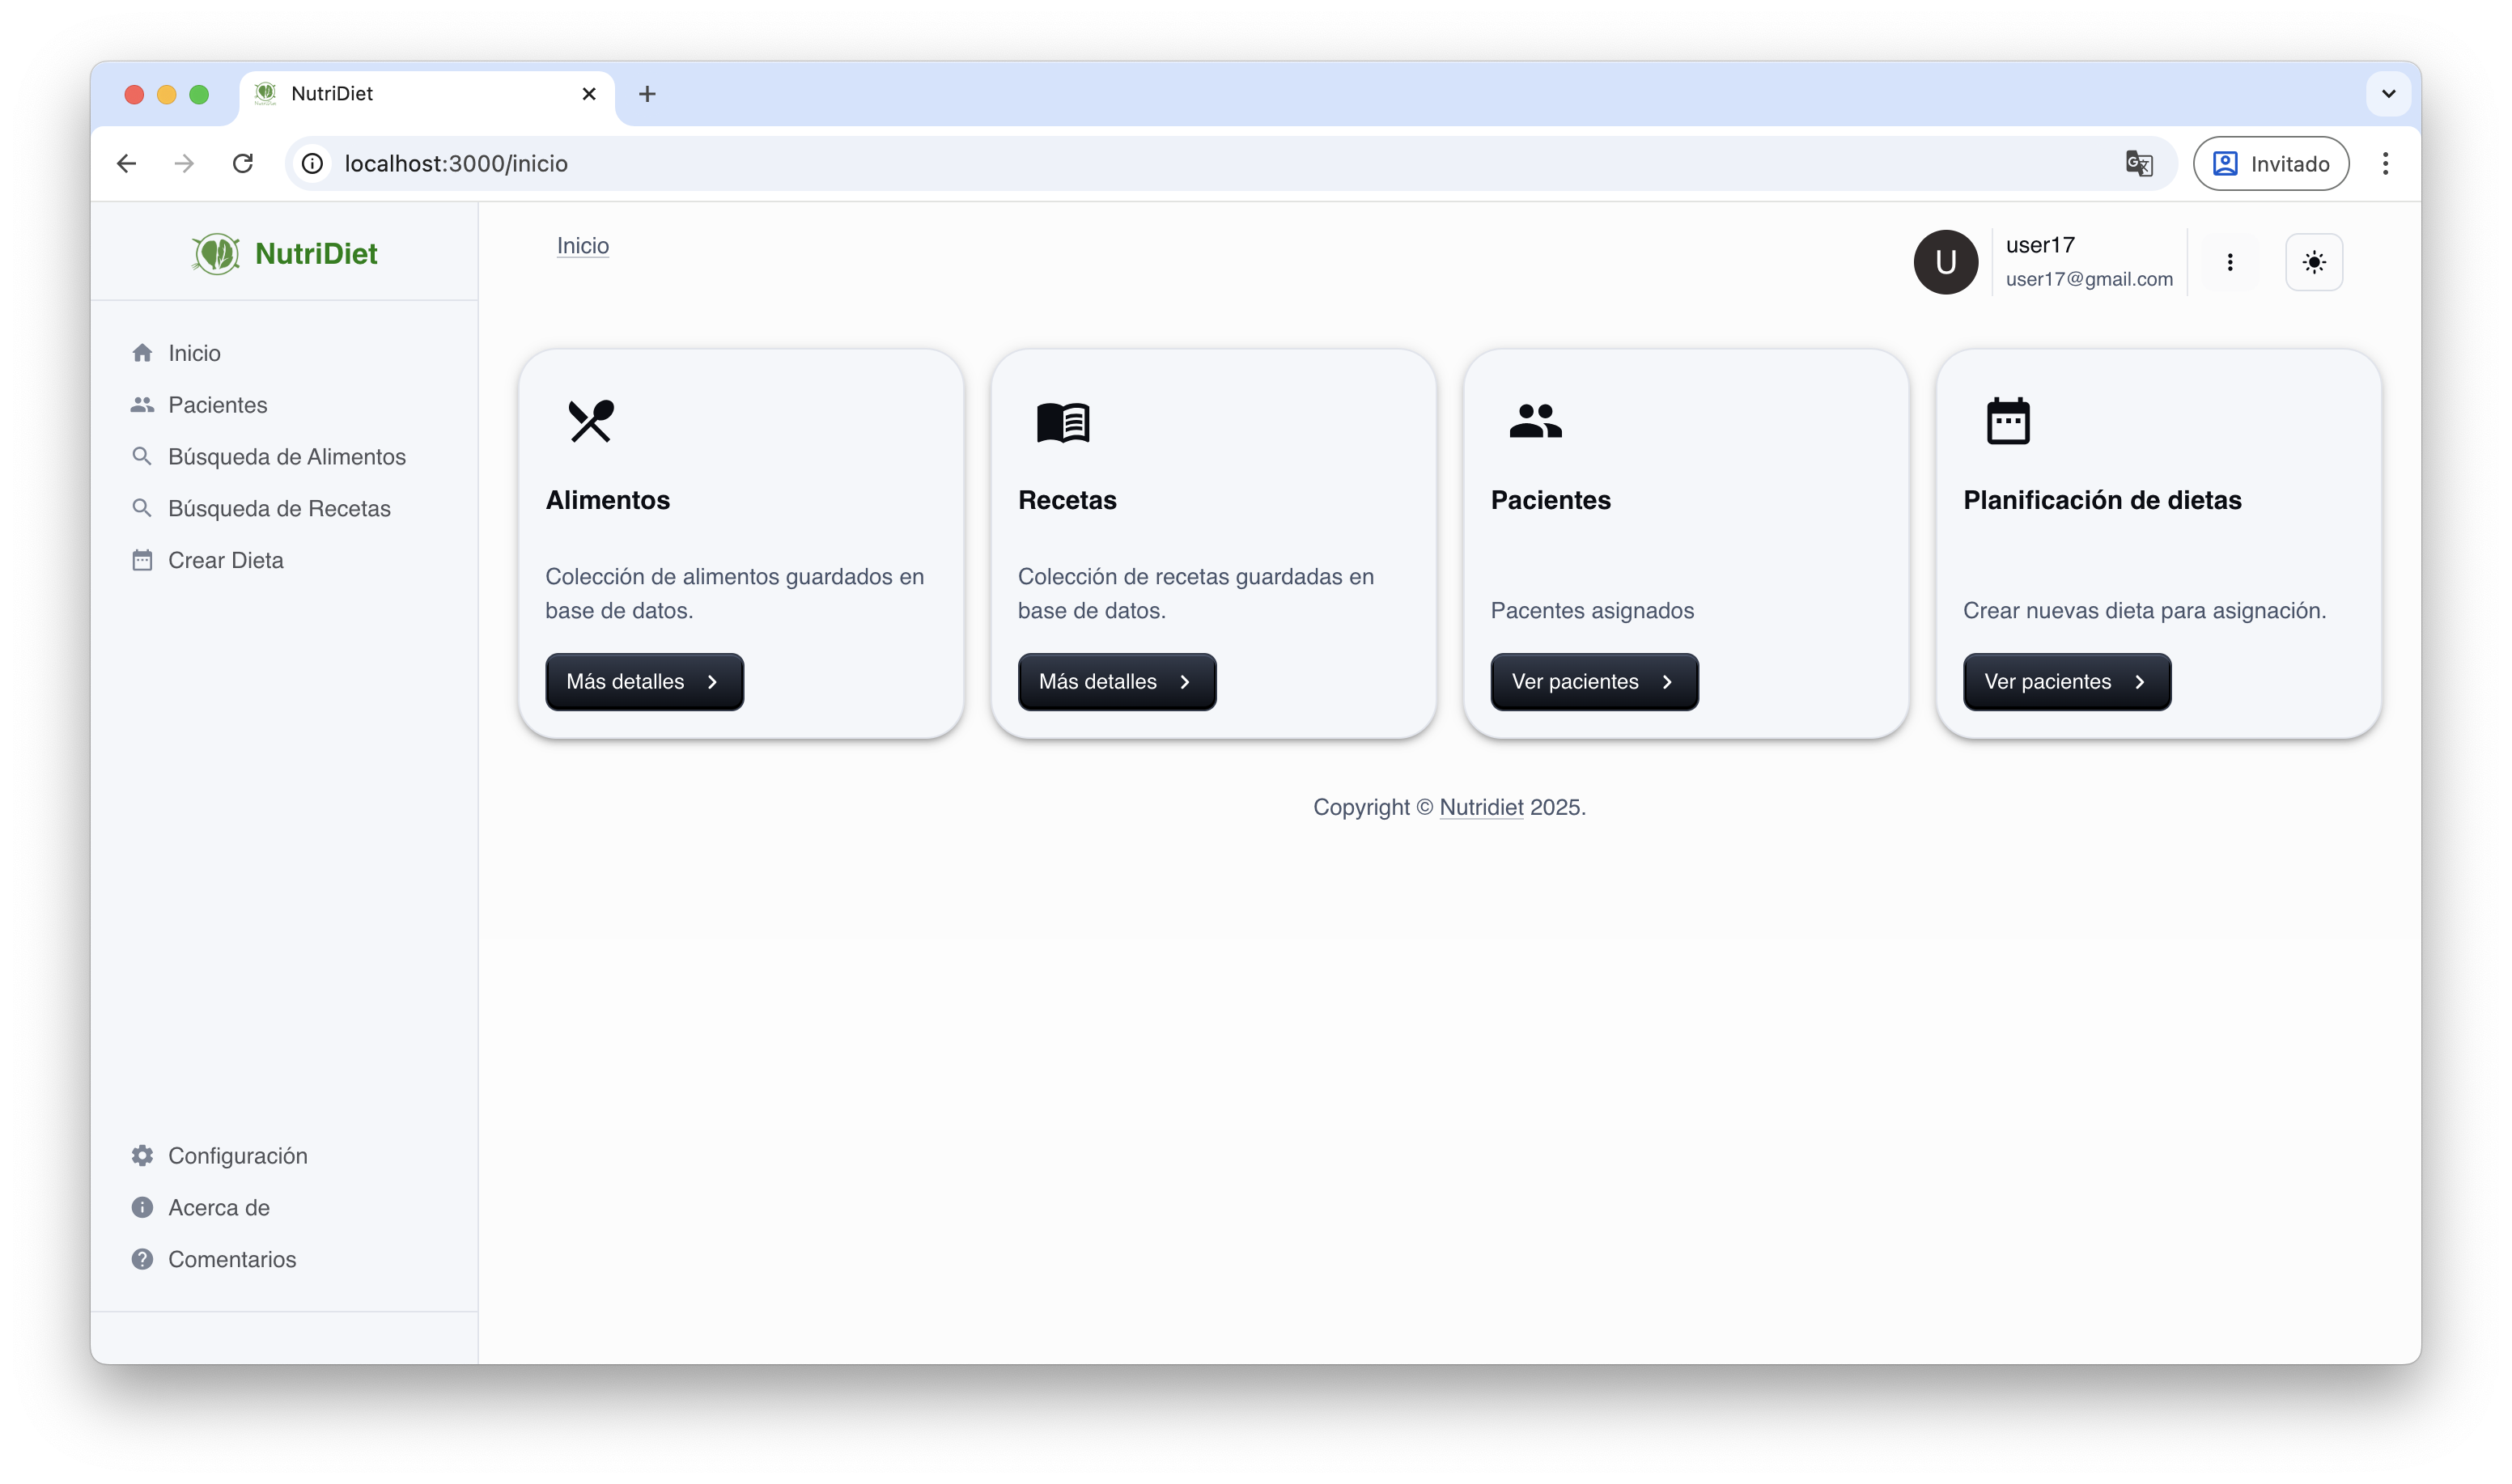
\includegraphics[width=1\linewidth]{Plantilla_TFG_latex/imagenes/PagInicio.png}
    \caption{Interfaz de la página de inicio tras iniciar sesión}
    \label{fig:pagina_inicio}
\end{figure}

\subsection{Menú de opciones del Usuario}
Muestra un avatar generado automáticamente a partir de las iniciales del nombre del usuario, acompañado por su nombre completo y dirección de correo electrónico (Figura~\ref{fig:PagInicio_menuO}). Al hacer clic en el icono de tres puntos junto al avatar, se despliega un menú de opciones que permite realizar acciones como acceder al perfil, modificar configuraciones de la cuenta o cerrar sesión.
\begin{figure}
    \centering
    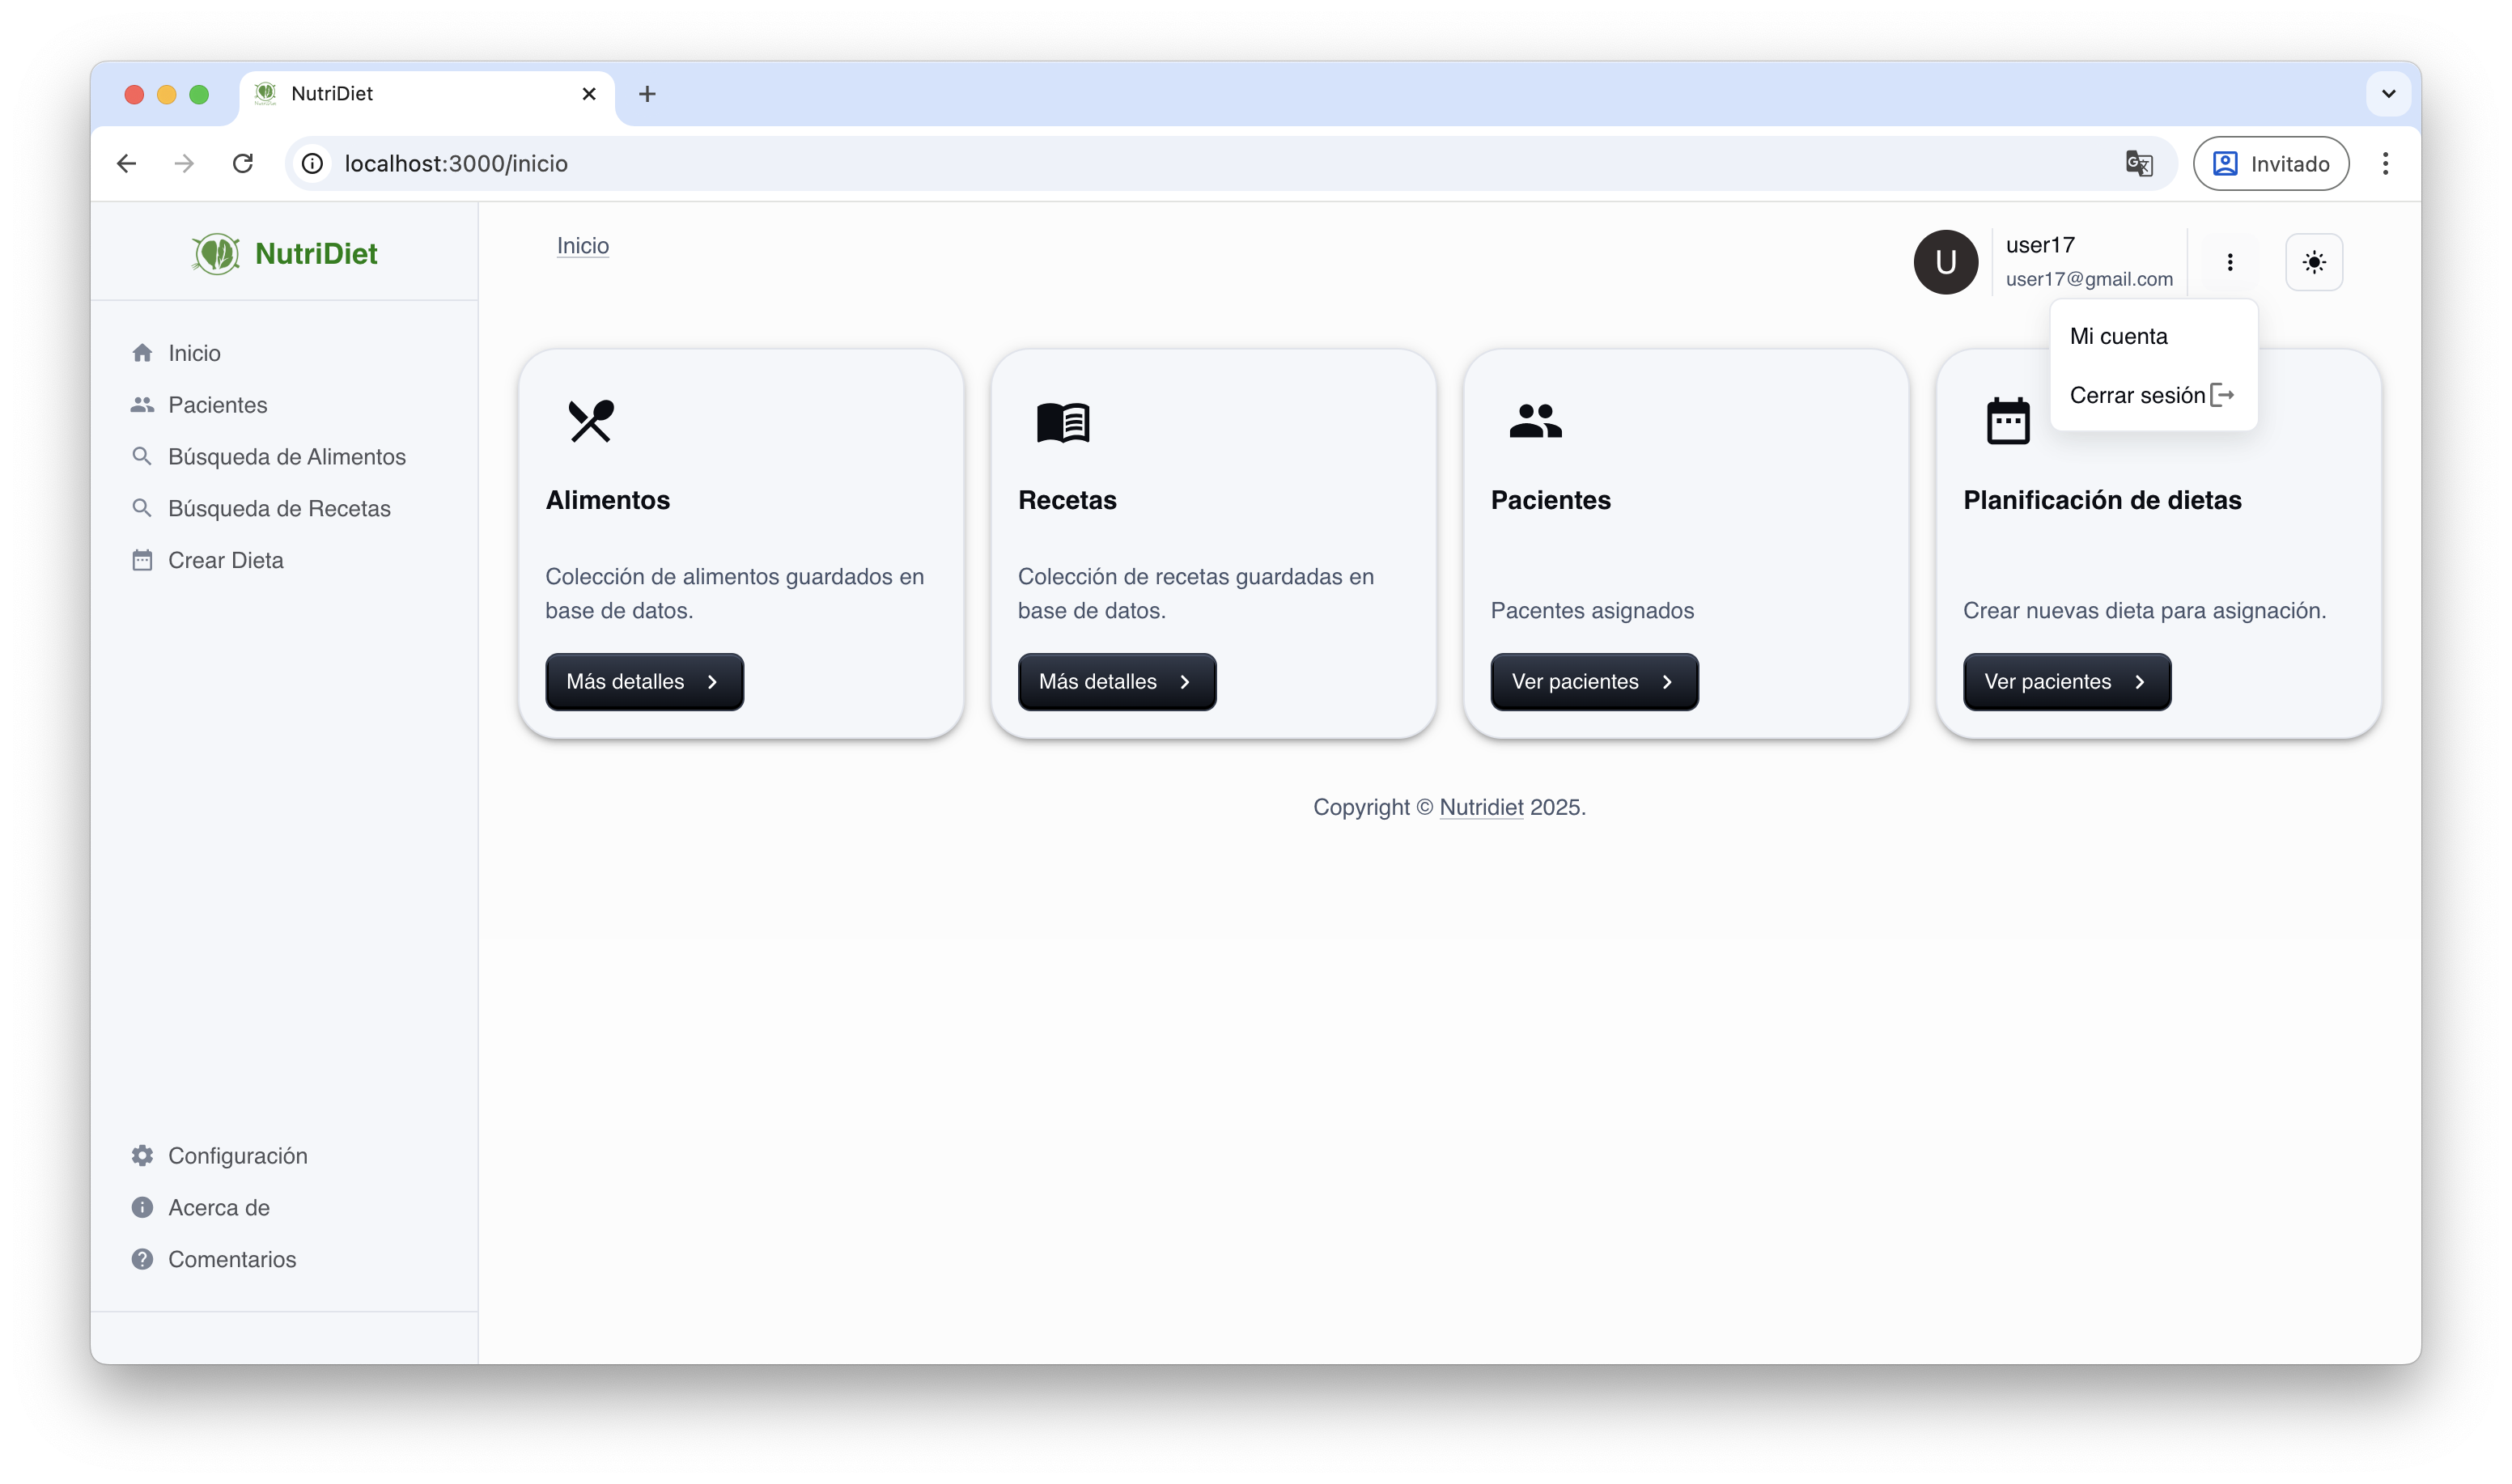
\includegraphics[width=1\linewidth]{Plantilla_TFG_latex/imagenes/PagInicio_OM.png}
    \caption{Menú de opciones del Usuario}
    \label{fig:PagInicio_menuO}
\end{figure}

\subsubsection{Mi cuenta}
Esta página (Figura~\ref{fig:PagInicio_MiCuenta}) permite al usuario gestionar y actualizar su información personal de forma segura. El usuario puede modificar datos como el nombre completo, el número de teléfono y el idioma de preferencias.

Además, se incluye una opción para cambiar la contraseña, lo que refuerza la seguridad y permite mantener actualizadas las credenciales de acceso.

\begin{figure}
    \centering
    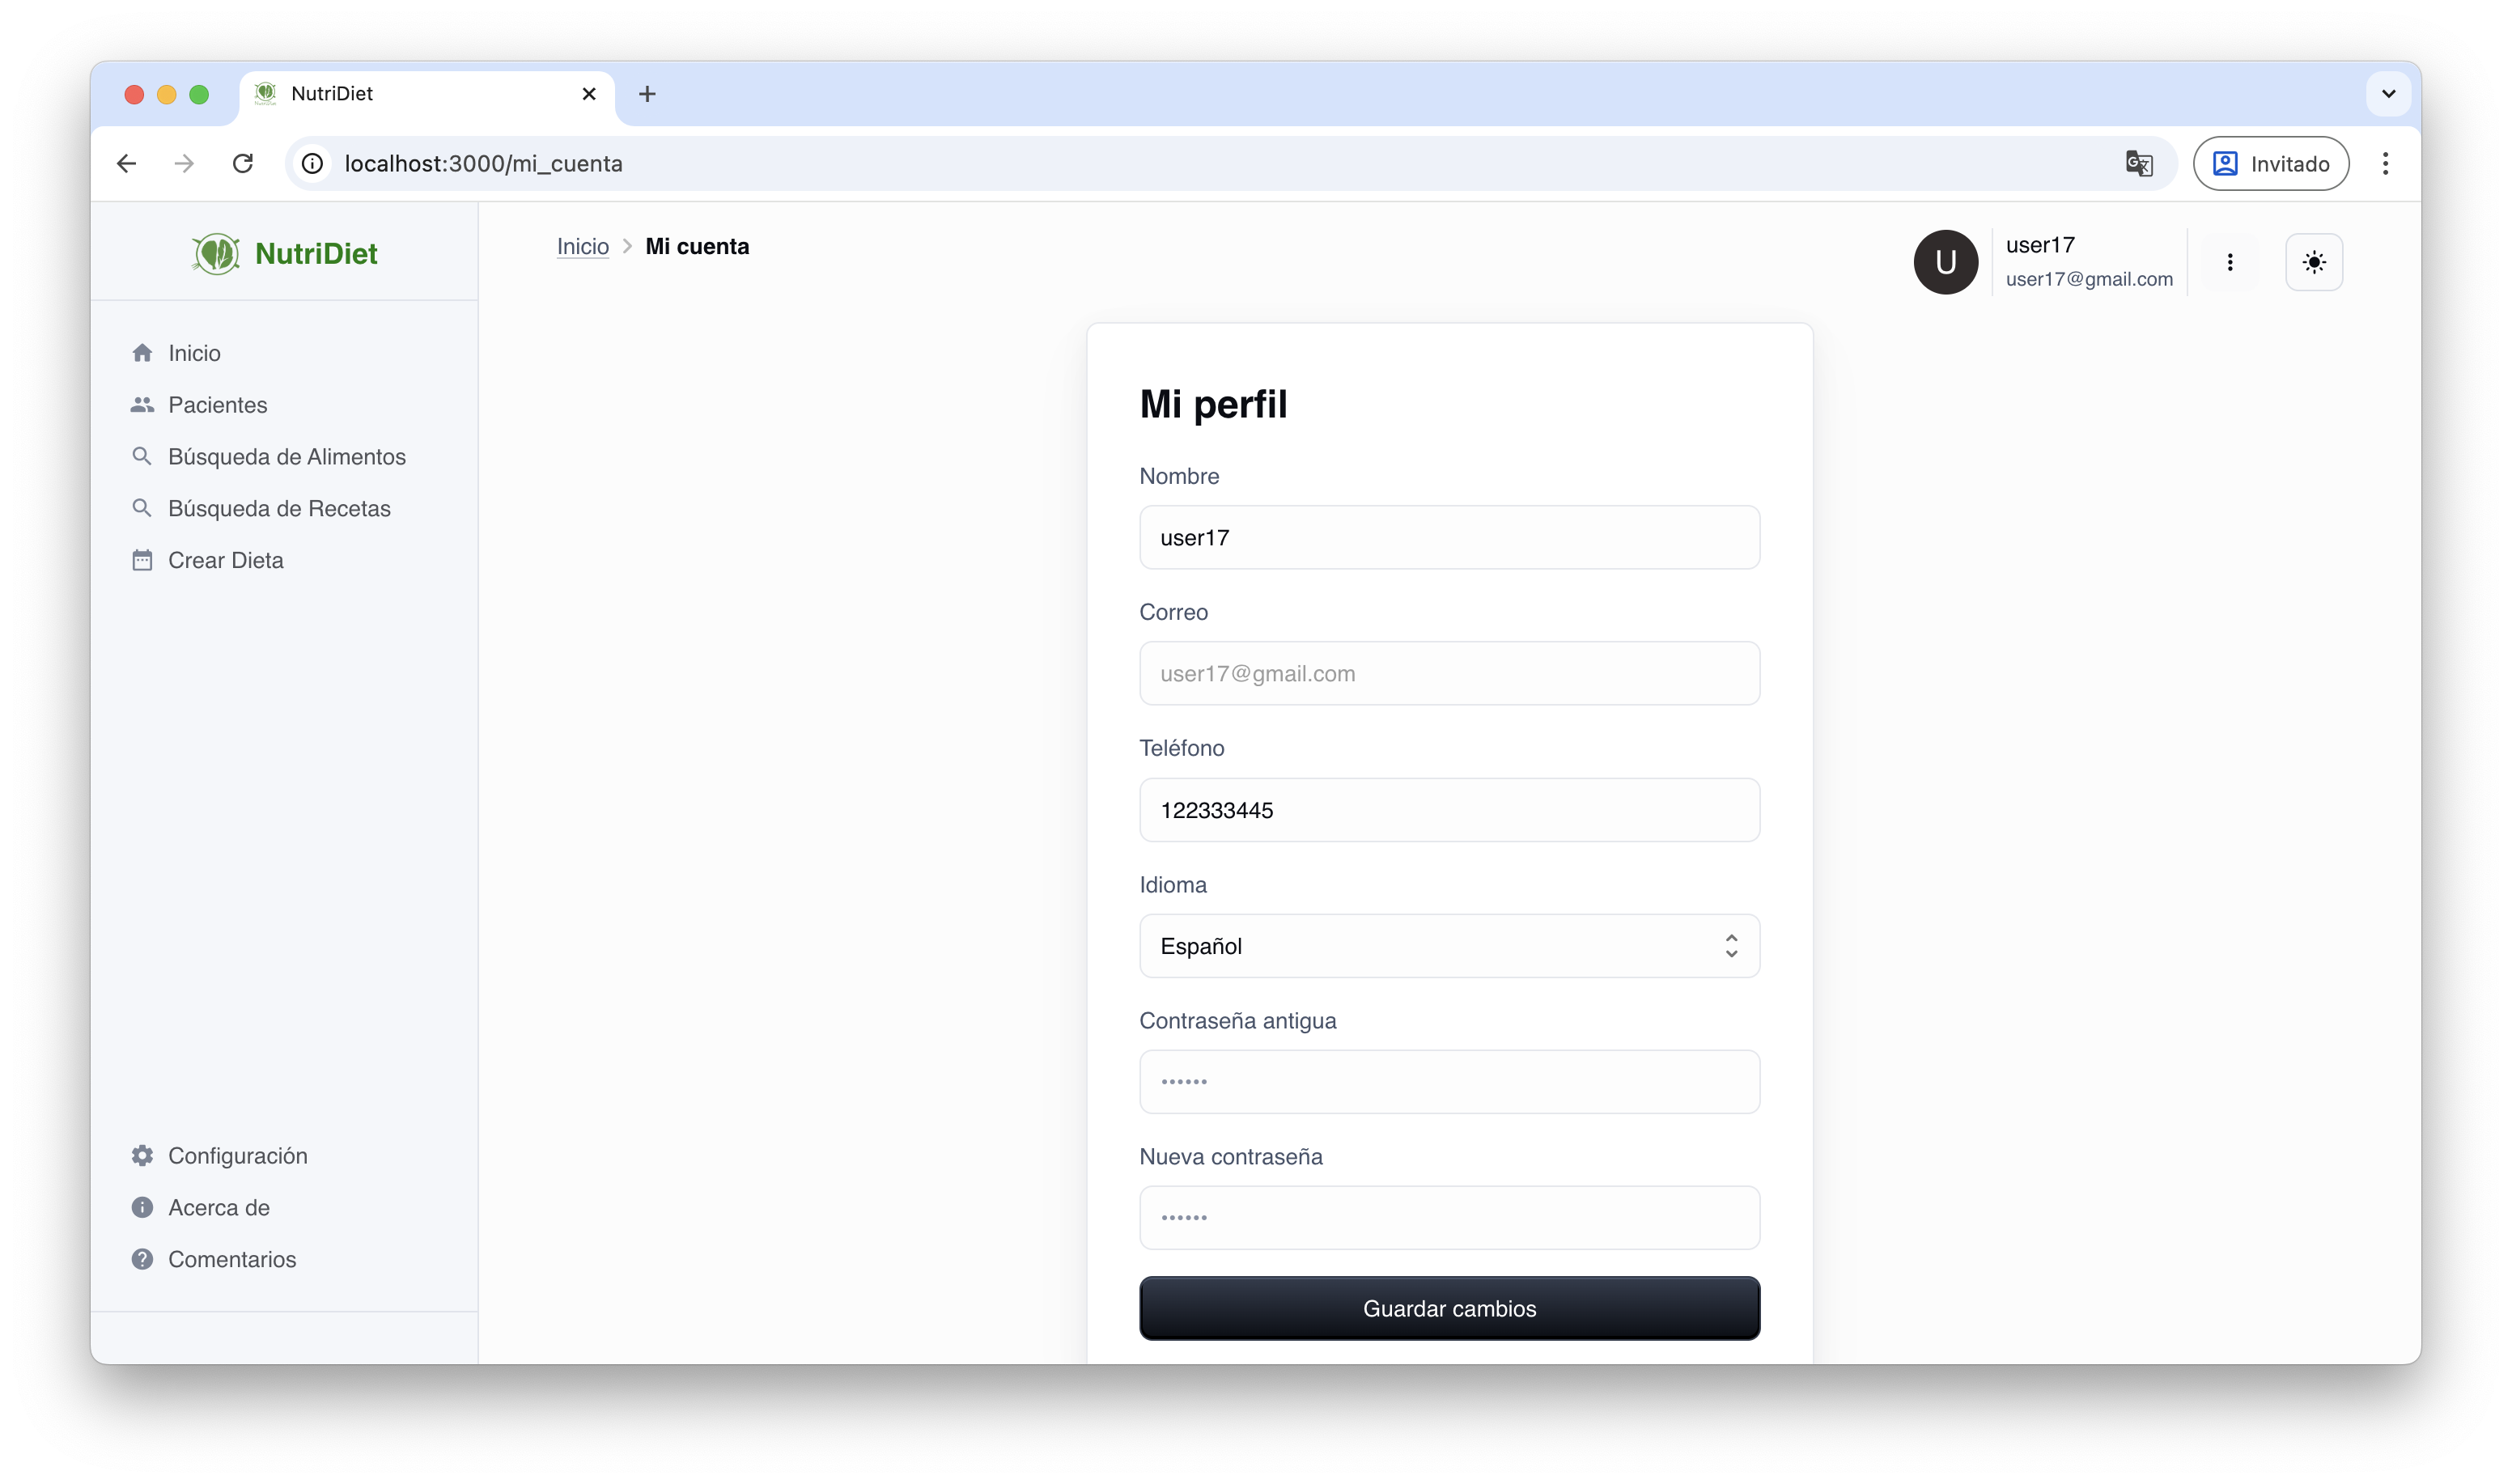
\includegraphics[width=1\linewidth]{Plantilla_TFG_latex/imagenes/PagInicio_MiCuenta.png}
    \caption{Vista de gestión de cuenta del usuario}
    \label{fig:PagInicio_MiCuenta}
\end{figure}

\subsubsection{Cerrar sesión}

El sistema permite al usuario cerrar sesión de forma segura mediante el menú de opciones accesible desde el avatar situado en la cabecera. Al seleccionar la opción Cerrar sesión, la sesión actual se finaliza y el usuario es redirigido automáticamente a la portada del sistema, donde podrá iniciar sesión nuevamente o registrar una nueva cuenta.

\section{Gestión de pacientes}

La sección de gestión de pacientes (Figura~\ref{fig:PagPaciente_ini}) permite al usuario registrar, visualizar, editar y eliminar pacientes asociados a su cuenta profesional. Se ha diseñado teniendo en cuenta que la aplicación está dirigida a personal experto, esta funcionalidad resulta esencial para organizar y personalizar el seguimiento clínico de cada caso.

\begin{itemize}
    \item Añadir paciente: Tarjeta visible en la interfaz principal que permite iniciar el proceso de registro de un nuevo paciente. Al hacer clic, se despliega un formulario de creación.
    
    \item Tarjeta paciente: Tarjeta que representa individualmente a cada paciente. Muestra su información básica y proporciona botones para editar o eliminar al paciente.

    \item Visualización de detalle de dieta: Desde cada tarjeta de paciente, el usuario puede acceder a las dietas previamente asignadas. 
    
    \item Navegación paginada: Si hay más de cinco pacientes, se activa una navegación por páginas, que permite avanzar o retroceder en bloques de cinco registros.
\end{itemize}

\begin{figure}[H]
    \centering
    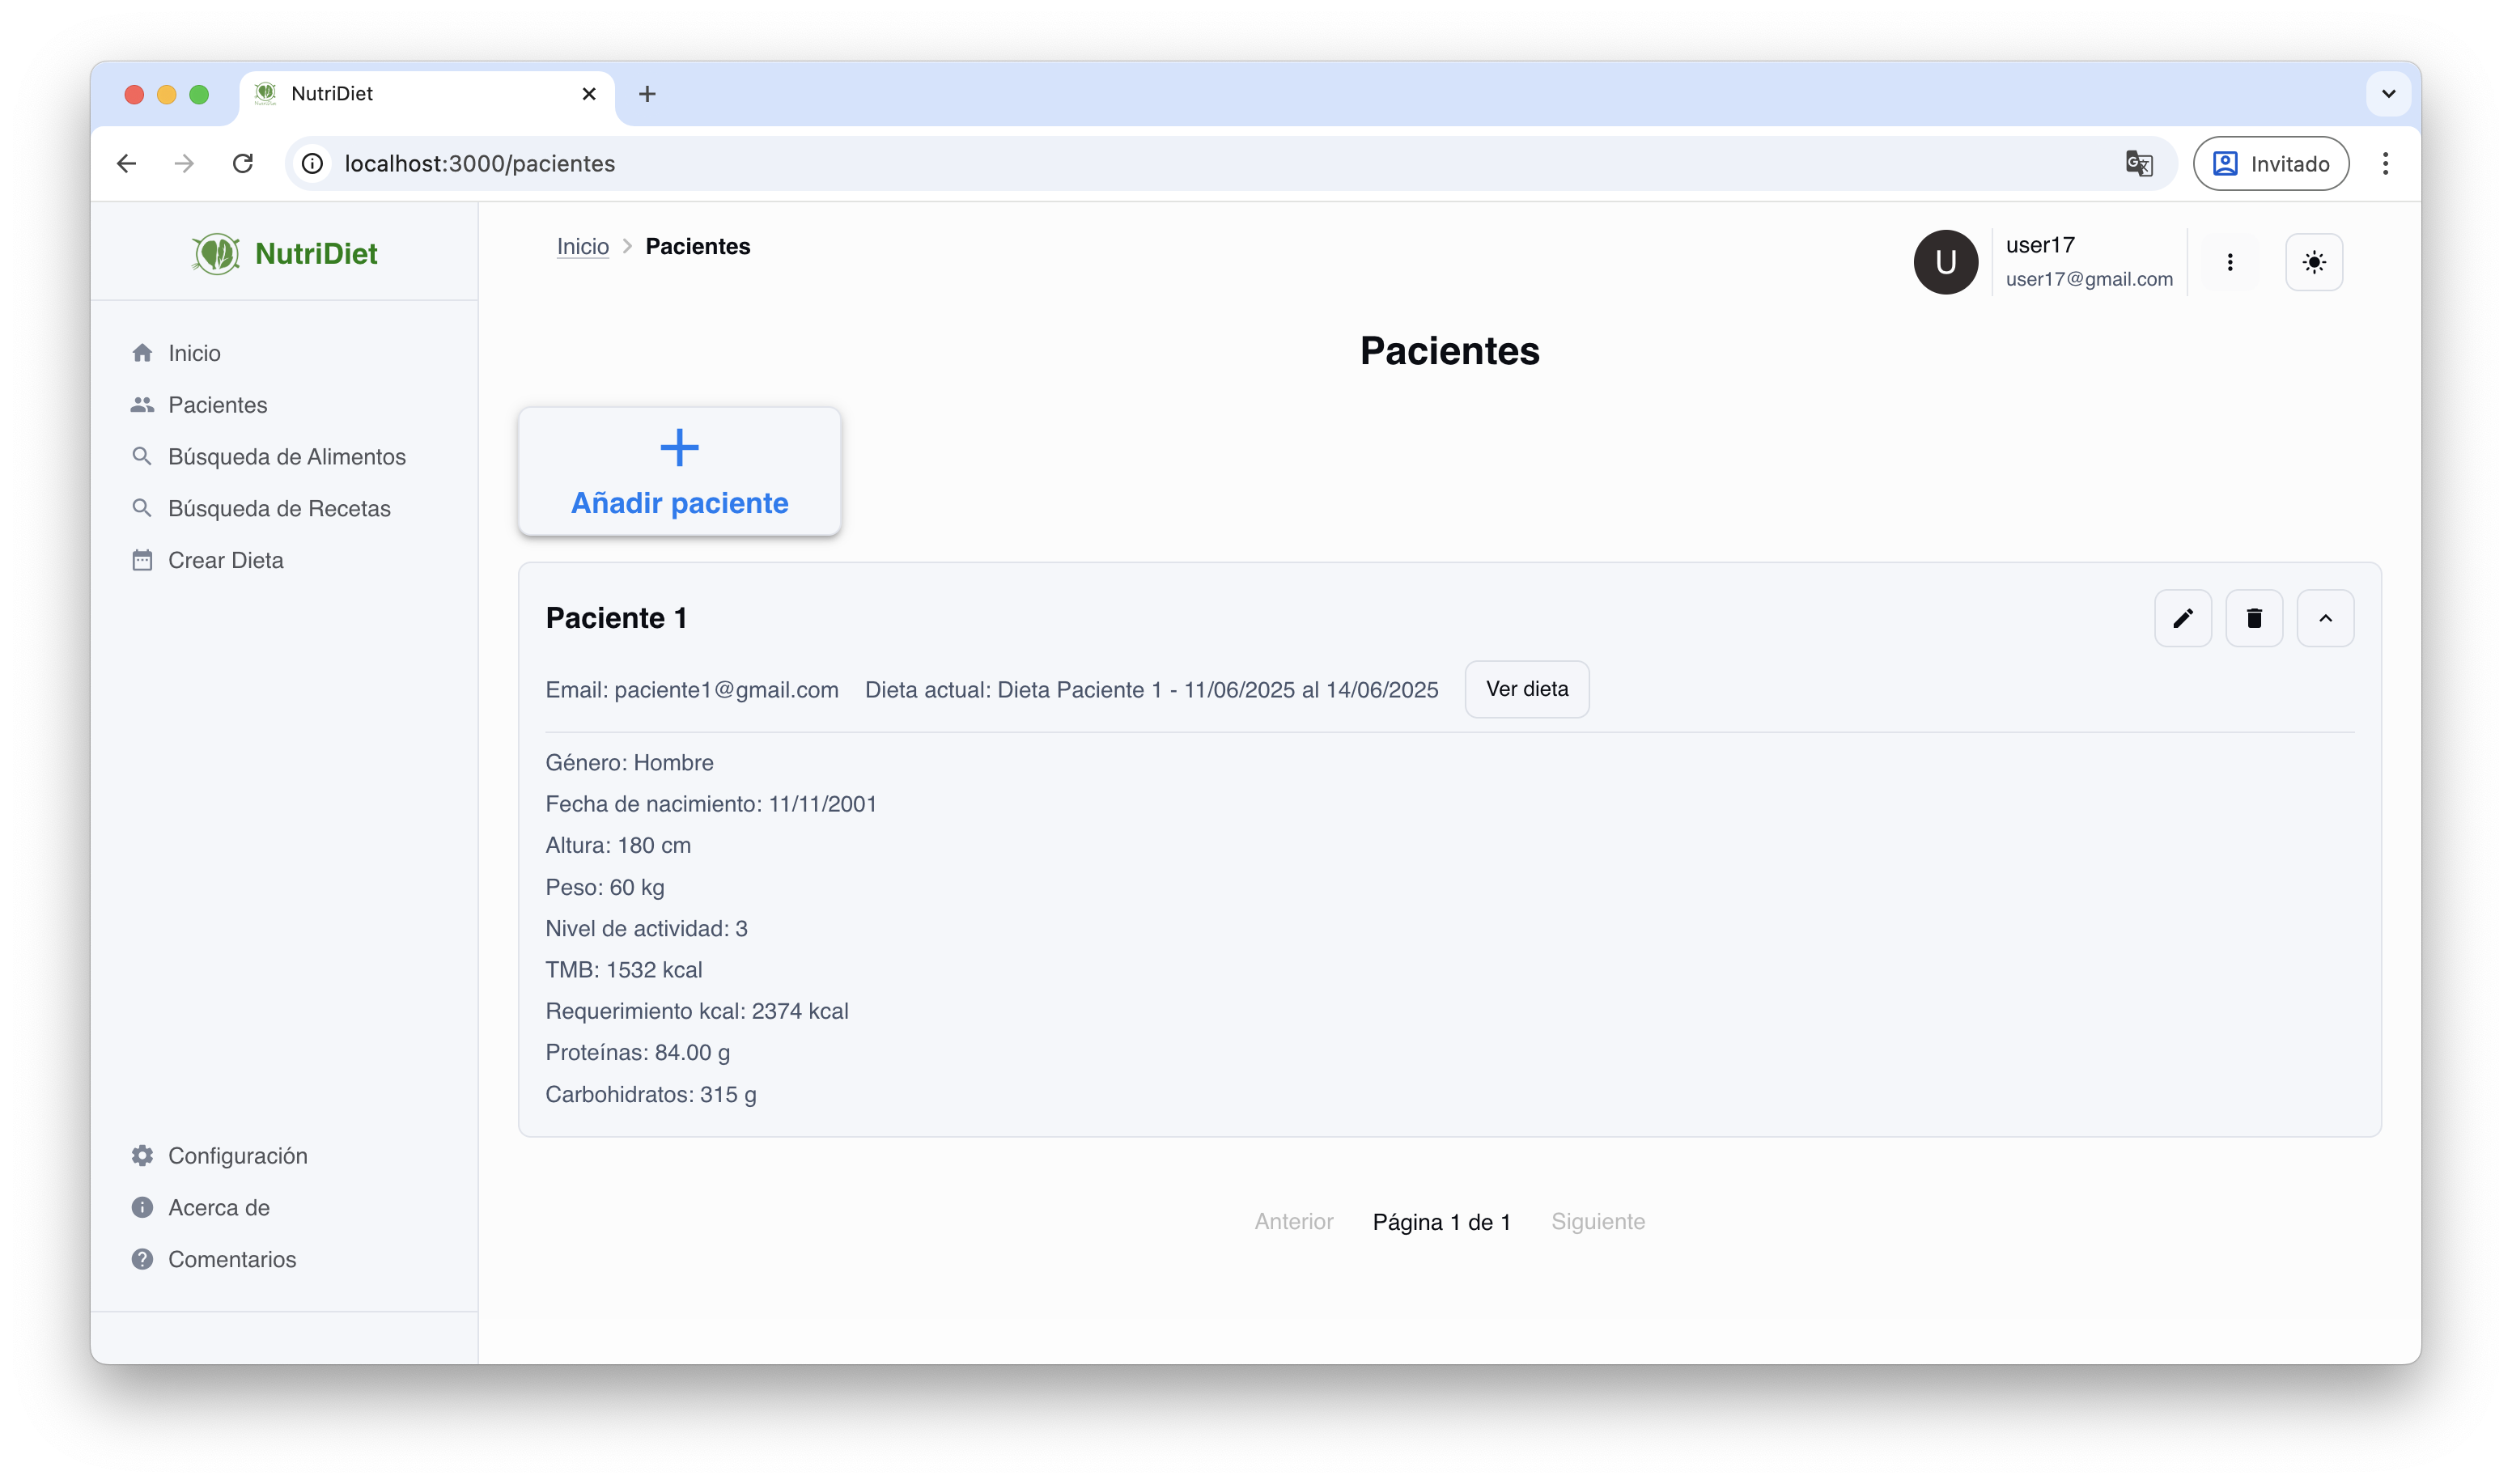
\includegraphics[width=1\linewidth]{Plantilla_TFG_latex/imagenes/PagPaciente_ini.png}
    \caption{Vista de Pacientes}
    \label{fig:PagPaciente_ini}
\end{figure}

\subsection{Añadir paciente}
Para registrar nuevos pacientes se realiza mediante este formulario accesible desde la interfaz principal de la sección Pacientes (Figura~\ref{fig:Paciente_crearP}). Una vez completado el formulario, pulsar el botón ``Guardar'' para registrar al paciente en la base de datos. Al finalizar, el paciente aparecerá automáticamente en el listado general, y podrá ser editado o eliminado posteriormente si es necesario.

\begin{figure}[H]
    \centering
    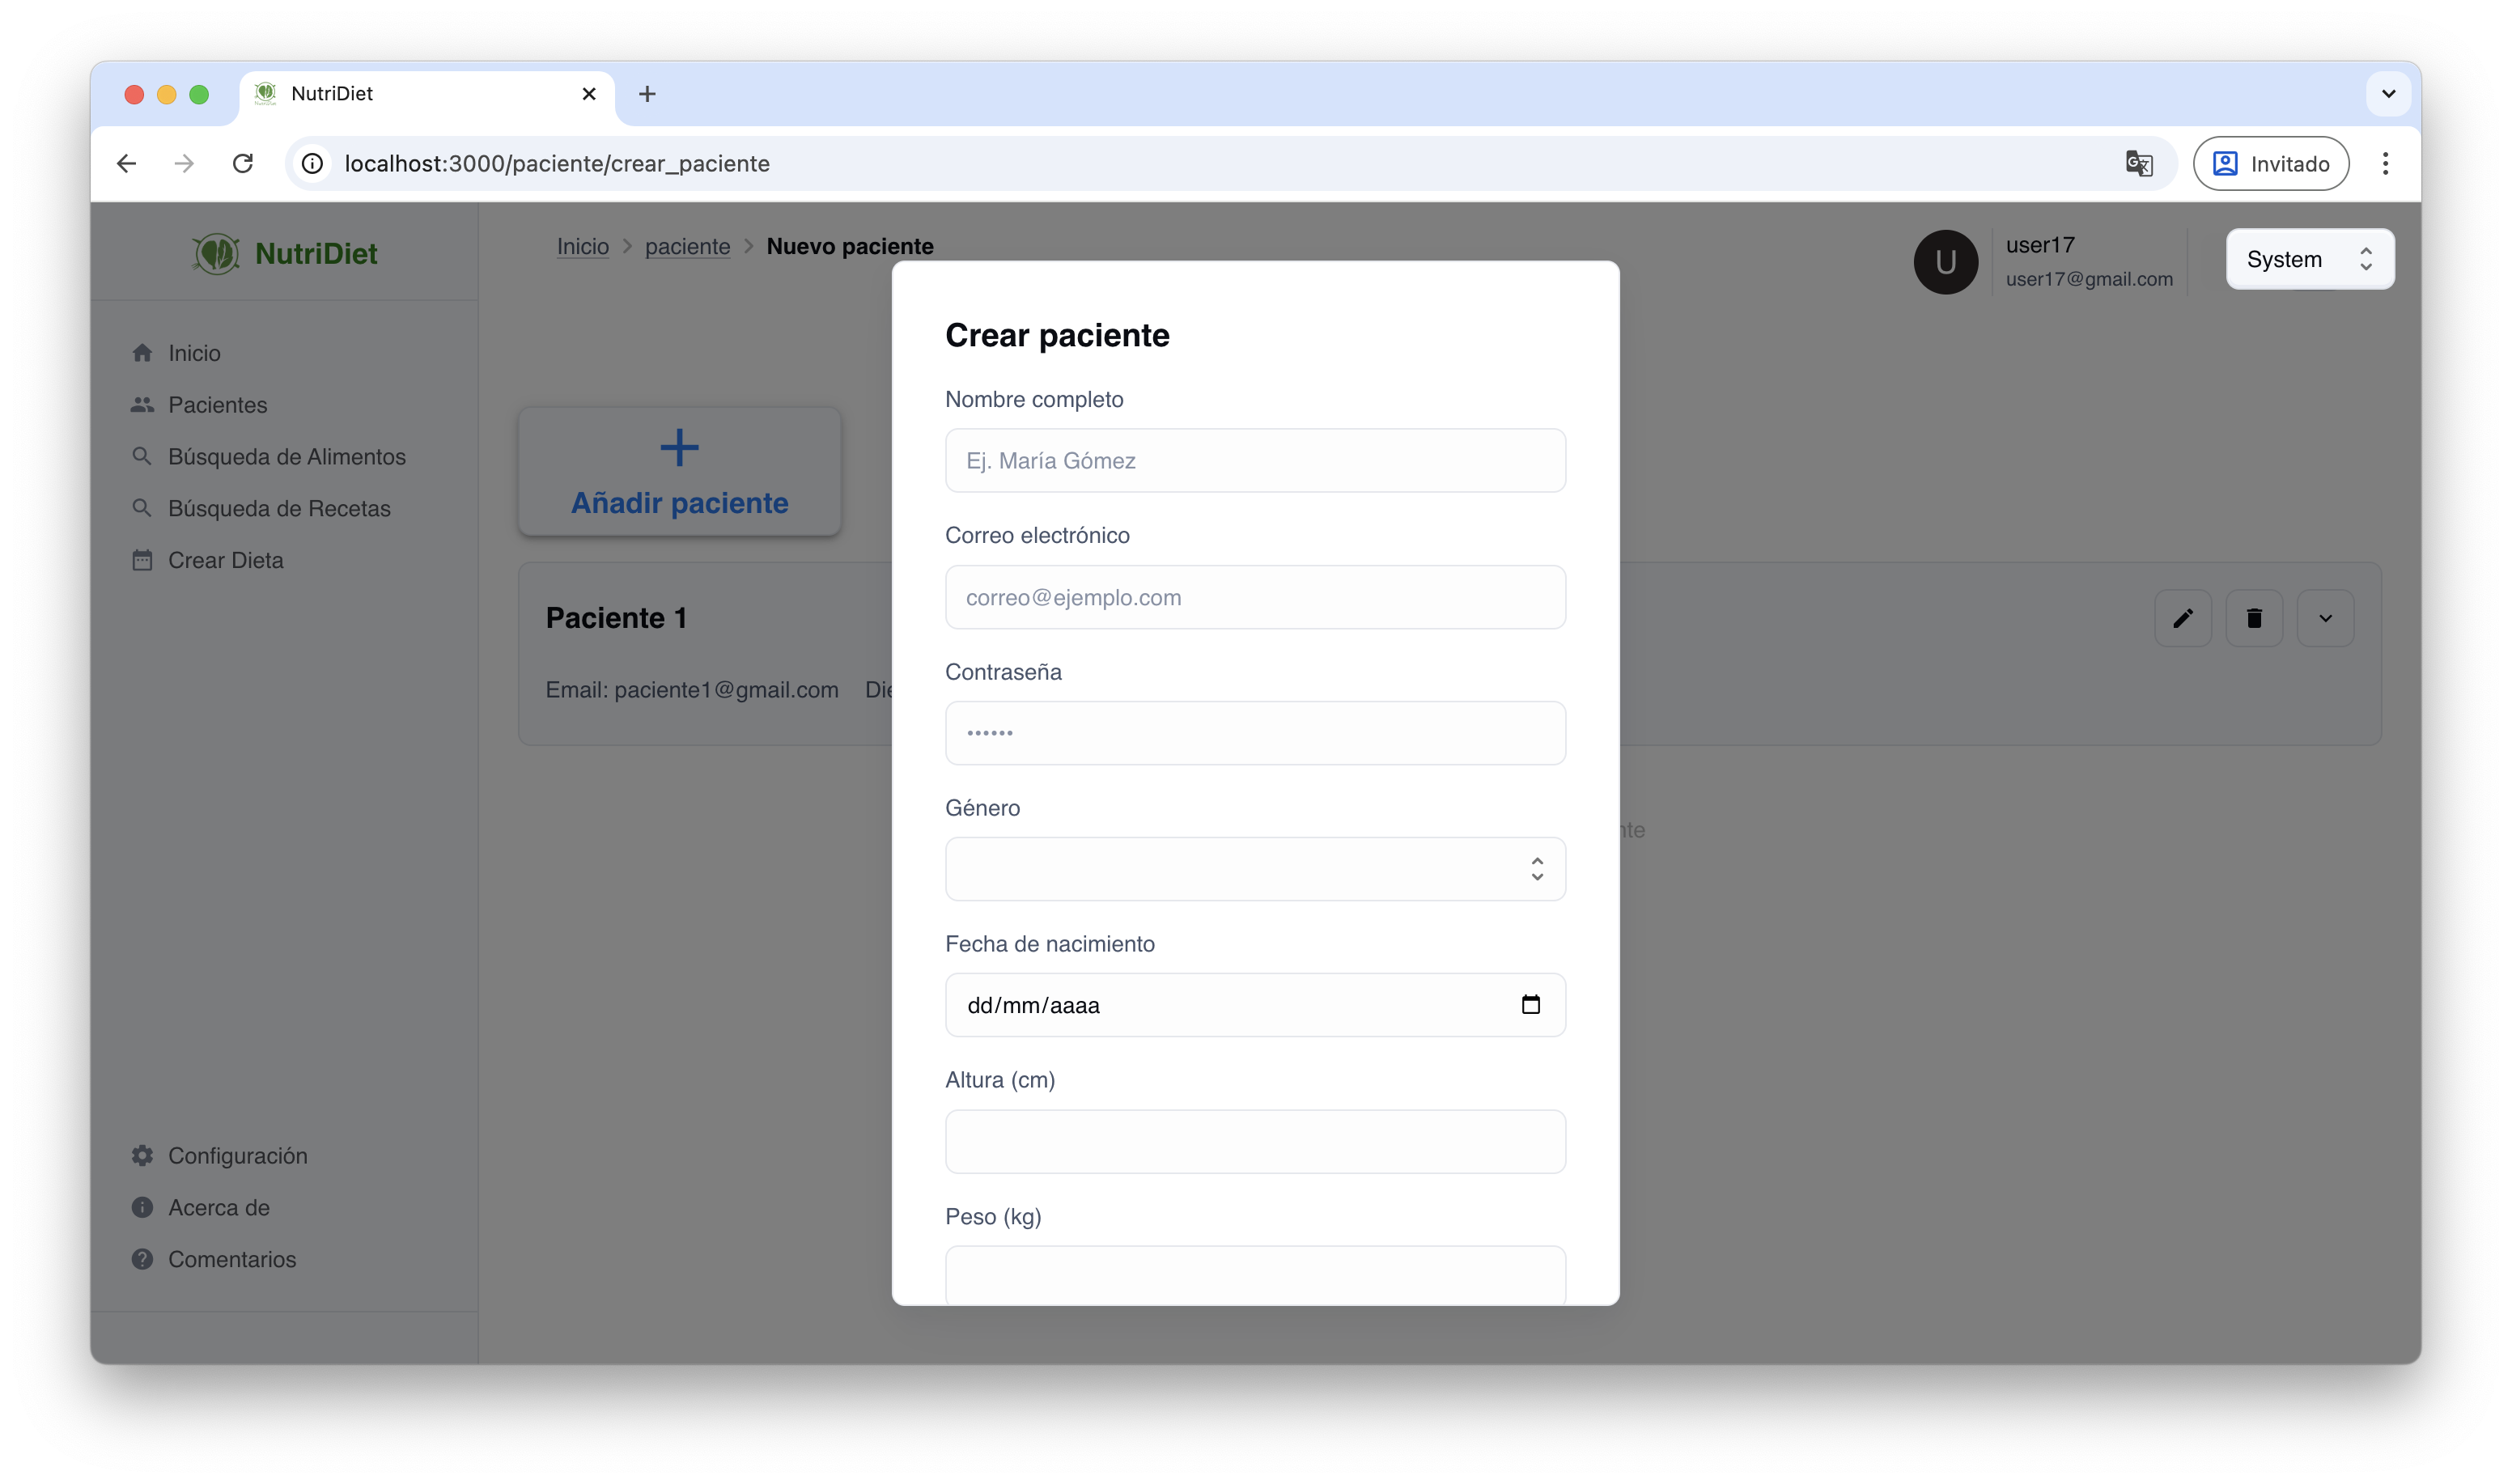
\includegraphics[width=1\linewidth]{Plantilla_TFG_latex//imagenes/Paciente_crearP.png}
    \caption{Formulario de creación de un nuevo paciente}
    \label{fig:Paciente_crearP}
\end{figure}

\subsection{Visualización detallada de dietas}
Mediante el botón ``Ver dieta'', el usuario puede acceder al detalle completo de una dieta asignada a un paciente. Esta vista muestra el nombre de la dieta, el periodo de validez, el nombre del paciente y el nutricionista responsable (Figura~\ref{fig:detalle_dieta_visual}). A continuación, se presenta una tabla diaria con las ingestas planificadas, donde se agrupan las recetas por tipo (desayuno, almuerzo, cena, etc.) y subtipo (primer plato, bebida, postre, etc.). Para cada receta incluye un botón para acceder a su ficha completa. 
\begin{figure}
    \centering
    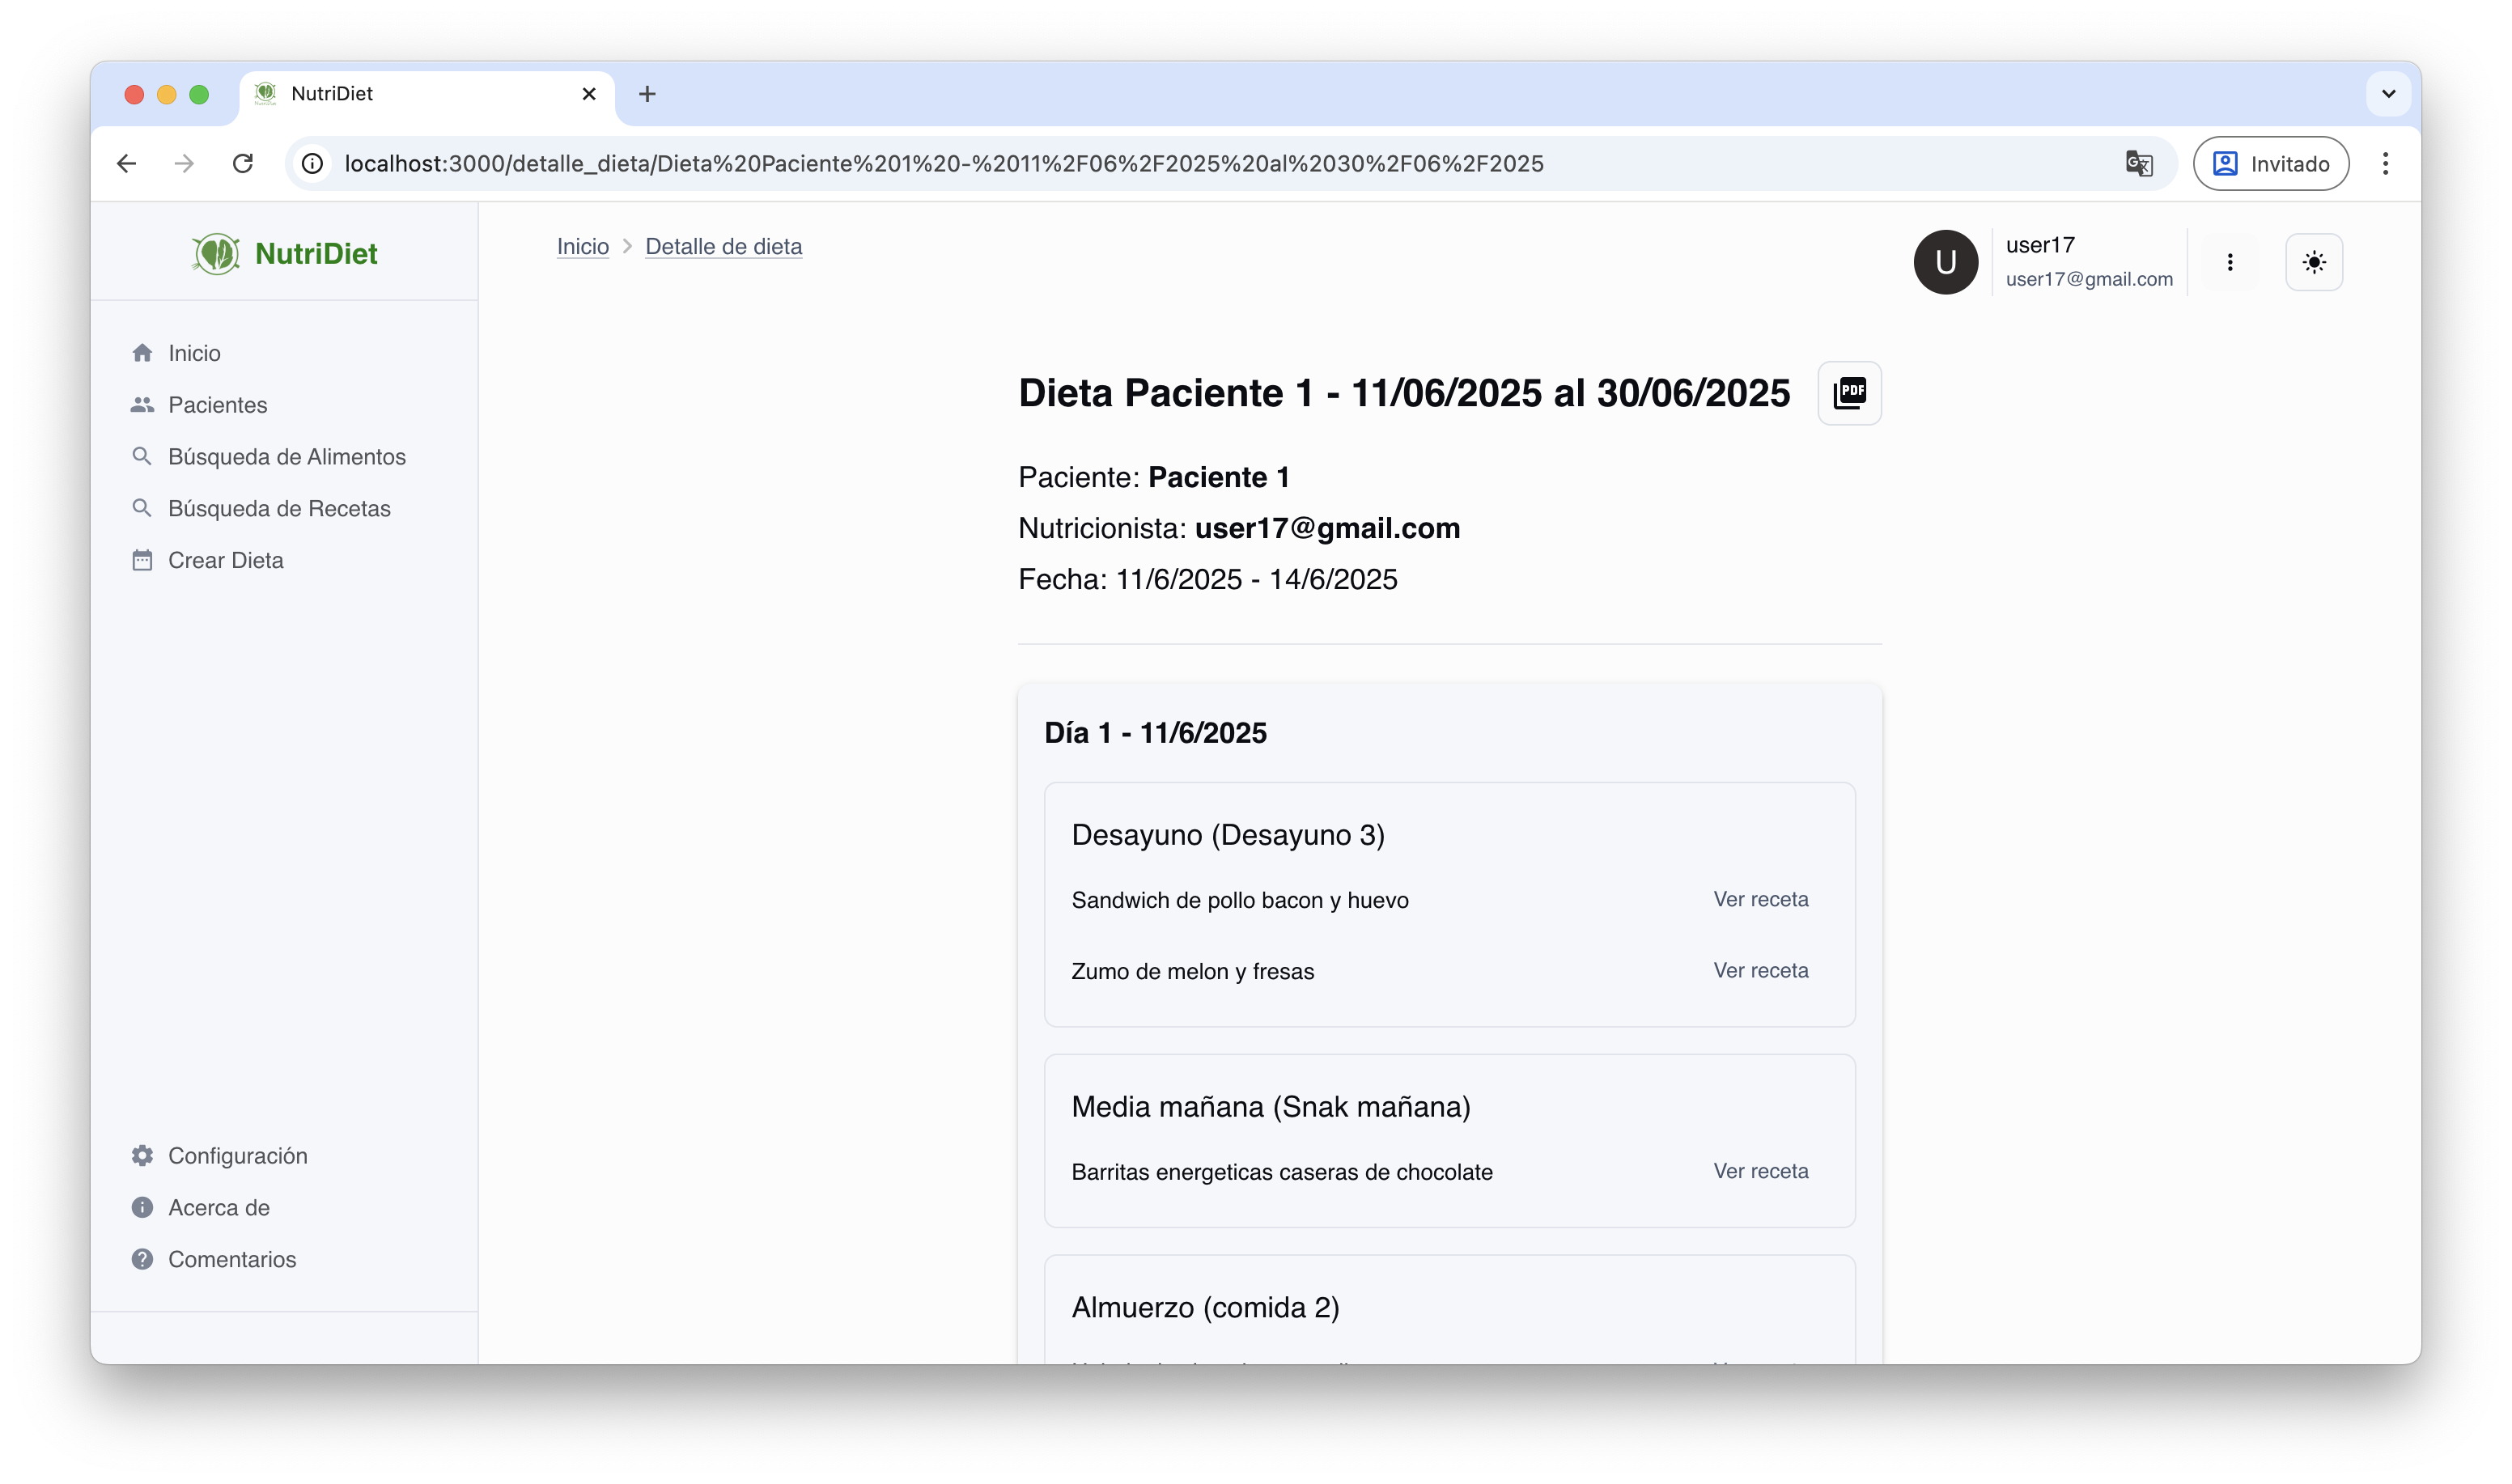
\includegraphics[width=1\linewidth]{Plantilla_TFG_latex/imagenes/PagPaciente_detalleDieta.png}
    \caption{Vista detallada de una dieta asignada a un paciente}
    \label{fig:detalle_dieta_visual}
\end{figure}

\begin{figure}
    \centering
    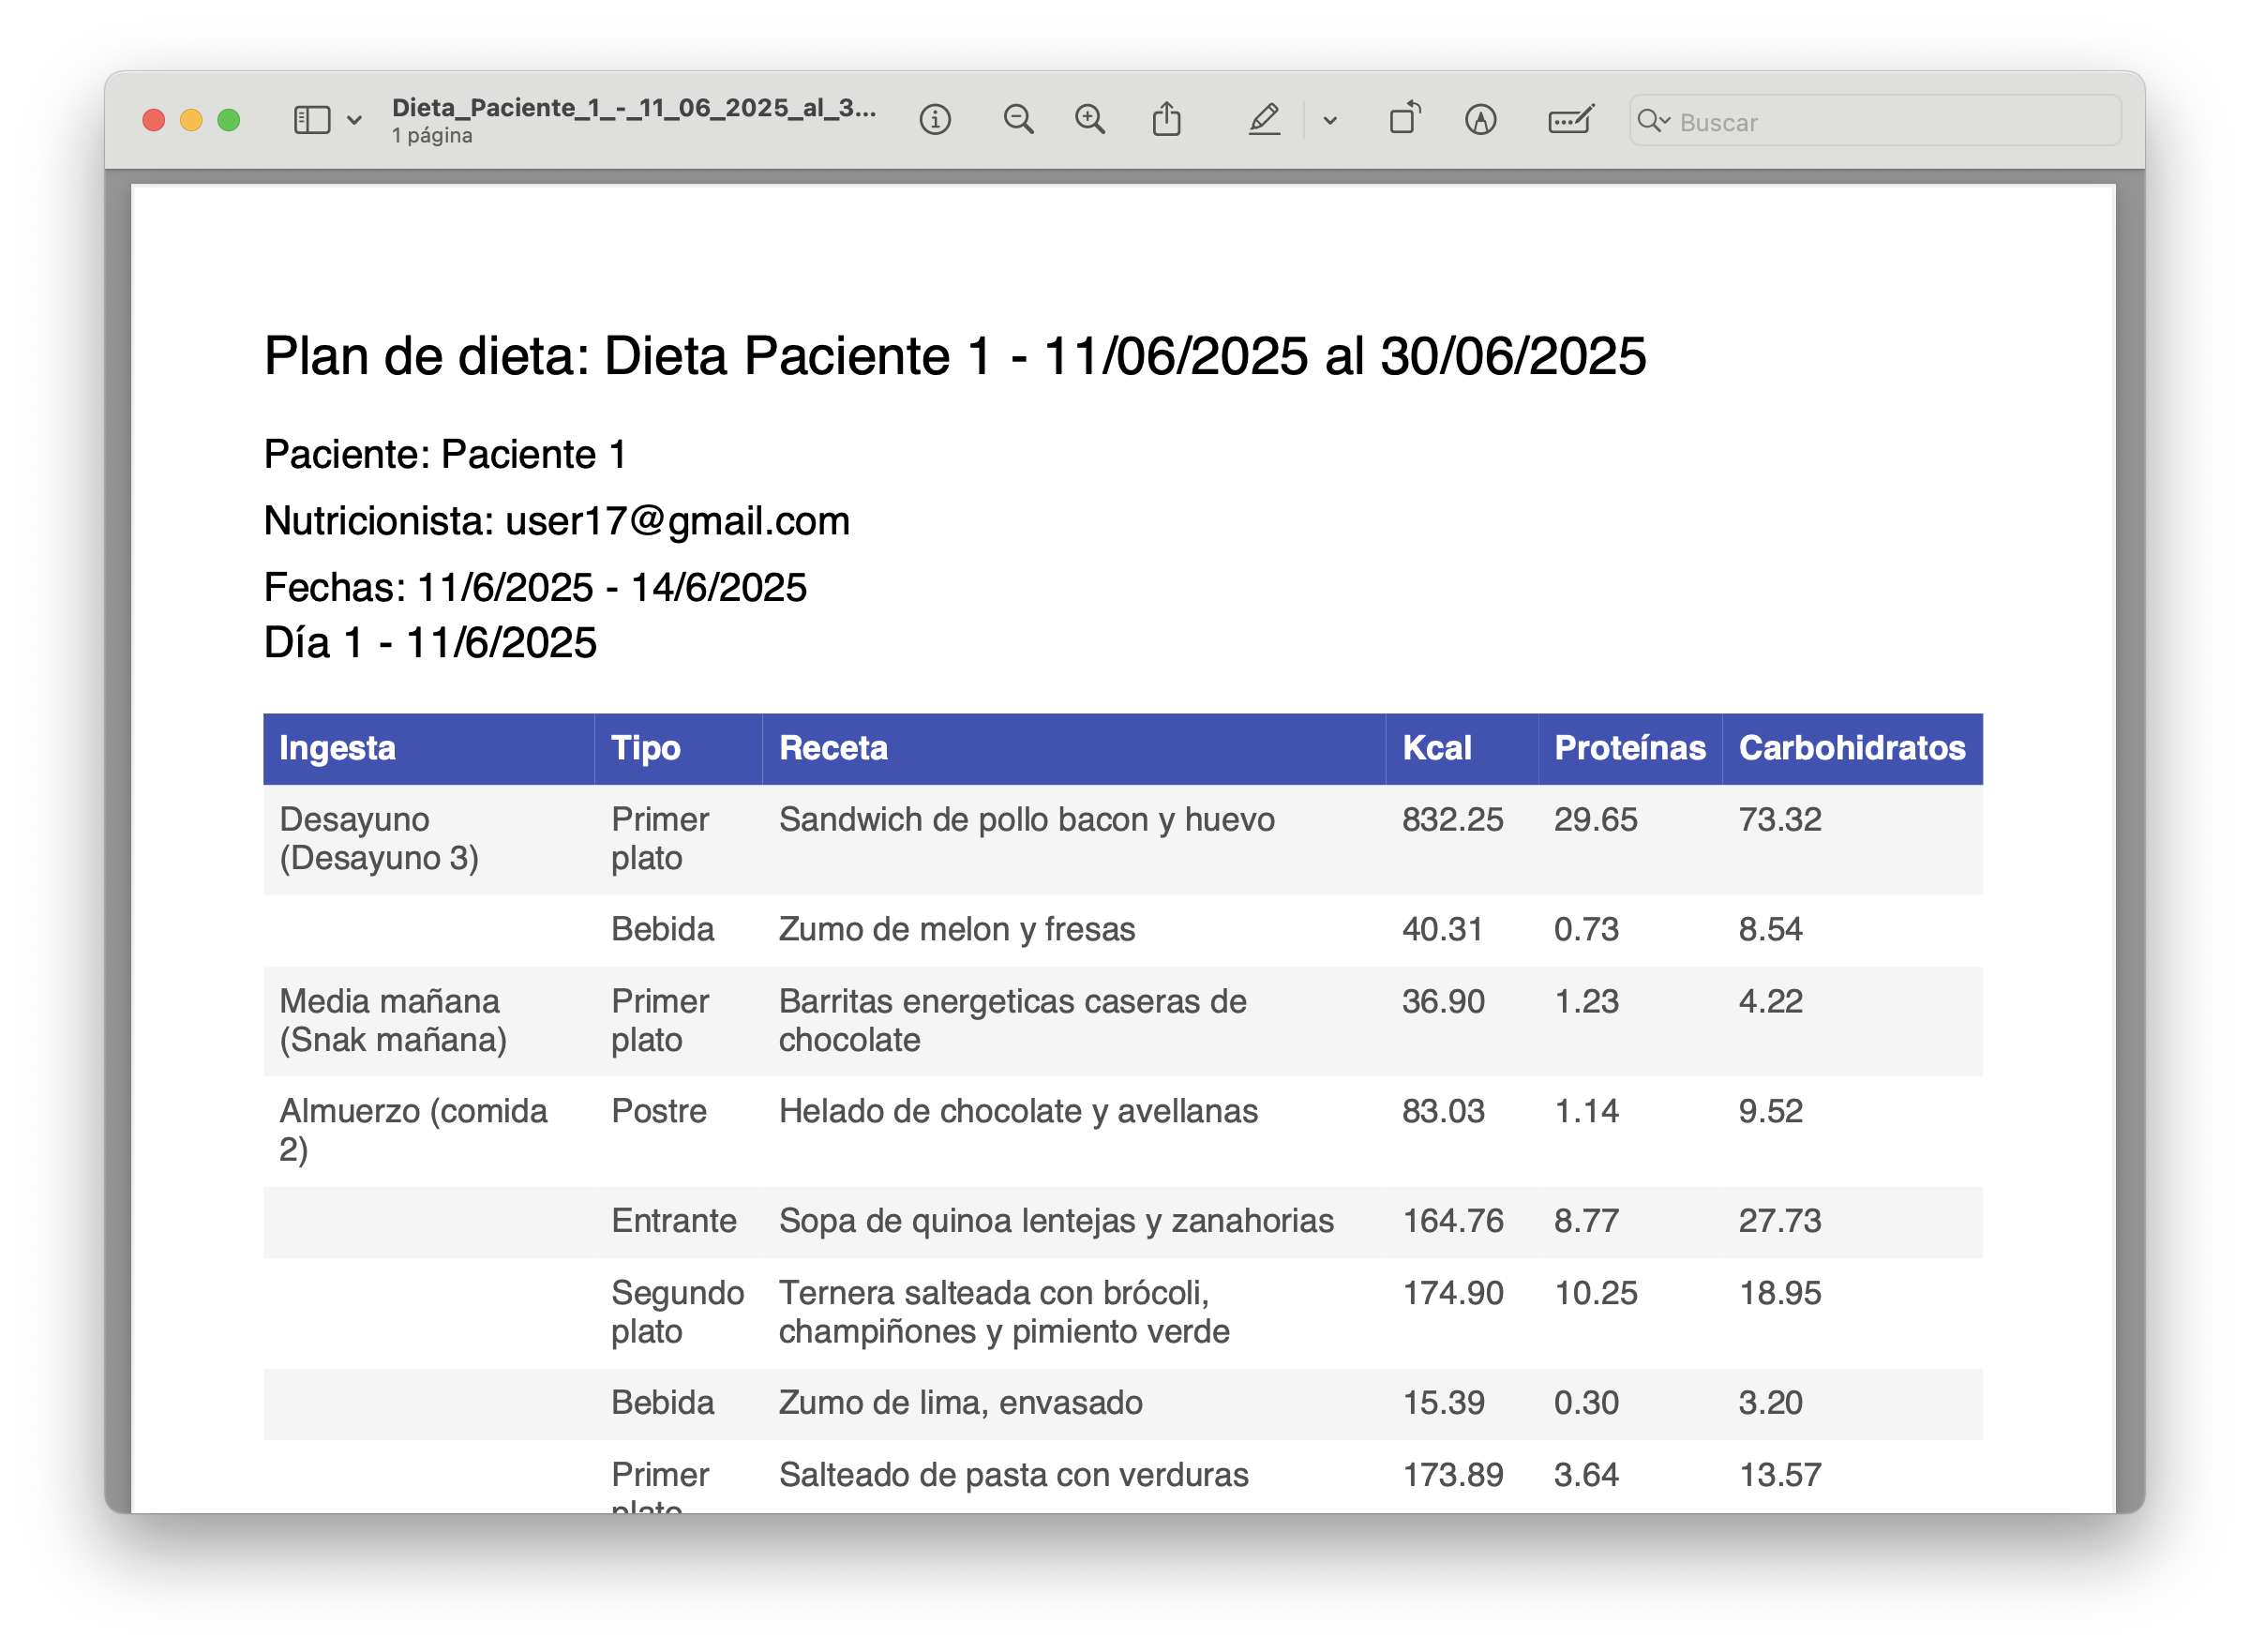
\includegraphics[width=1\linewidth]{Plantilla_TFG_latex/imagenes/PagPaciente_detalleD_PDF.png}
    \caption{Vista del documento PDF generado con el detalle nutricional diario de la dieta}
    \label{fig:detalle_dieta_pdf}
\end{figure}


La interfaz también permite descargar la dieta en formato PDF, incluyendo toda la información estructurada por días: ingestas, recetas, tipo de plato y valores nutricionales detallados (Figura~\ref{fig:detalle_dieta_pdf}). Además, se muestra un resumen diario con el total de kilocalorías, proteínas y carbohidratos, lo que facilita el análisis nutricional del plan. Esta funcionalidad es especialmente importante para el trabajo del nutricionista, ya que permite disponer de una versión imprimible y ordenada del plan dietético, útil tanto para la consulta como para el seguimiento del paciente. De hecho, se trata de un requerimiento expresamente planteado por el profesorado del área de nutrición, quienes lo consideran esencial en el uso docente.


\section{Consultas de alimentos}
El sistema incluye una sección dedicada a la visualización y consulta de alimentos (Figura~\ref{fig:Alimento_ini}), con el objetivo de proporcionar información nutricional precisa y estandarizada. 

\begin{itemize}
    \item Listado de alimentos: Muestra todos los alimentos disponibles en el sistema divididos por categoría.
    
    \item Búsqueda y filtrado: Permite buscar por nombre y filtrar los alimentos por categoría, letra inicial o composición nutricional esencial.

    \item Detalle del alimento: Al seleccionar un alimento se accede a su información nutricional completa. Cada alimento incluye medidas estándar y caseras para facilitar su uso práctico.
\end{itemize}

\begin{figure}[H]
    \centering
    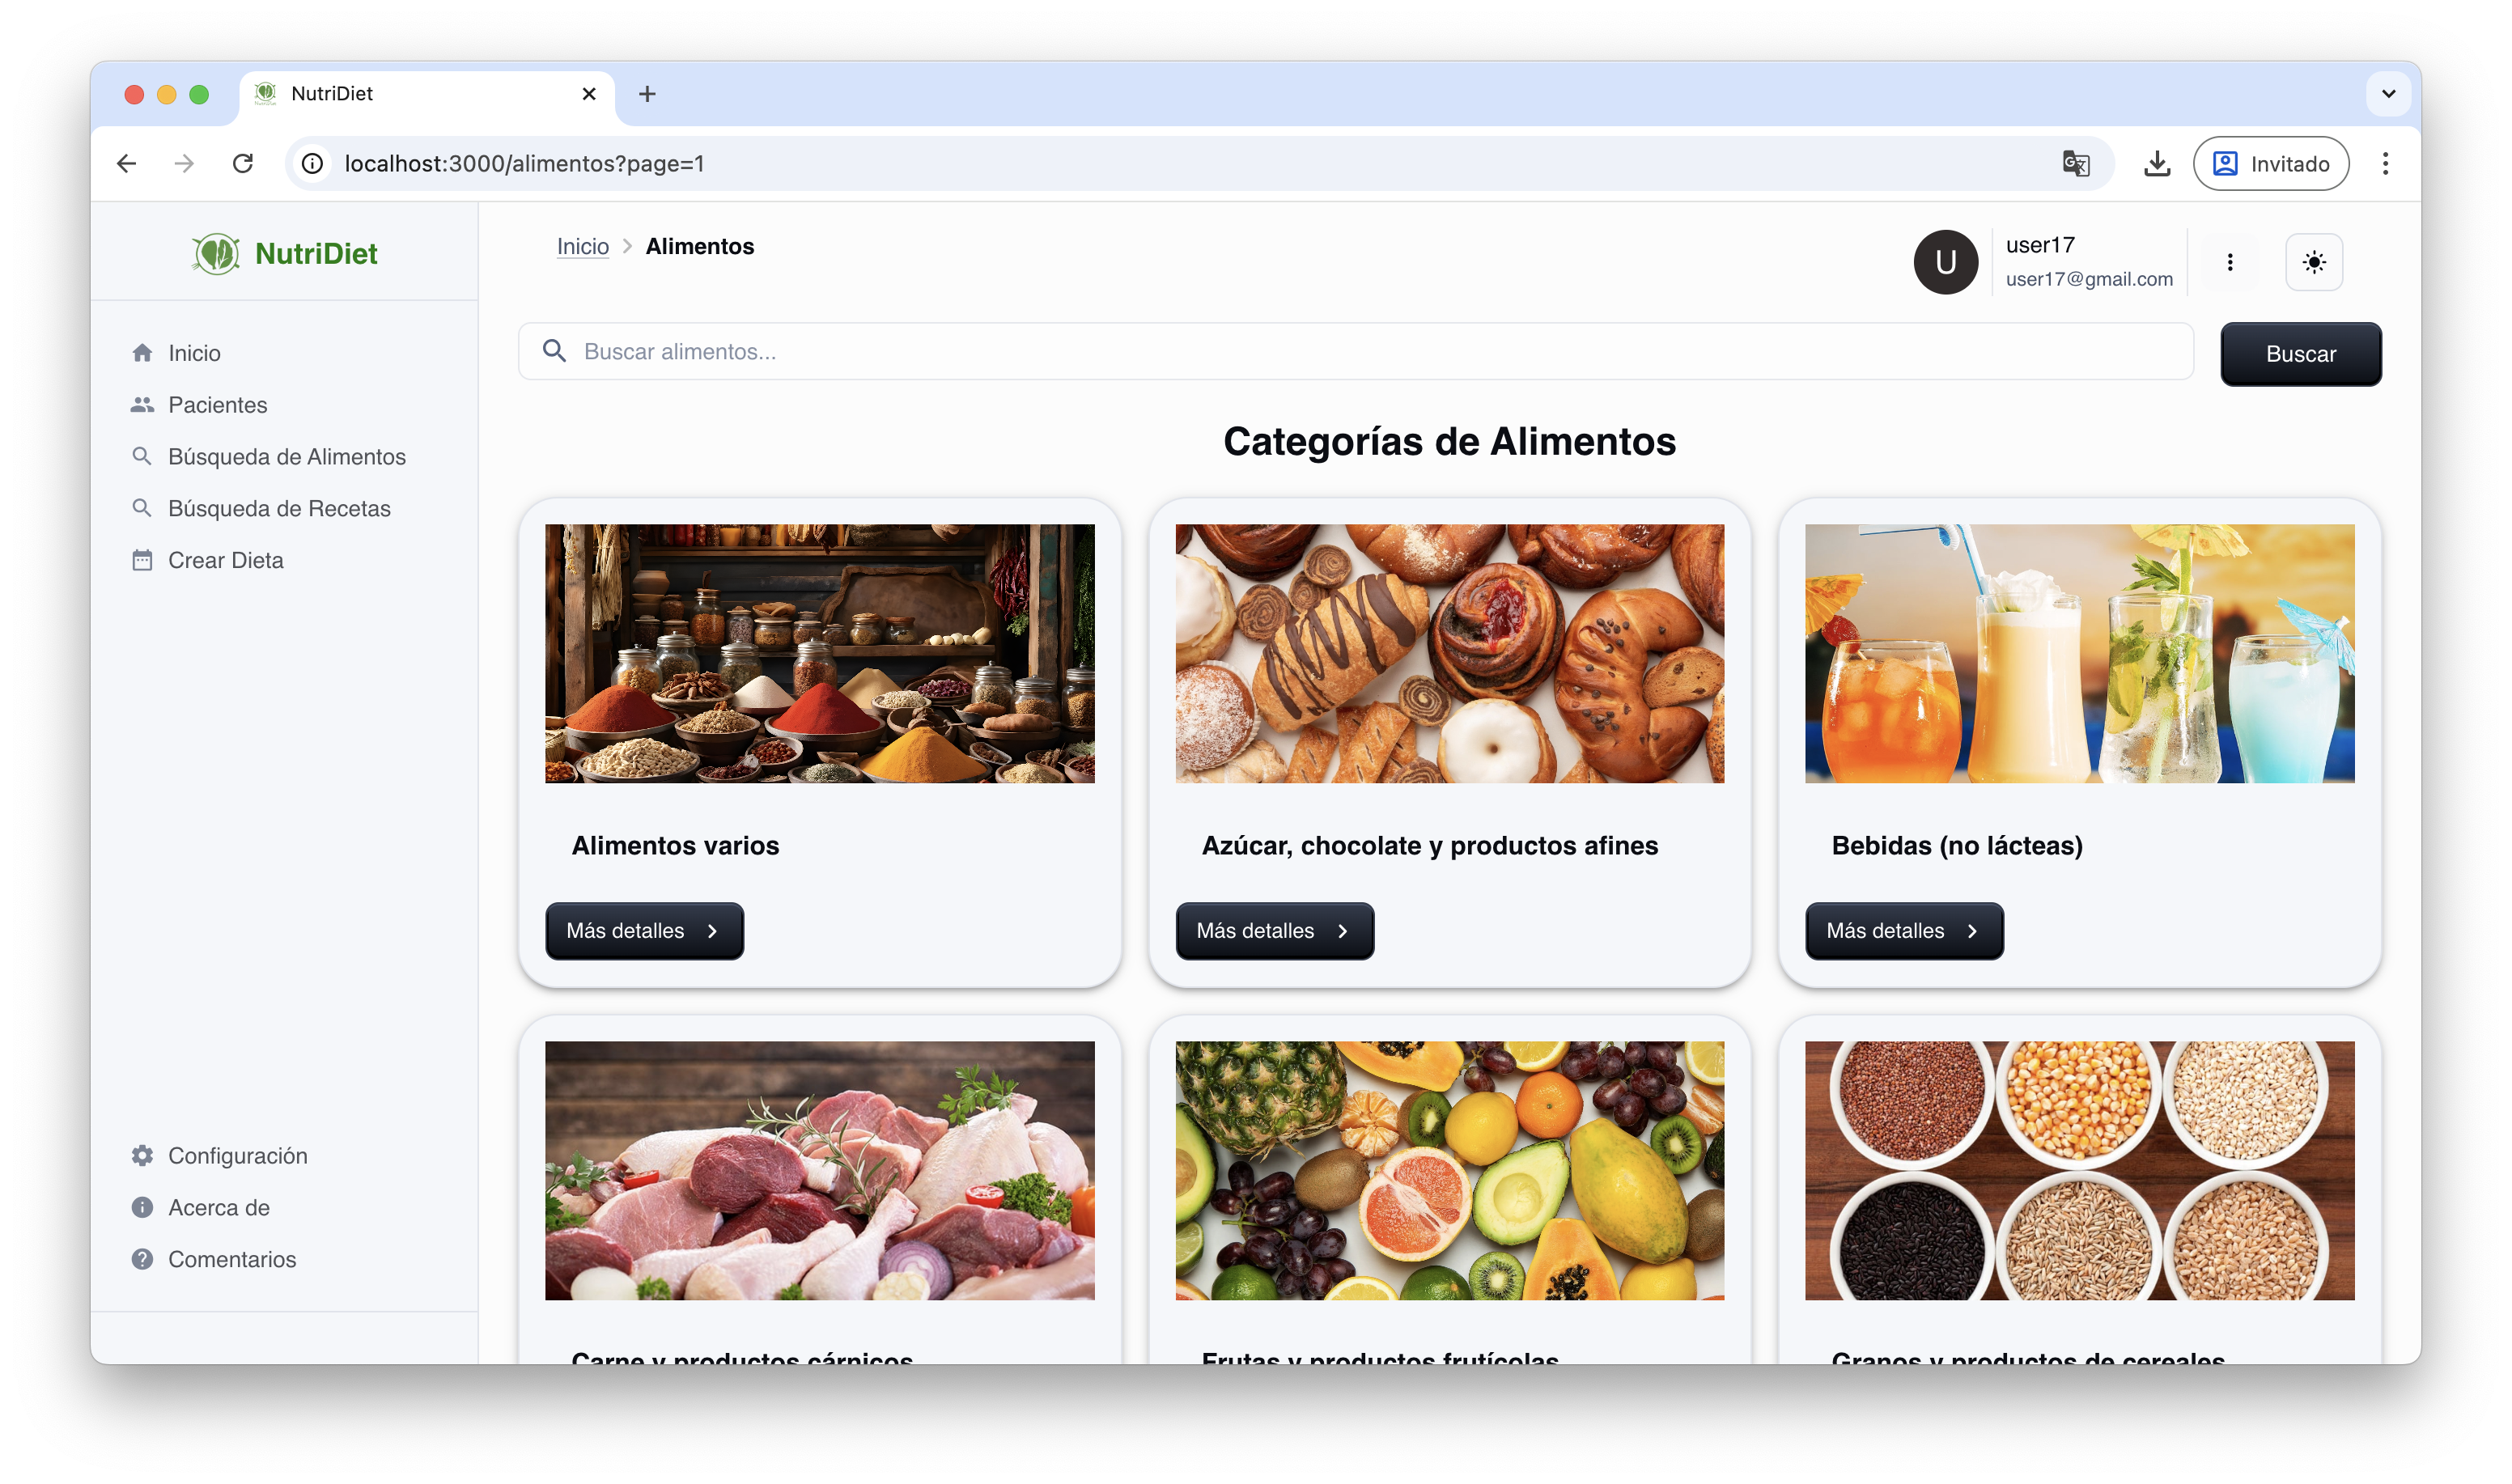
\includegraphics[width=1\linewidth]{Plantilla_TFG_latex//imagenes/Alimento_ini.png}
    \caption{Vista general del módulo de alimentos}
    \label{fig:Alimento_ini}
\end{figure}

\subsection{Búsqueda y filtrado}
El sistema proporciona una herramienta de búsqueda y filtrado avanzada para facilitar la localización de alimentos en la base de datos (Figura~\ref{fig:Alimento_Categoria}).

La barra de búsqueda permite introducir el nombre (completo o parcial) del alimento, mostrando como máximo los primeros 20 resultados coincidentes. A medida que el usuario escribe, los resultados se actualizan dinámicamente en tiempo real. 

Además de la búsqueda por texto, el sistema incluye múltiples opciones de filtrado combinables entre sí:

\begin{itemize}
    \item Por categoría: permite mostrar solo alimentos pertenecientes a un grupo específico (por ejemplo: frutas, carnes, cereales, etc.).
    
    \item Por letra inicial: útil para localizar alimentos cuando solo se conoce la primera letra del nombre (A–Z).
    
    \item Por nivel de nutrientes: el usuario puede filtrar alimentos según su contenido en sodio, azúcar o grasa, seleccionando entre tres rangos: bajo, medio o alto. Permite identificar rápidamente alimentos más saludables o adaptados a dietas específicas (como hiposódicas o bajas en azúcares).
\end{itemize}

\begin{figure}[H]
    \centering
    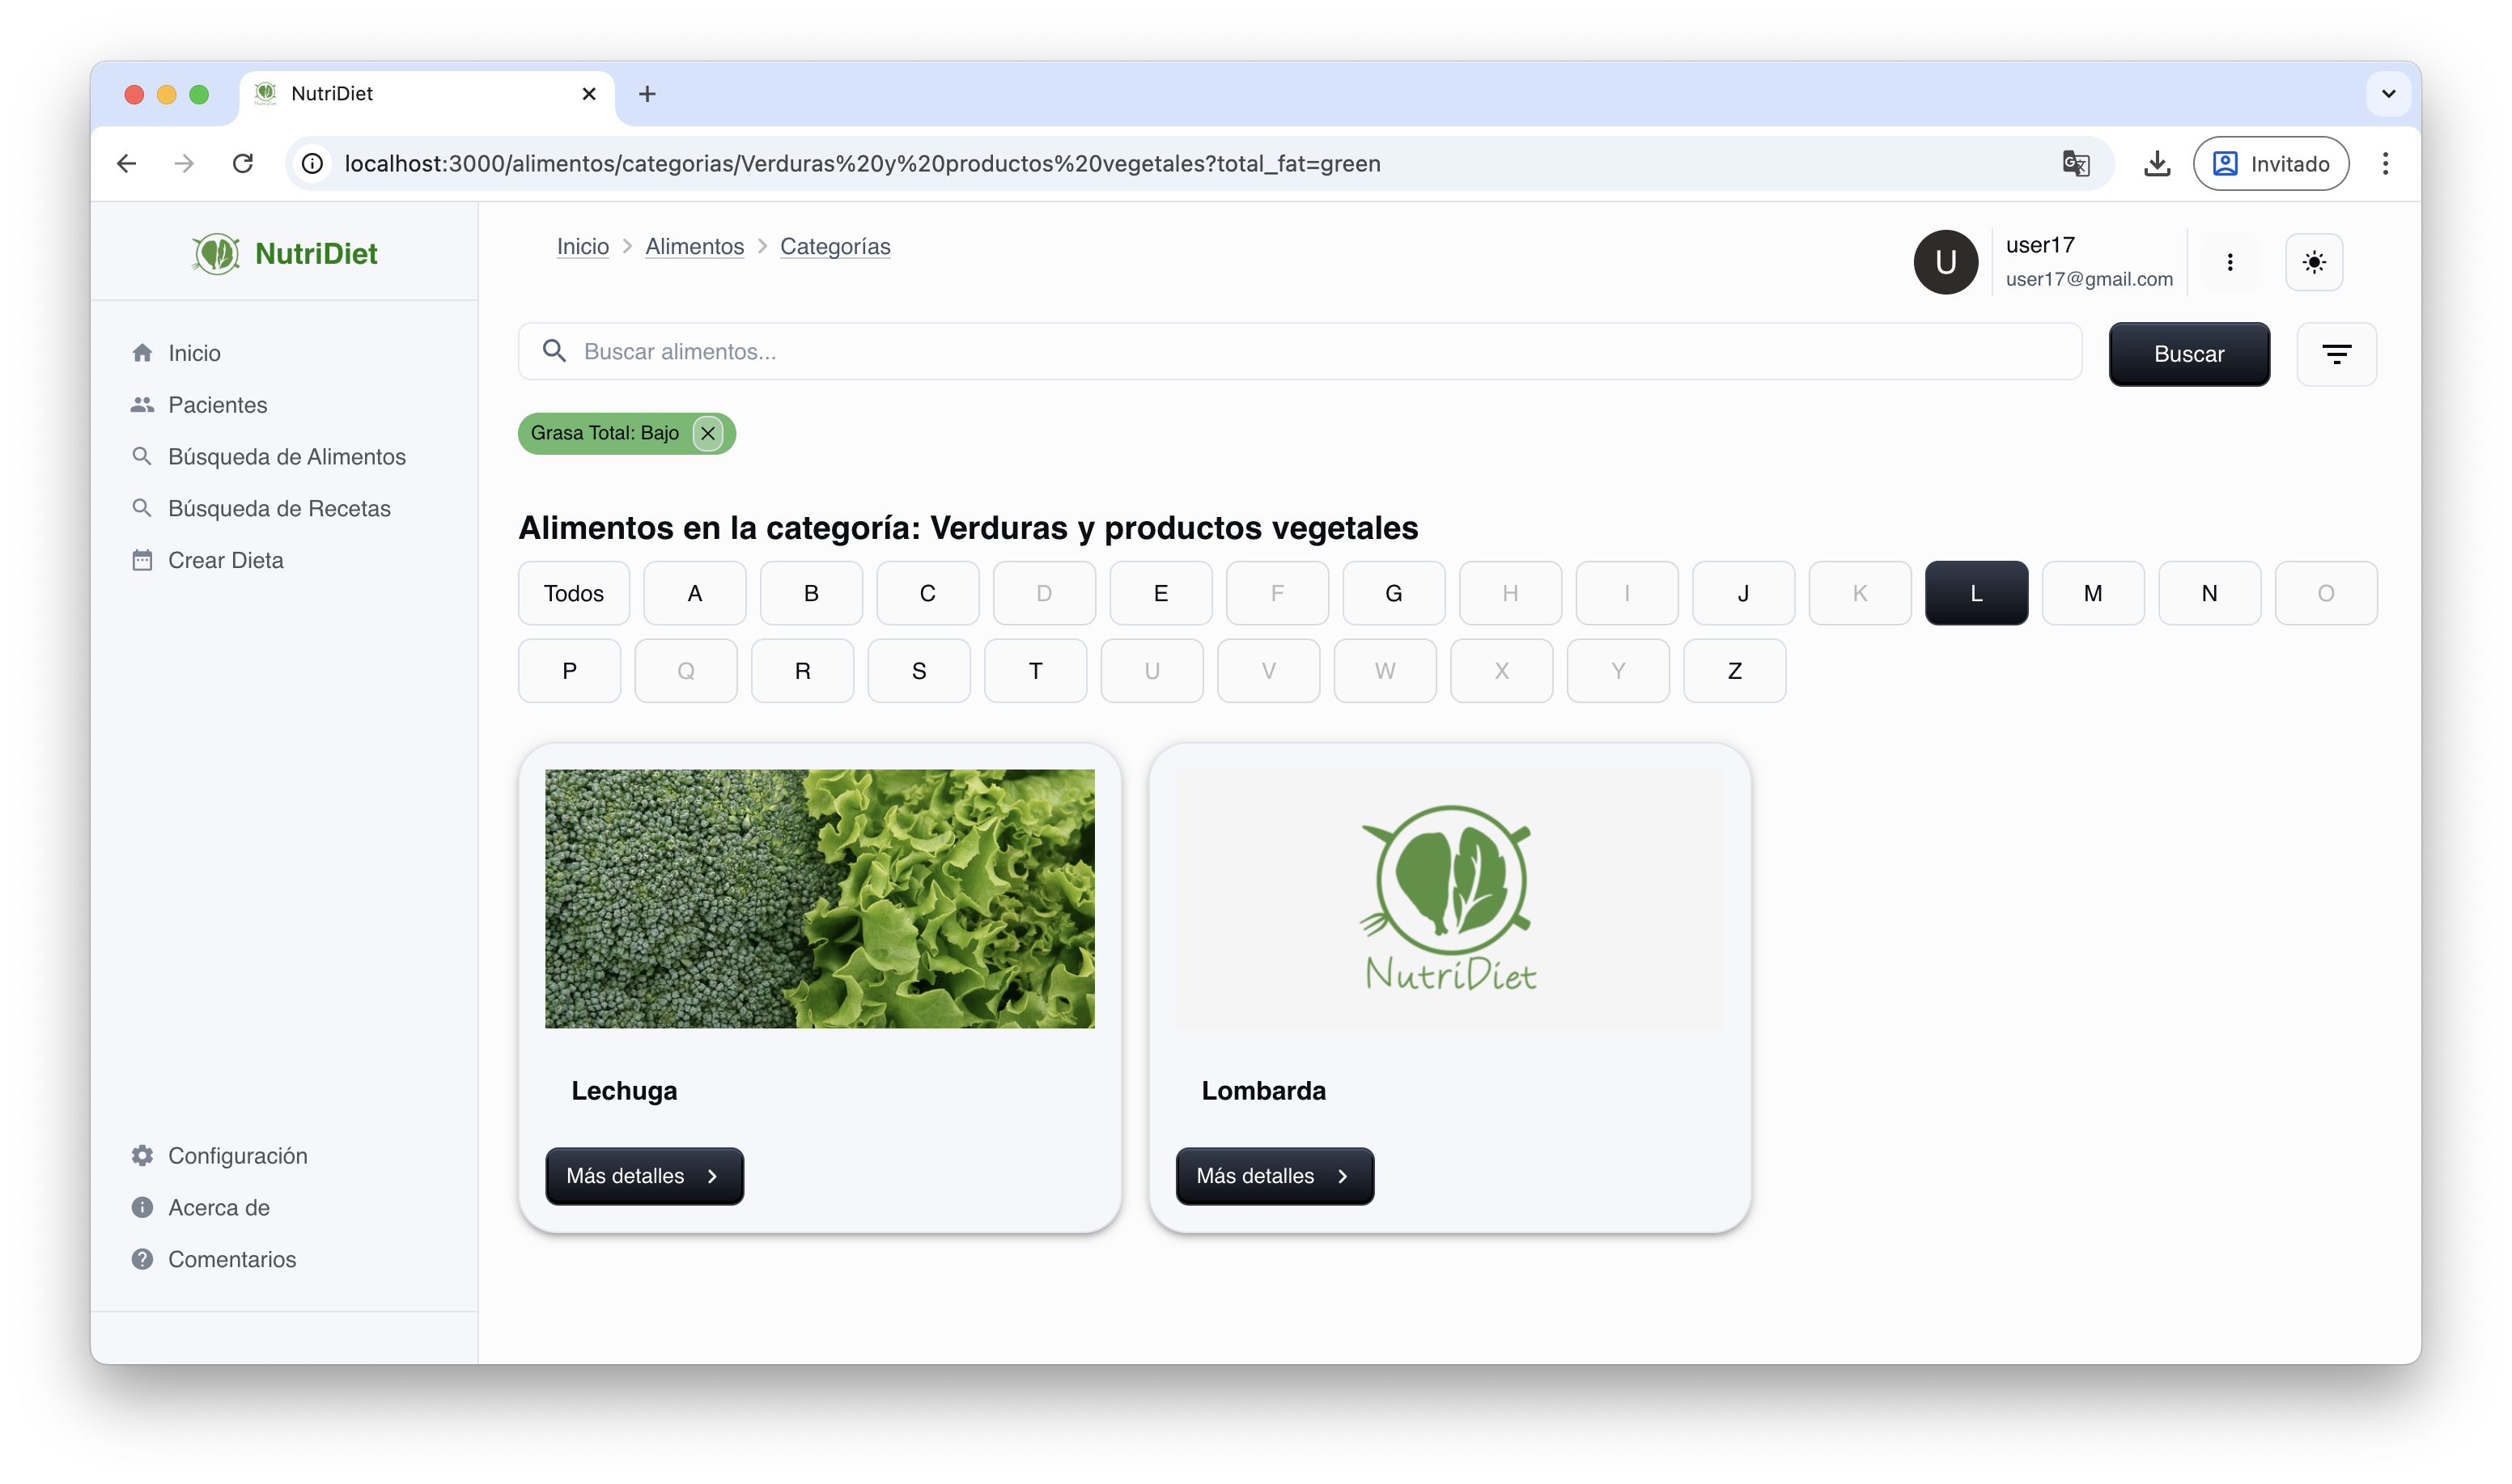
\includegraphics[width=1\linewidth]{Plantilla_TFG_latex/imagenes/Alimento_Categoria.png}
    \caption{Interfaz de búsqueda y filtrado de alimentos por nombre, categoría, letra inicial y contenido nutricional}
    \label{fig:Alimento_Categoria}
\end{figure}

\subsection{Detalle del alimento}
Esta vista muestra la información nutricional completa y organizada, acompañada de una imagen representativa, su categoría, el porcentaje comestible y el etiquetado nutricional según el sistema de semáforos de la OMS (sal, azúcar, grasa) (Figura~\ref{fig:detalle_alimento}).

En la parte principal se encuentra una tabla que presenta los valores nutricionales por 100 gramos, por porción comestible y por diferentes medidas prácticas (porciones estándar, unidades y medidas caseras como “1 cucharada” o “1 taza”), lo cual permite adaptar fácilmente el uso del alimento en recetas o dietas.

\begin{figure}[H]
    \centering
    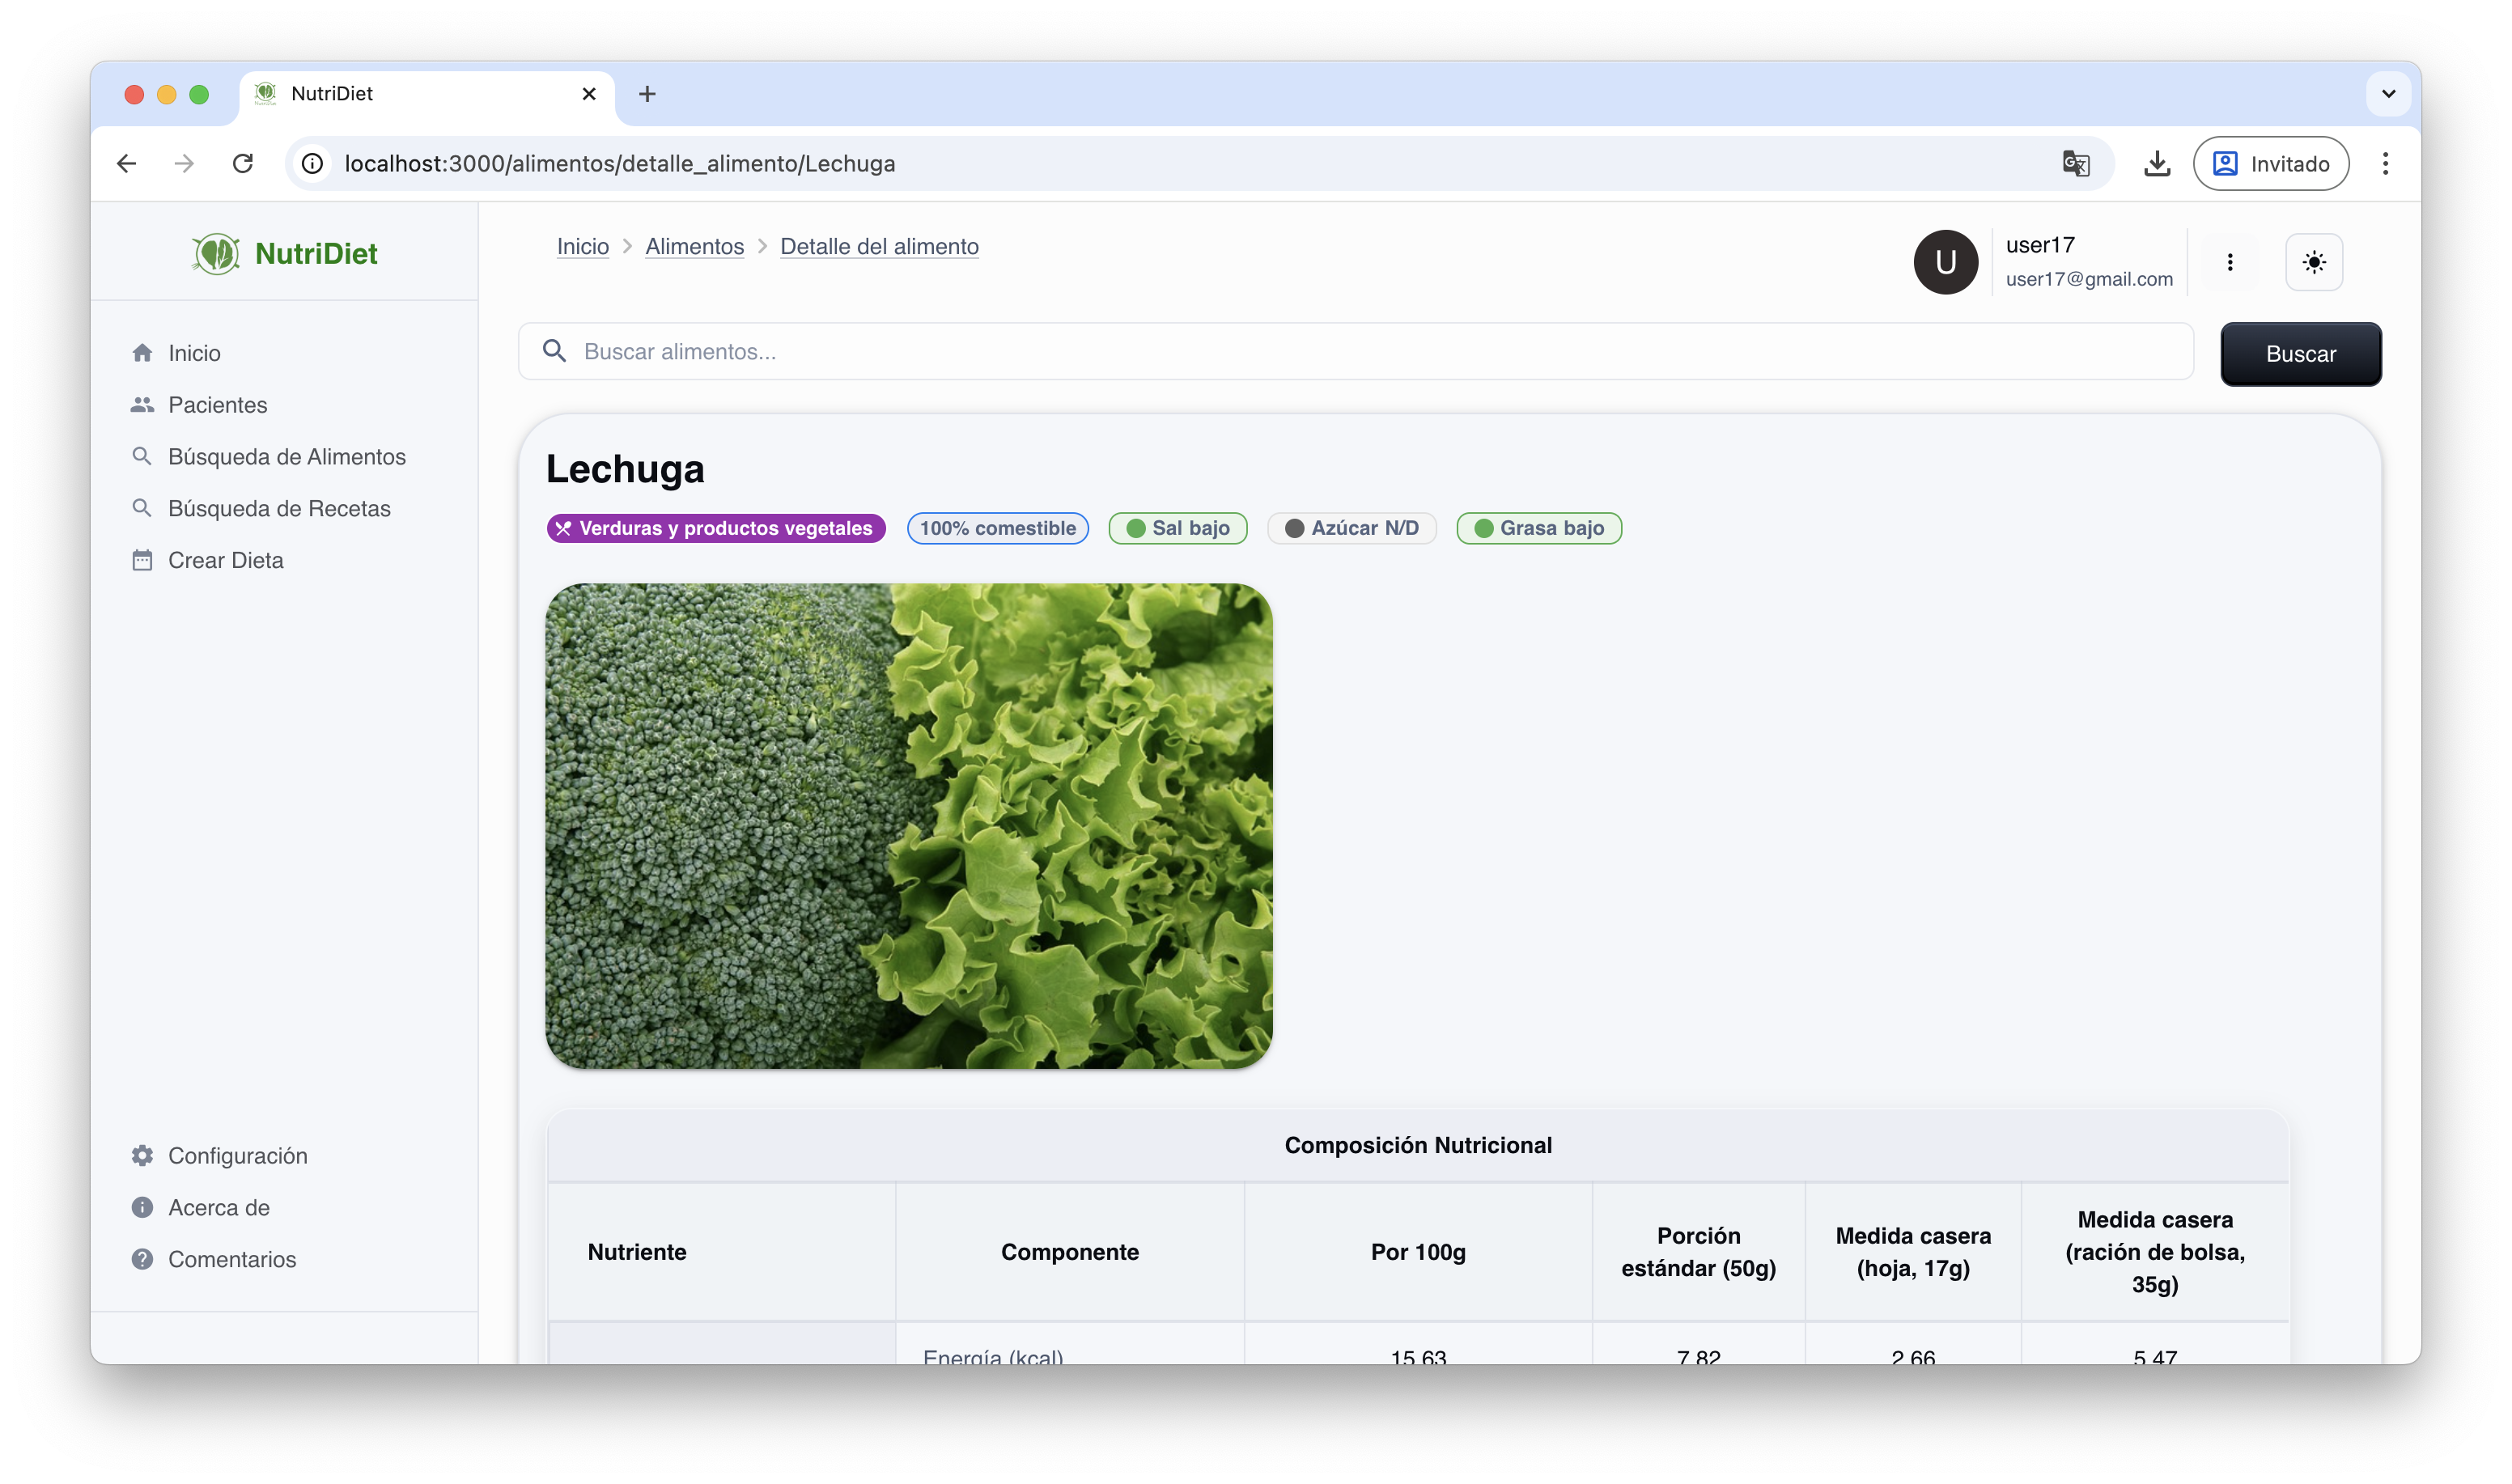
\includegraphics[width=1\linewidth]{Plantilla_TFG_latex/imagenes/PagAlimento_Detalle.png}
    \caption{Vista detallada de un alimento con tabla nutricional y porciones disponibles}
    \label{fig:detalle_alimento}
\end{figure}

\section{Consultas de recetas}
El sistema incluye un módulo específico para la búsqueda y visualización de recetas (Figura~\ref{fig:consultas_recetas}). Desde esta sección, el usuario puede explorar todas las recetas registradas, ya sea mediante navegación libre o utilizando herramientas de búsqueda y filtrado por categoría.

\begin{itemize}
    \item Listado de recetas: Muestra todas las recetas disponibles en formato de tarjetas, organizadas por categoría.

    \item Búsqueda y filtrado: Permite buscar recetas por nombre y aplicar filtros por categoría, letra inicial o por valores nutricionales (kcal, proteínas, carbohidratos).

    \item Detalle de receta: Al seleccionar una receta, se muestra su composición nutricional completa, los ingredientes, número de raciones, los pasos de preparación y un pequeño comentario nutricional.
\end{itemize}

\begin{figure}[t]
    \centering
    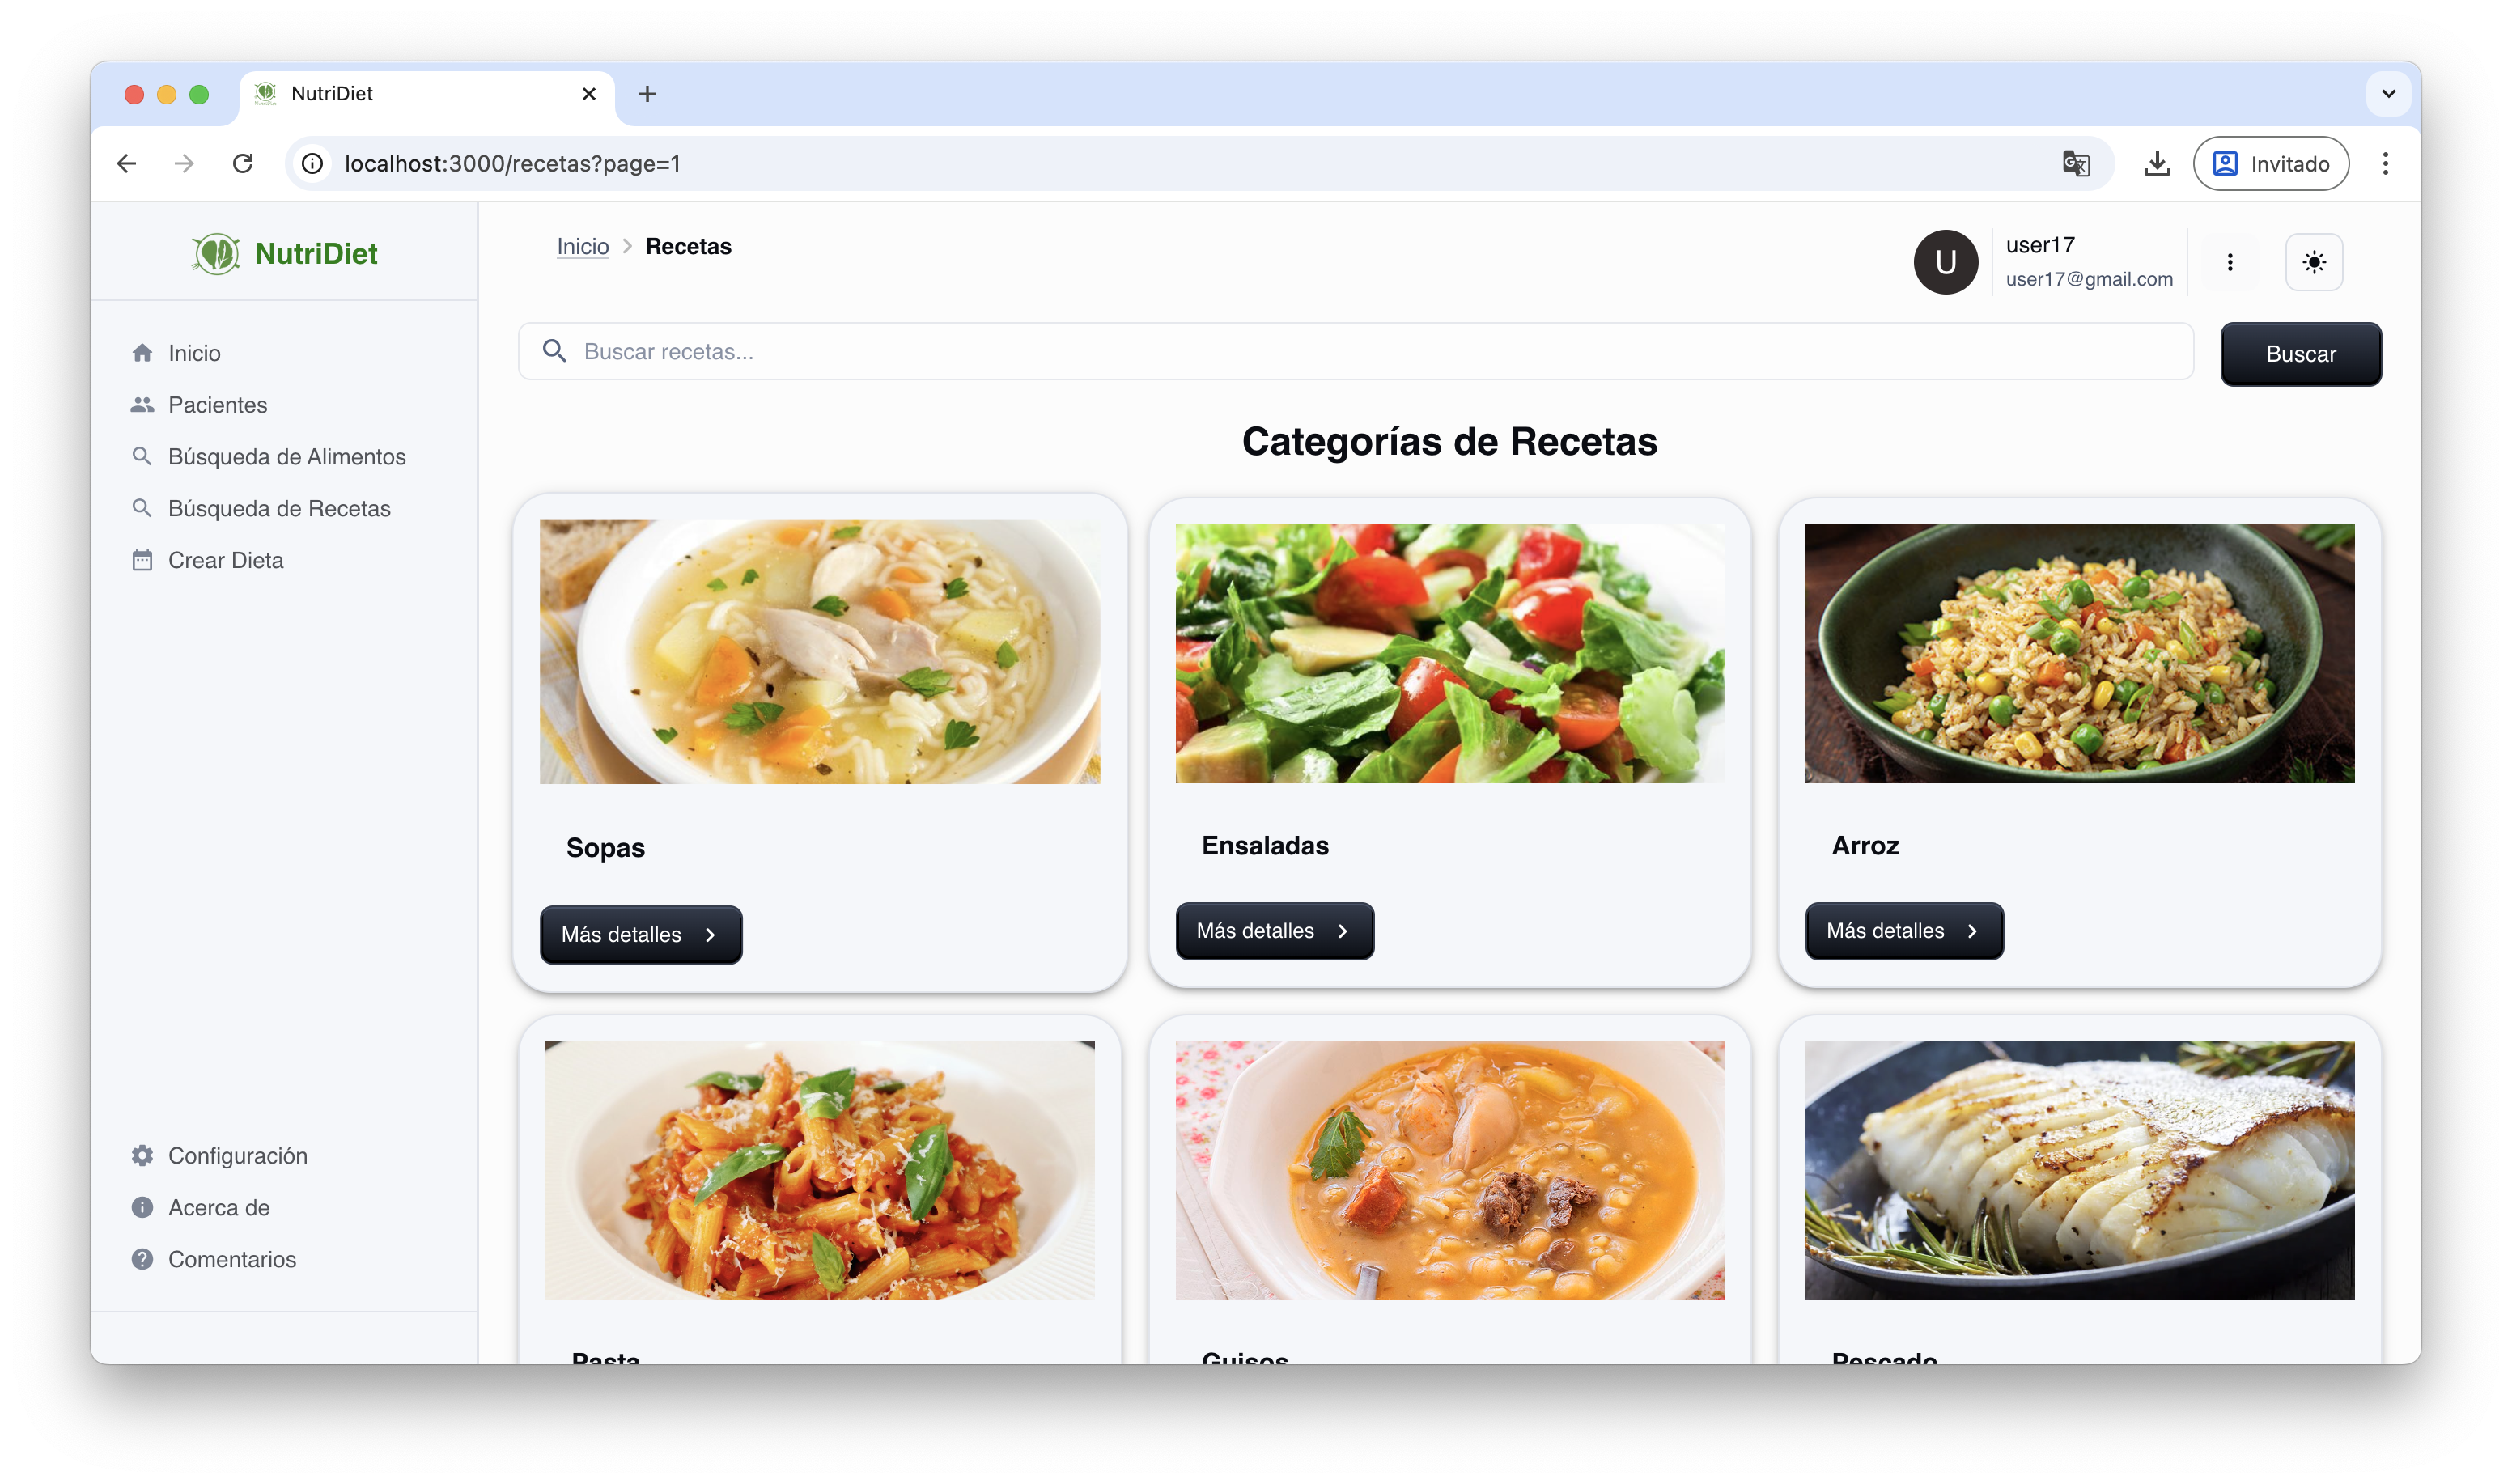
\includegraphics[width=1\linewidth]{Plantilla_TFG_latex/imagenes/Recetas_ini.png}
    \caption{Vista general del módulo de recetas con tarjetas filtrables por categoría}
    \label{fig:consultas_recetas}
\end{figure}

\subsection{Búsqueda y filtrado}
El sistema ofrece una interfaz avanzada para la búsqueda y filtrado de recetas dentro de una categoría específica. (Figura~\ref{fig:Recetas_categoria})  Esta funcionalidad permite al usuario localizar fácilmente recetas que se ajusten tanto a criterios textuales como a parámetros nutricionales específicos.

La barra de búsqueda acepta el nombre completo o parcial de una receta. A medida que se escribe, se despliega una lista de sugerencias dinámicas que permite seleccionar directamente una receta y acceder a su detalle. Este sistema de autocompletado mejora la rapidez y precisión de la búsqueda.

Además de la búsqueda textual, se incluyen varias opciones de filtrado que pueden combinarse:

\begin{itemize}
    \item Por letra inicial: muestra únicamente las recetas cuyo nombre comienza por la letra seleccionada (de la A a la Z), facilitando una exploración rápida cuando se desconoce el nombre exacto.

    \item Por contenido nutricional: el usuario puede activar filtros avanzados que permiten establecer rangos personalizados para calorías, proteínas y carbohidratos. Esta funcionalidad resulta útil para identificar recetas adaptadas a necesidades nutricionales concretas (por ejemplo, dietas hipocalóricas o altas en proteínas). Los rangos máximos se ajustan automáticamente según las recetas disponibles en la categoría.

    \item Paginación y visualización: las recetas que cumplen los criterios de búsqueda y filtrado se muestran en forma de tarjetas informativas. En caso de haber muchas coincidencias, se activa un sistema de paginación para mejorar la navegación sin recargar la vista.
\end{itemize}

\begin{figure}[H]
    \centering
    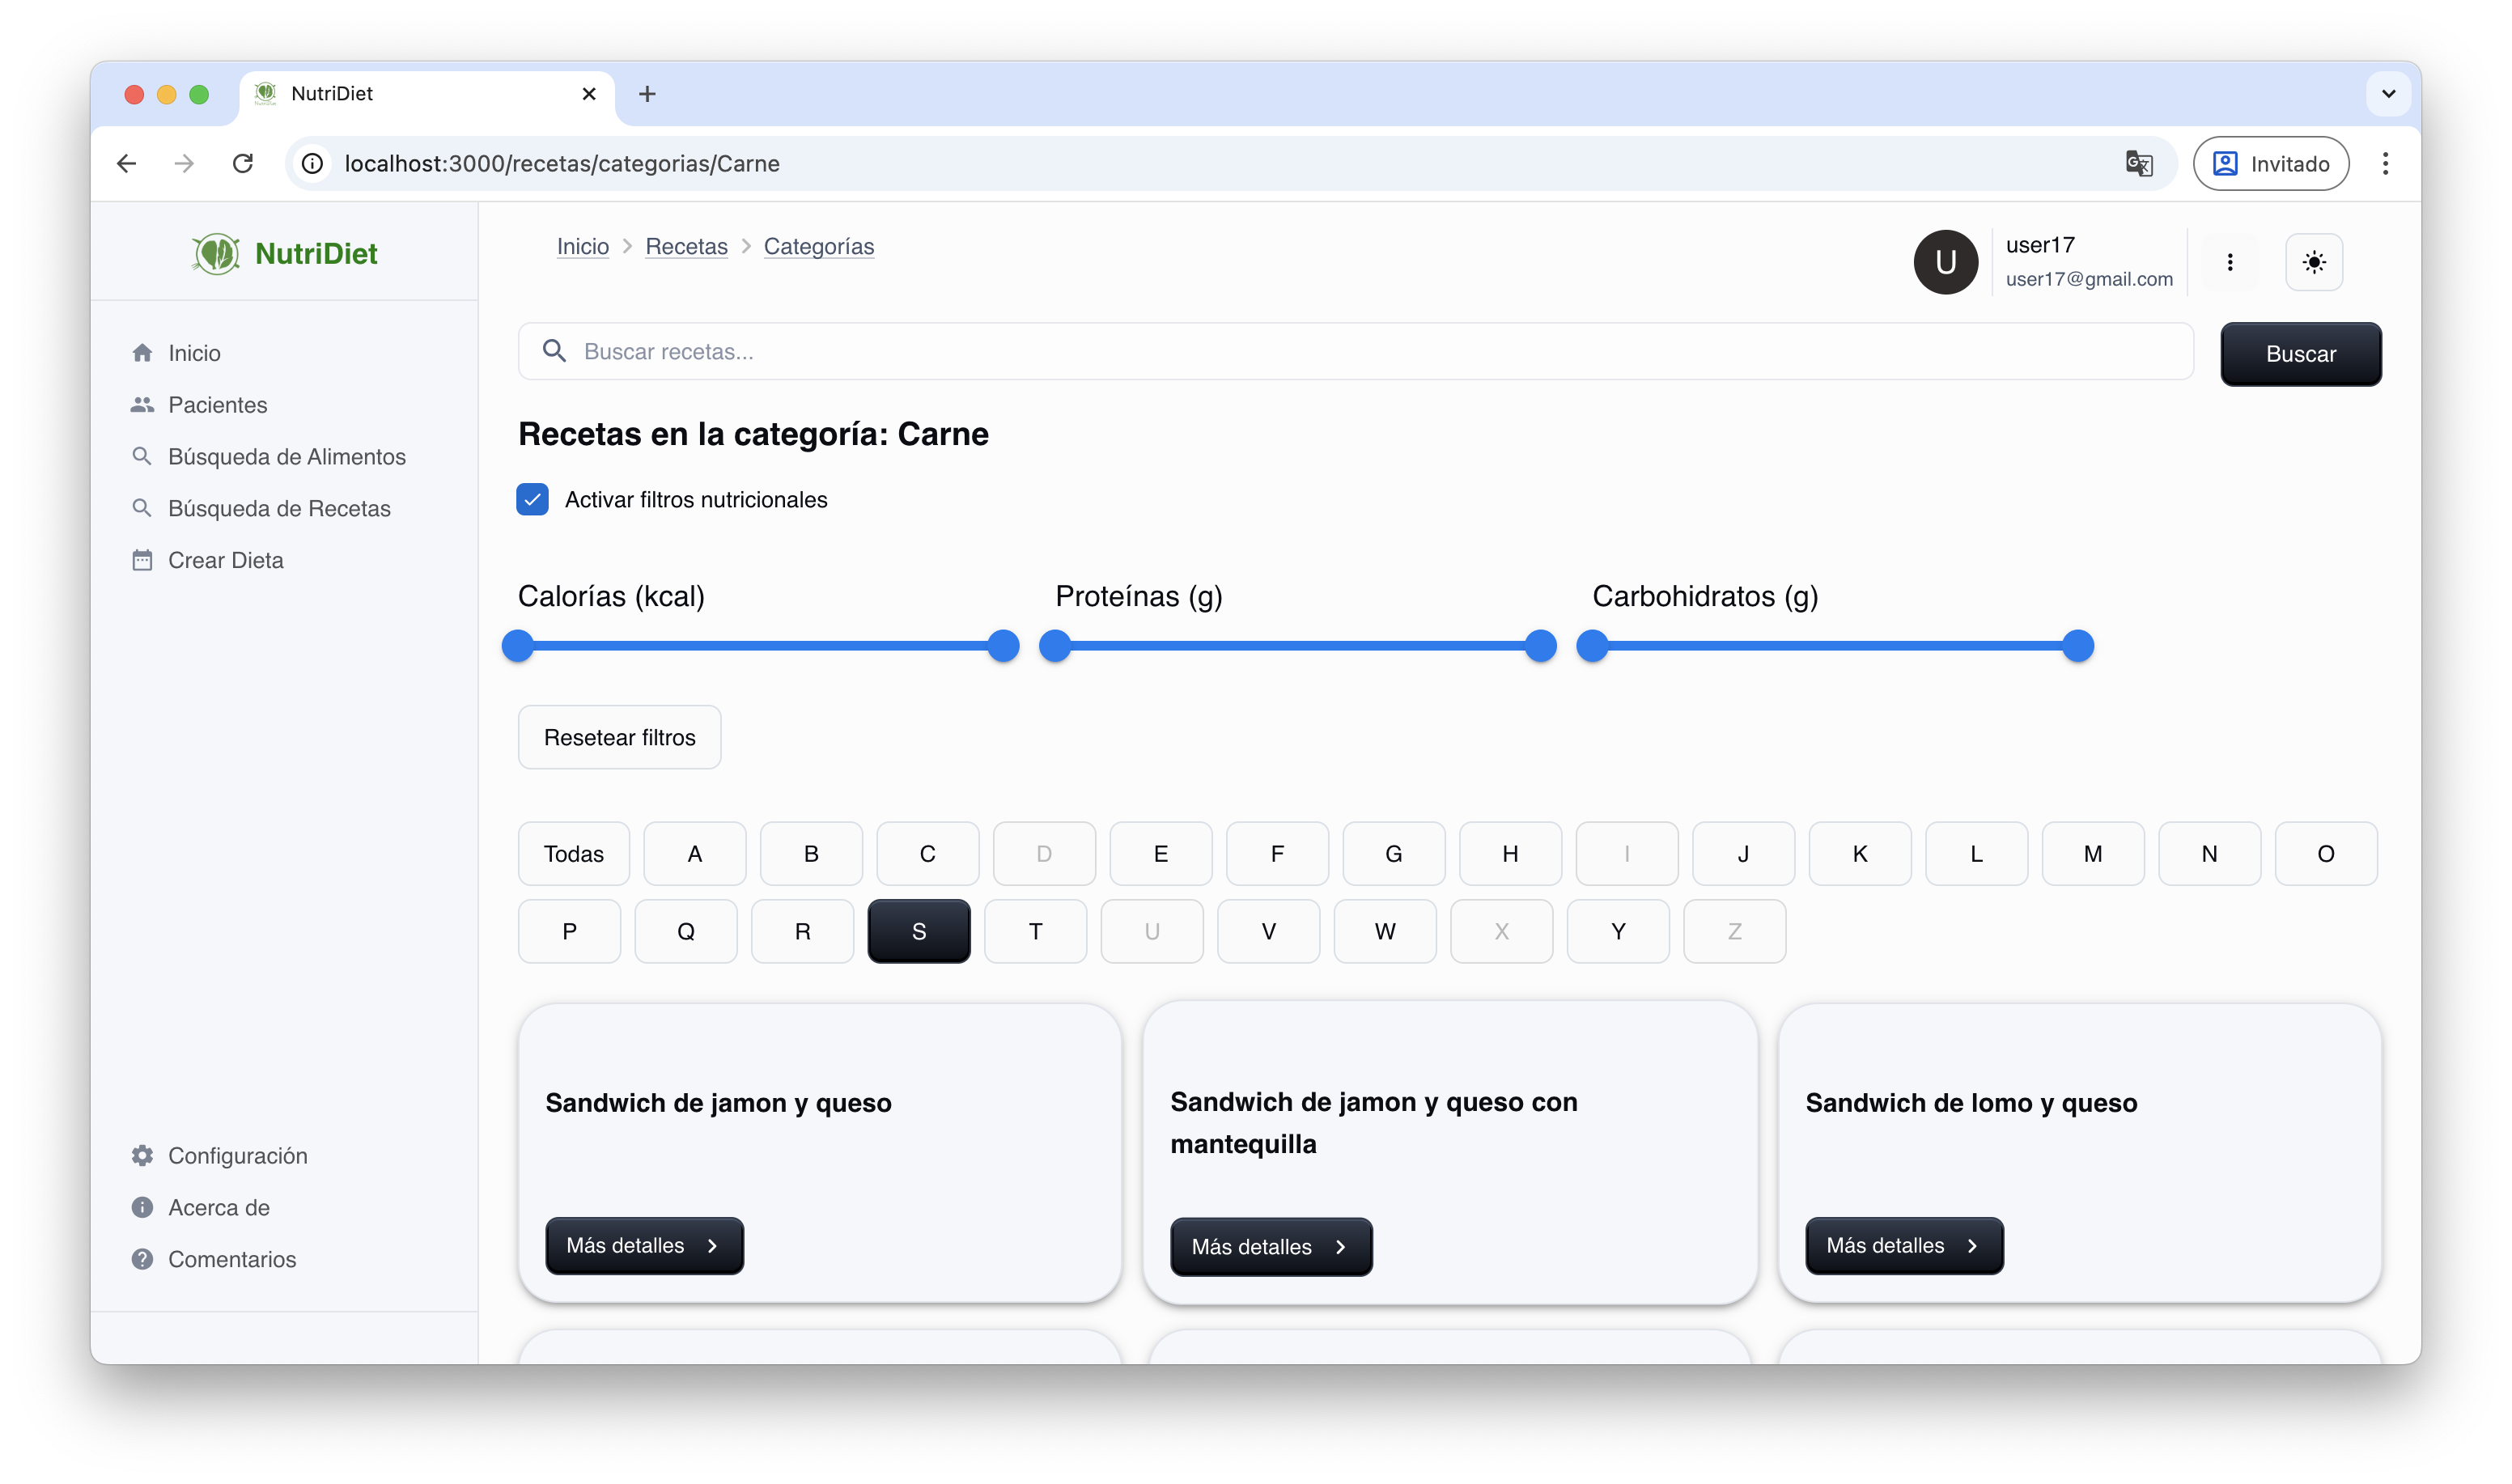
\includegraphics[width=1\linewidth]{Plantilla_TFG_latex//imagenes/Recetas_categoria.png}
    \caption{Vista de recetas filtradas por categoría con opciones de búsqueda y filtros nutricionales}
    \label{fig:Recetas_categoria}
\end{figure}


\subsection{Detalle de la receta}
La vista de detalle de una receta (Figura~\ref{fig:detalle-receta}) proporciona una descripción completa del plato, con información tanto culinaria como nutricional. En la parte superior se presenta el nombre de la receta acompañado de su categoría, país de origen, número de raciones y tiempo estimado de preparación. También se muestran etiquetas que identifican sus características dietéticas (por ejemplo: “Sin gluten”, “Bajo en grasa”) y su nivel de dificultad.

A continuación, se despliega el listado de ingredientes necesarios y los pasos detallados para su preparación. Ambos elementos están organizados en secciones colapsables que permiten una lectura cómoda y ordenada.

También tiene una tabla nutricional como los alimentos, que presenta los valores de energía, macronutrientes y micronutrientes por ración. Estos datos son calculados automáticamente a partir de los ingredientes vinculados a la receta y permiten evaluar el aporte nutricional del plato en relación con las necesidades diarias.

Además, se incluye un apartado con el comentario nutricional del profesional con fuente de origen, el cual ofrece observaciones relevantes sobre el perfil nutricional de la receta, posibles beneficios para la salud o recomendaciones para adaptar su consumo en diferentes tipos de dieta.

Finalmente, si existen otras recetas similares o relacionadas, se muestran como sugerencias para facilitar la navegación y fomentar la exploración de opciones alternativas dentro del sistema.

\begin{figure}[H]
    \centering
    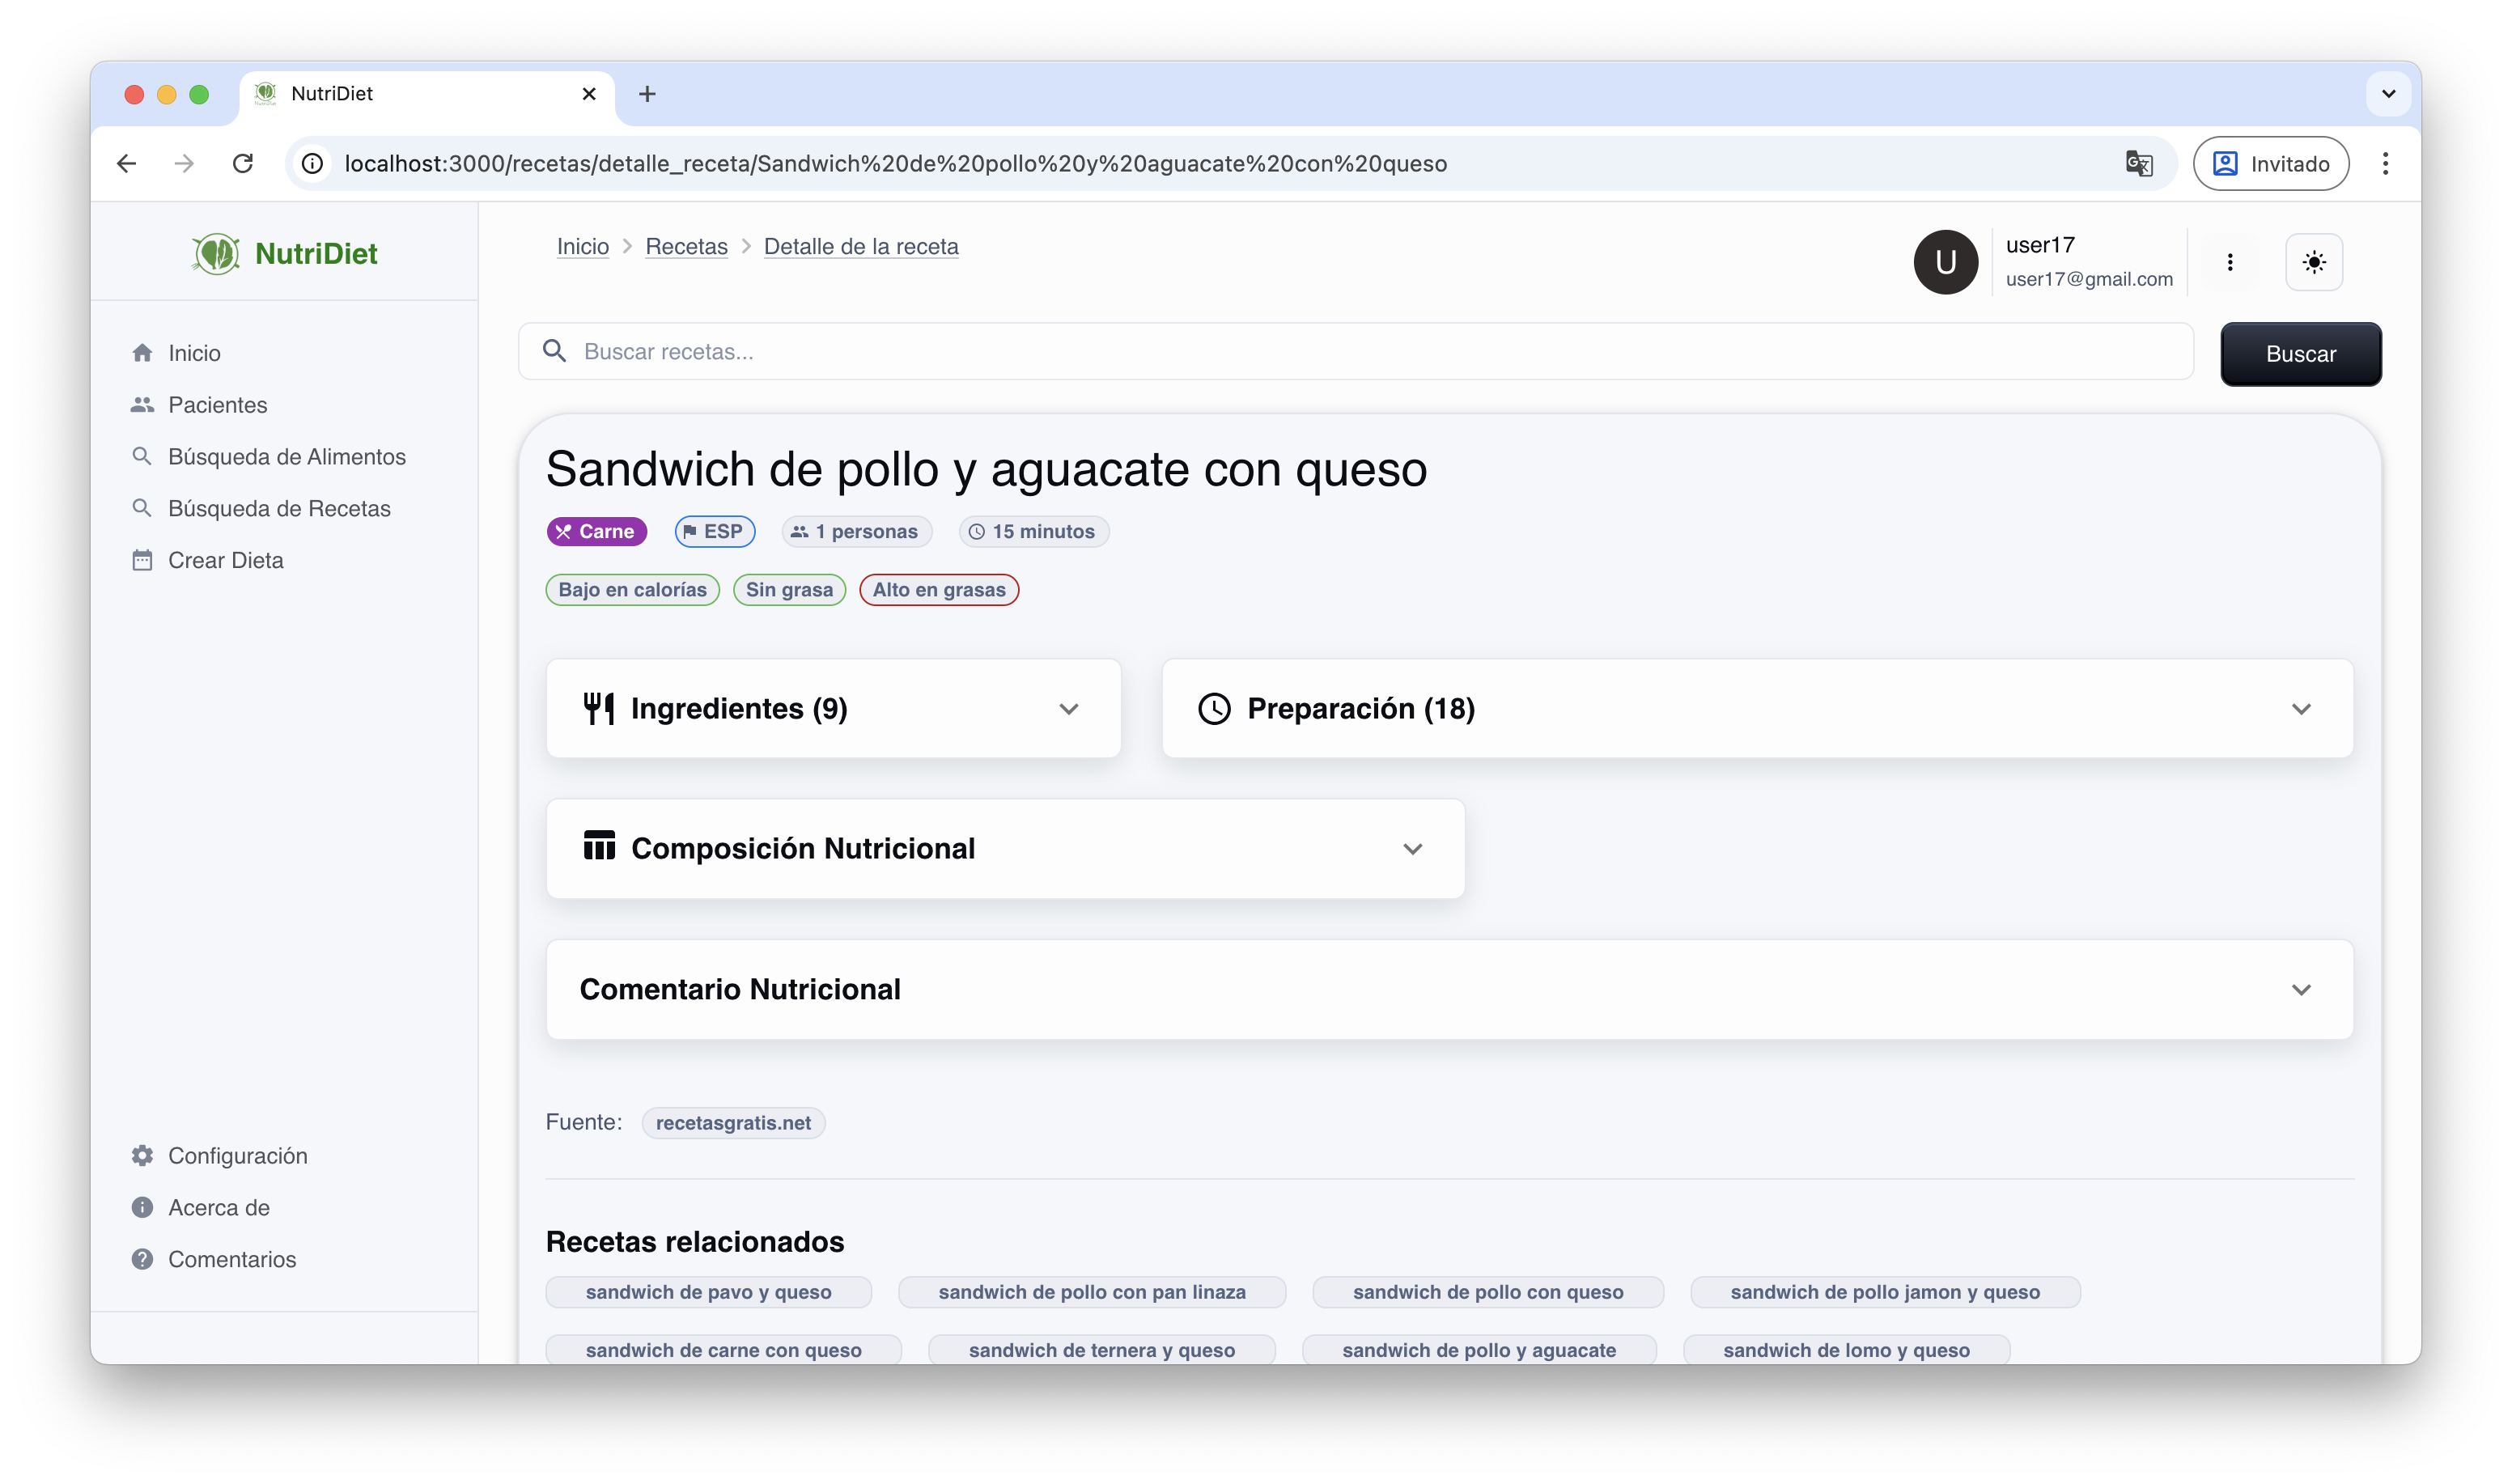
\includegraphics[width=1\linewidth]{Plantilla_TFG_latex//imagenes/Receta_detalle.png}
    \caption{Vista detallada de una receta con información nutricional, ingredientes, pasos de preparación y sugerencias relacionadas.}
    \label{fig:detalle-receta}
\end{figure}

\section{Planificación de dietas}
La funcionalidad de planificación de dietas (Figura~\ref{fig:PD_seleccionP}) permite al nutricionista diseñar, visualizar y gestionar menús estructurados para cada paciente a lo largo del tiempo. Una dieta está compuesta por un conjunto de días, y cada día incluye varias ingestas (por ejemplo: desayuno, almuerzo, cena), las cuales a su vez están formadas por recetas seleccionadas y clasificadas según el tipo de plato: entrante, primer plato, segundo plato, postre o bebida.

El proceso de planificación comienza seleccionando un paciente desde el panel correspondiente. Mientras no se haya seleccionado ningún paciente, el botón ``Continuar'' permanece deshabilitado (en gris) para evitar acciones prematuras. Este botón se habilita automáticamente y se muestra de forma destacada una vez que se ha elegido un paciente válido, guiando al nutricionista hacia el siguiente paso de la planificación. 

\begin{figure}[t]
    \centering
    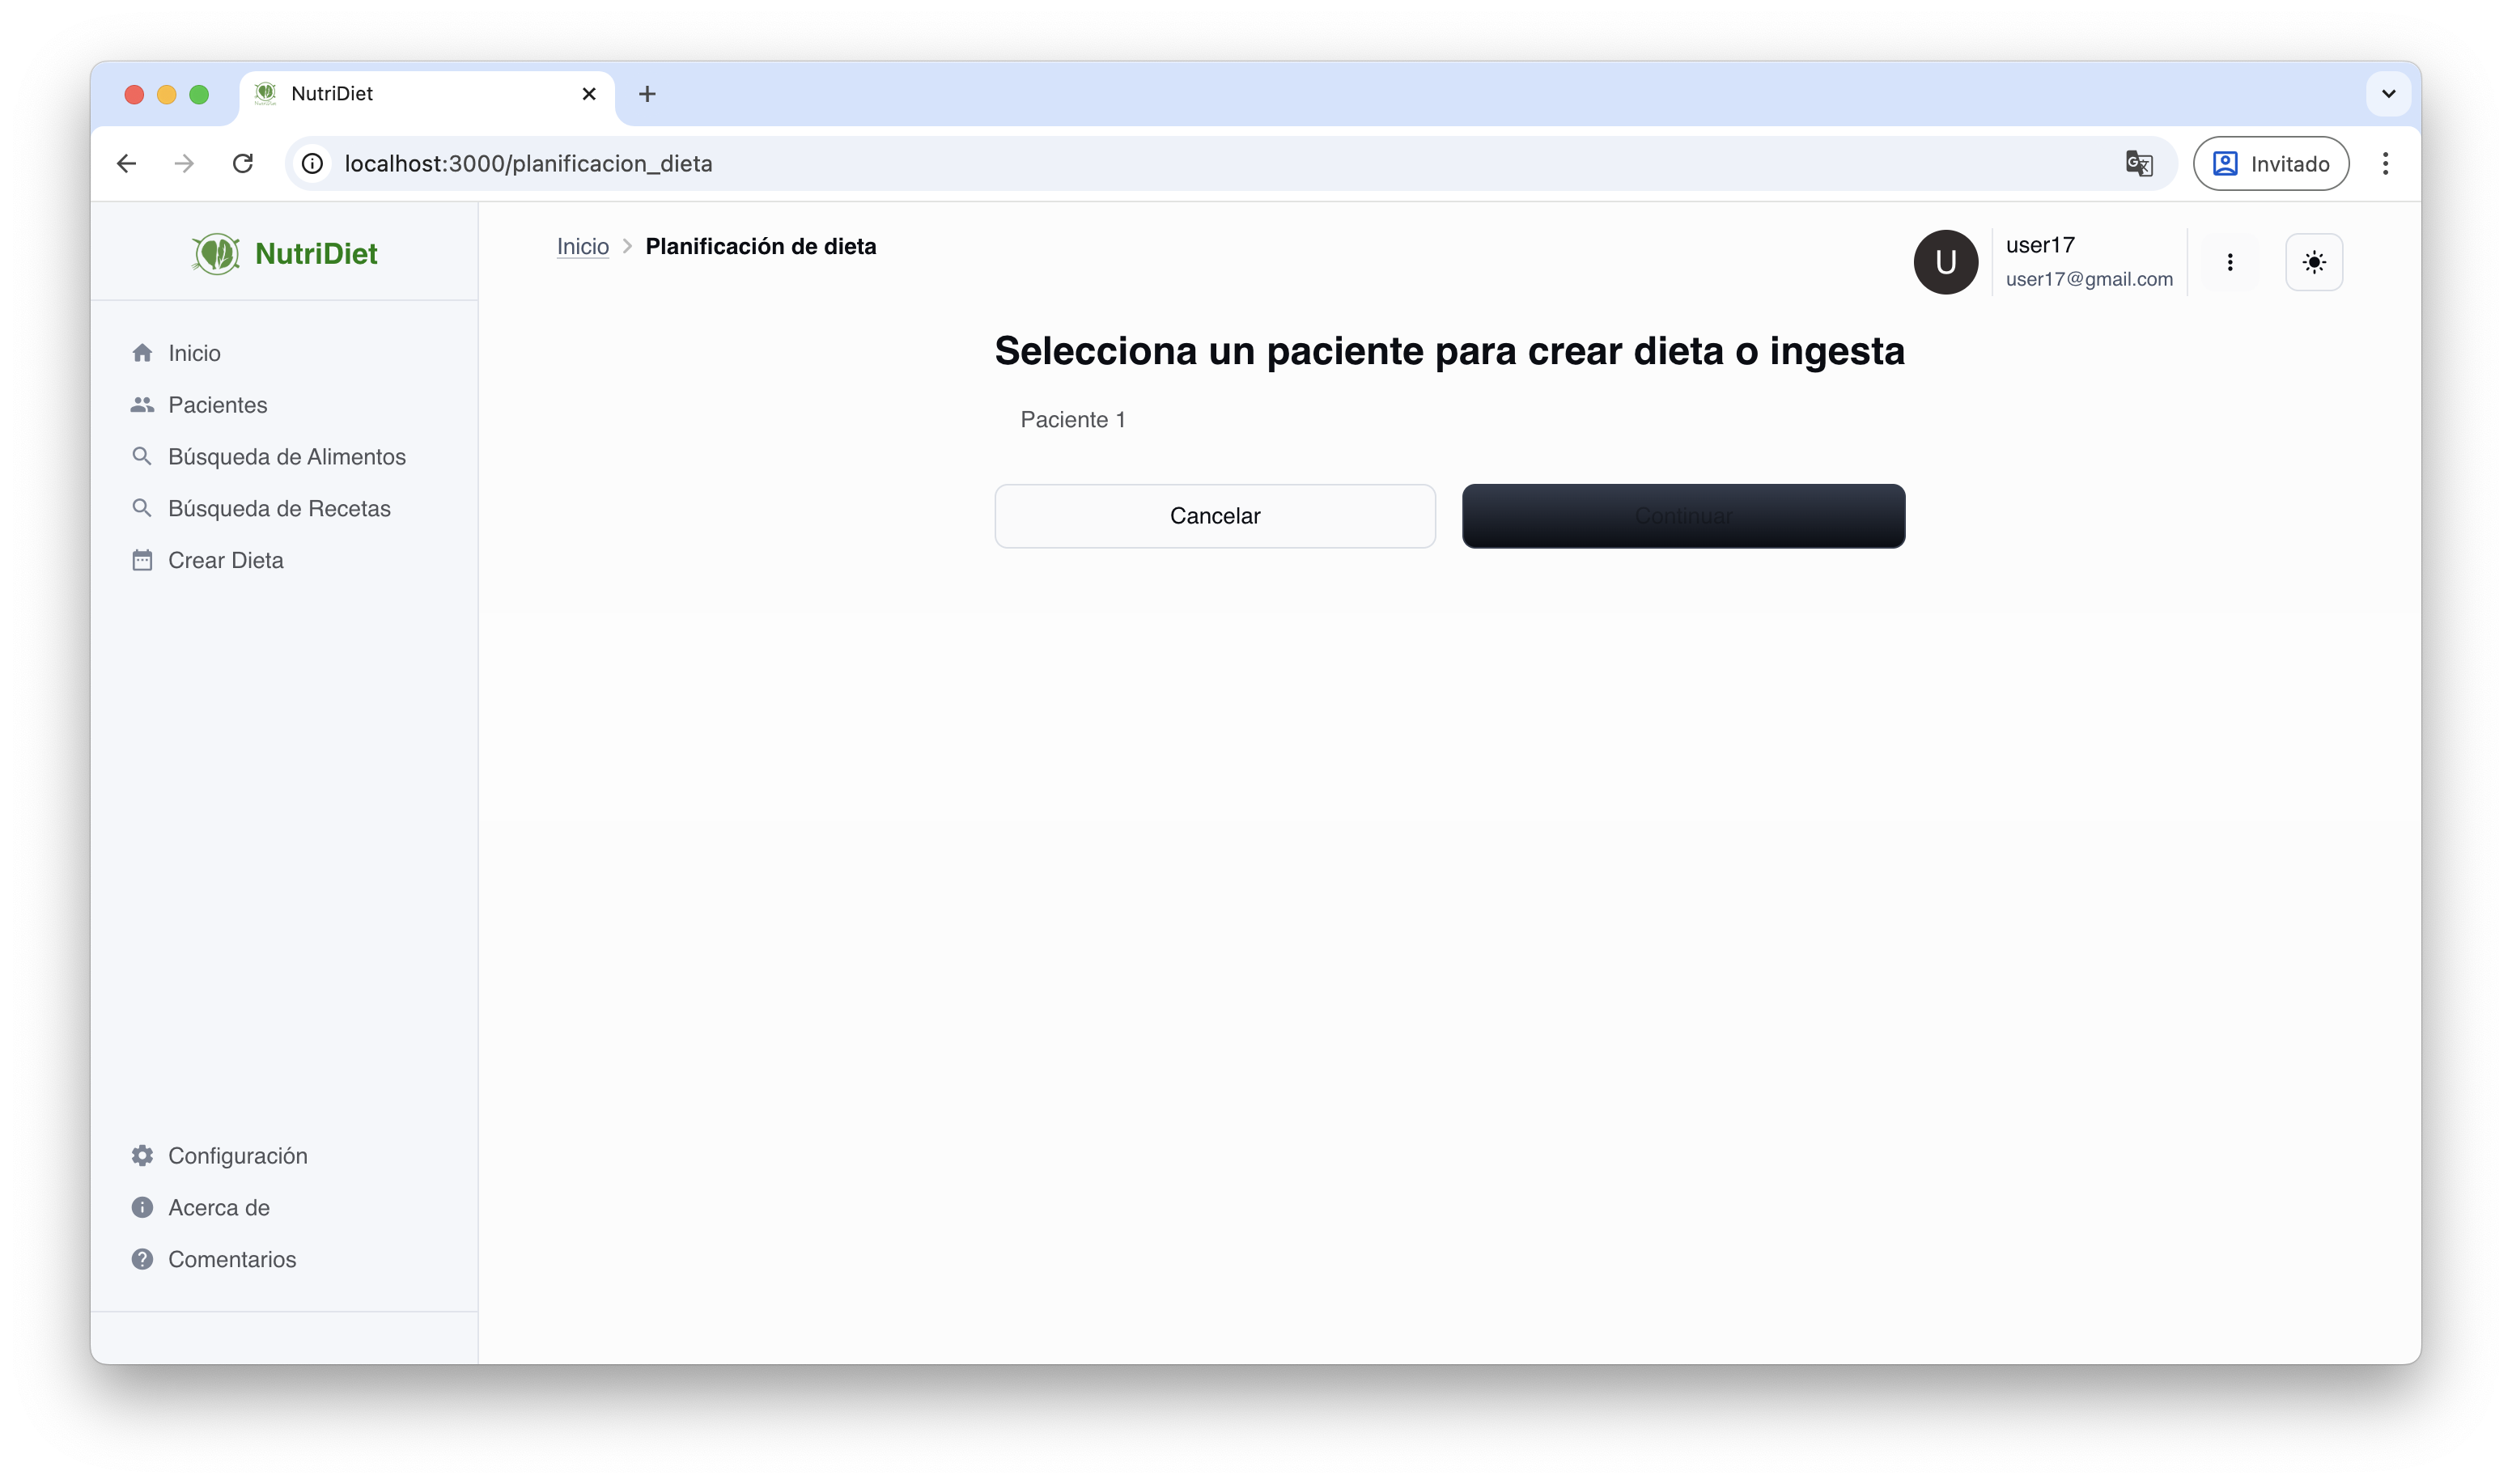
\includegraphics[width=1\linewidth]{Plantilla_TFG_latex//imagenes/PD_seleccionP.png}
    \caption{Vista de selección de paciente}
    \label{fig:PD_seleccionP}
\end{figure}

A partir de ahí, el sistema ofrece dos pestañas diferenciadas (Figura~\ref{fig:PD_ini}): una para gestionar dietas y otra para controlar las ingestas. Ambas vistas permiten crear, editar o eliminar elementos de manera independiente, manteniendo así un control granular sobre la planificación nutricional del paciente.

En la pestaña de ``Dietas'', el usuario puede:
\begin{itemize}
    \item Visualizar todas las dietas registradas del paciente, ordenadas por fecha.
    \item Aplicar filtros por año o por mes para localizar fácilmente las dietas de un periodo concreto.
    \item Identificar rápidamente la dieta activa, resaltada en un color distintivo respecto al resto.
    \item Acceder a los detalles de cada dieta mediante una tarjeta expandible, que muestra las fechas de inicio y fin, el número de días planificados y un resumen de ingestas por día.
    \item Funciones para crear una nueva dieta personalizada, editar/eliminar una dieta previa.
\end{itemize}

En la pestaña de ``Ingestas'', se ofrece un listado de todas las ingestas individuales asignadas al paciente. Esta sección incluye:
\begin{itemize}
    \item Filtros por tipo de ingesta (desayuno, media mañana, almuerzo, merienda, cena) para facilitar la navegación.
    \item Tarjetas con diseño plegable que revelan información específica al expandirse: nombre de la ingesta, recetas incluidas clasificadas por tipo de plato, comentarios nutricionales y número de raciones.
    \item Funciones para crear una nueva ingesta personalizada, reutilizar una ingesta existente o editar/eliminar una previa.
\end{itemize}

\begin{figure}[H]
    \centering
    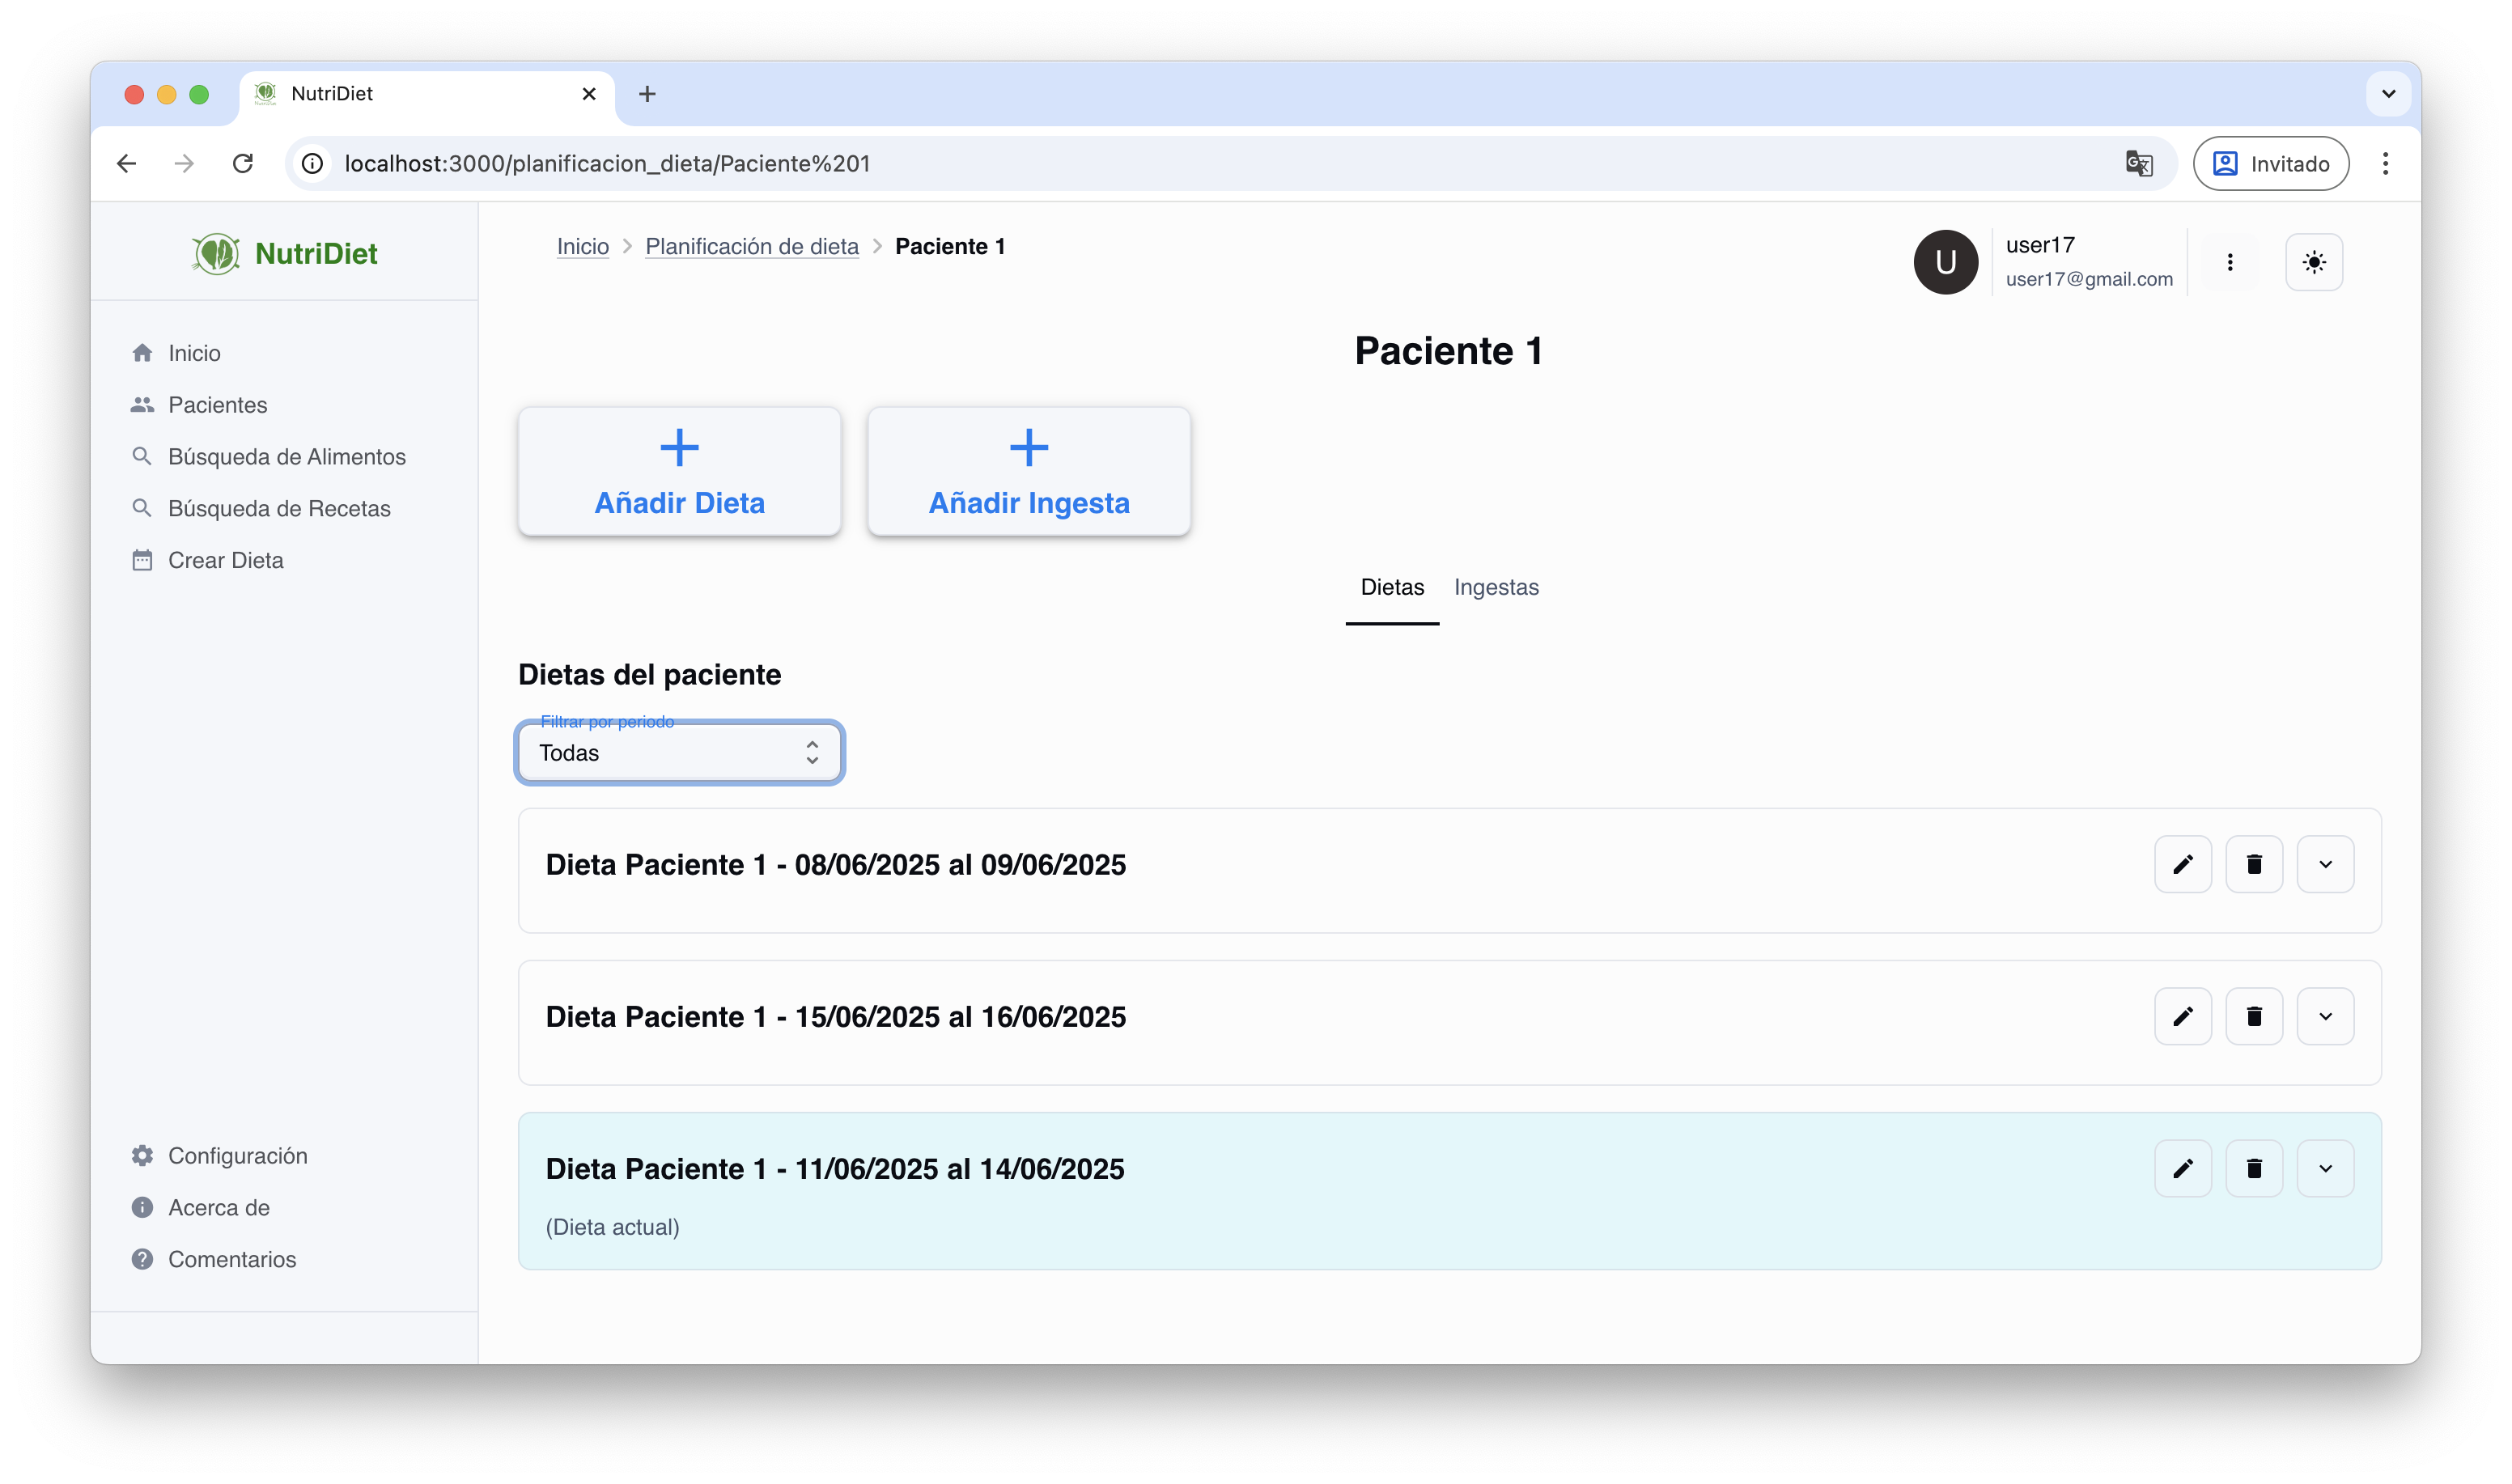
\includegraphics[width=1\linewidth]{Plantilla_TFG_latex//imagenes/PD_ini.png}
    \caption{Vista de planificación de dietas con pestañas para dietas e ingestas}
    \label{fig:PD_ini}
\end{figure}

\subsection{Crear ingesta}
El sistema permite crear una ingesta personalizada para un paciente concreto o ingestas universales que pueden ser utilizadas por todos los pacientes, especificando el nombre de la ingesta, el tipo de comida (por ejemplo: desayuno, almuerzo, cena) y las recetas que la componen, clasificadas según su función dentro del menú (entrante, primer plato, segundo plato, postre o bebida).

El proceso de creación comienza con un formulario (Figura~\ref{fig:crear-ingesta-form}) donde se debe introducir el nombre de la ingesta y seleccionar el tipo correspondiente. Esta información inicial es obligatoria para continuar con el diseño del contenido.

\begin{figure}[t]
    \centering
    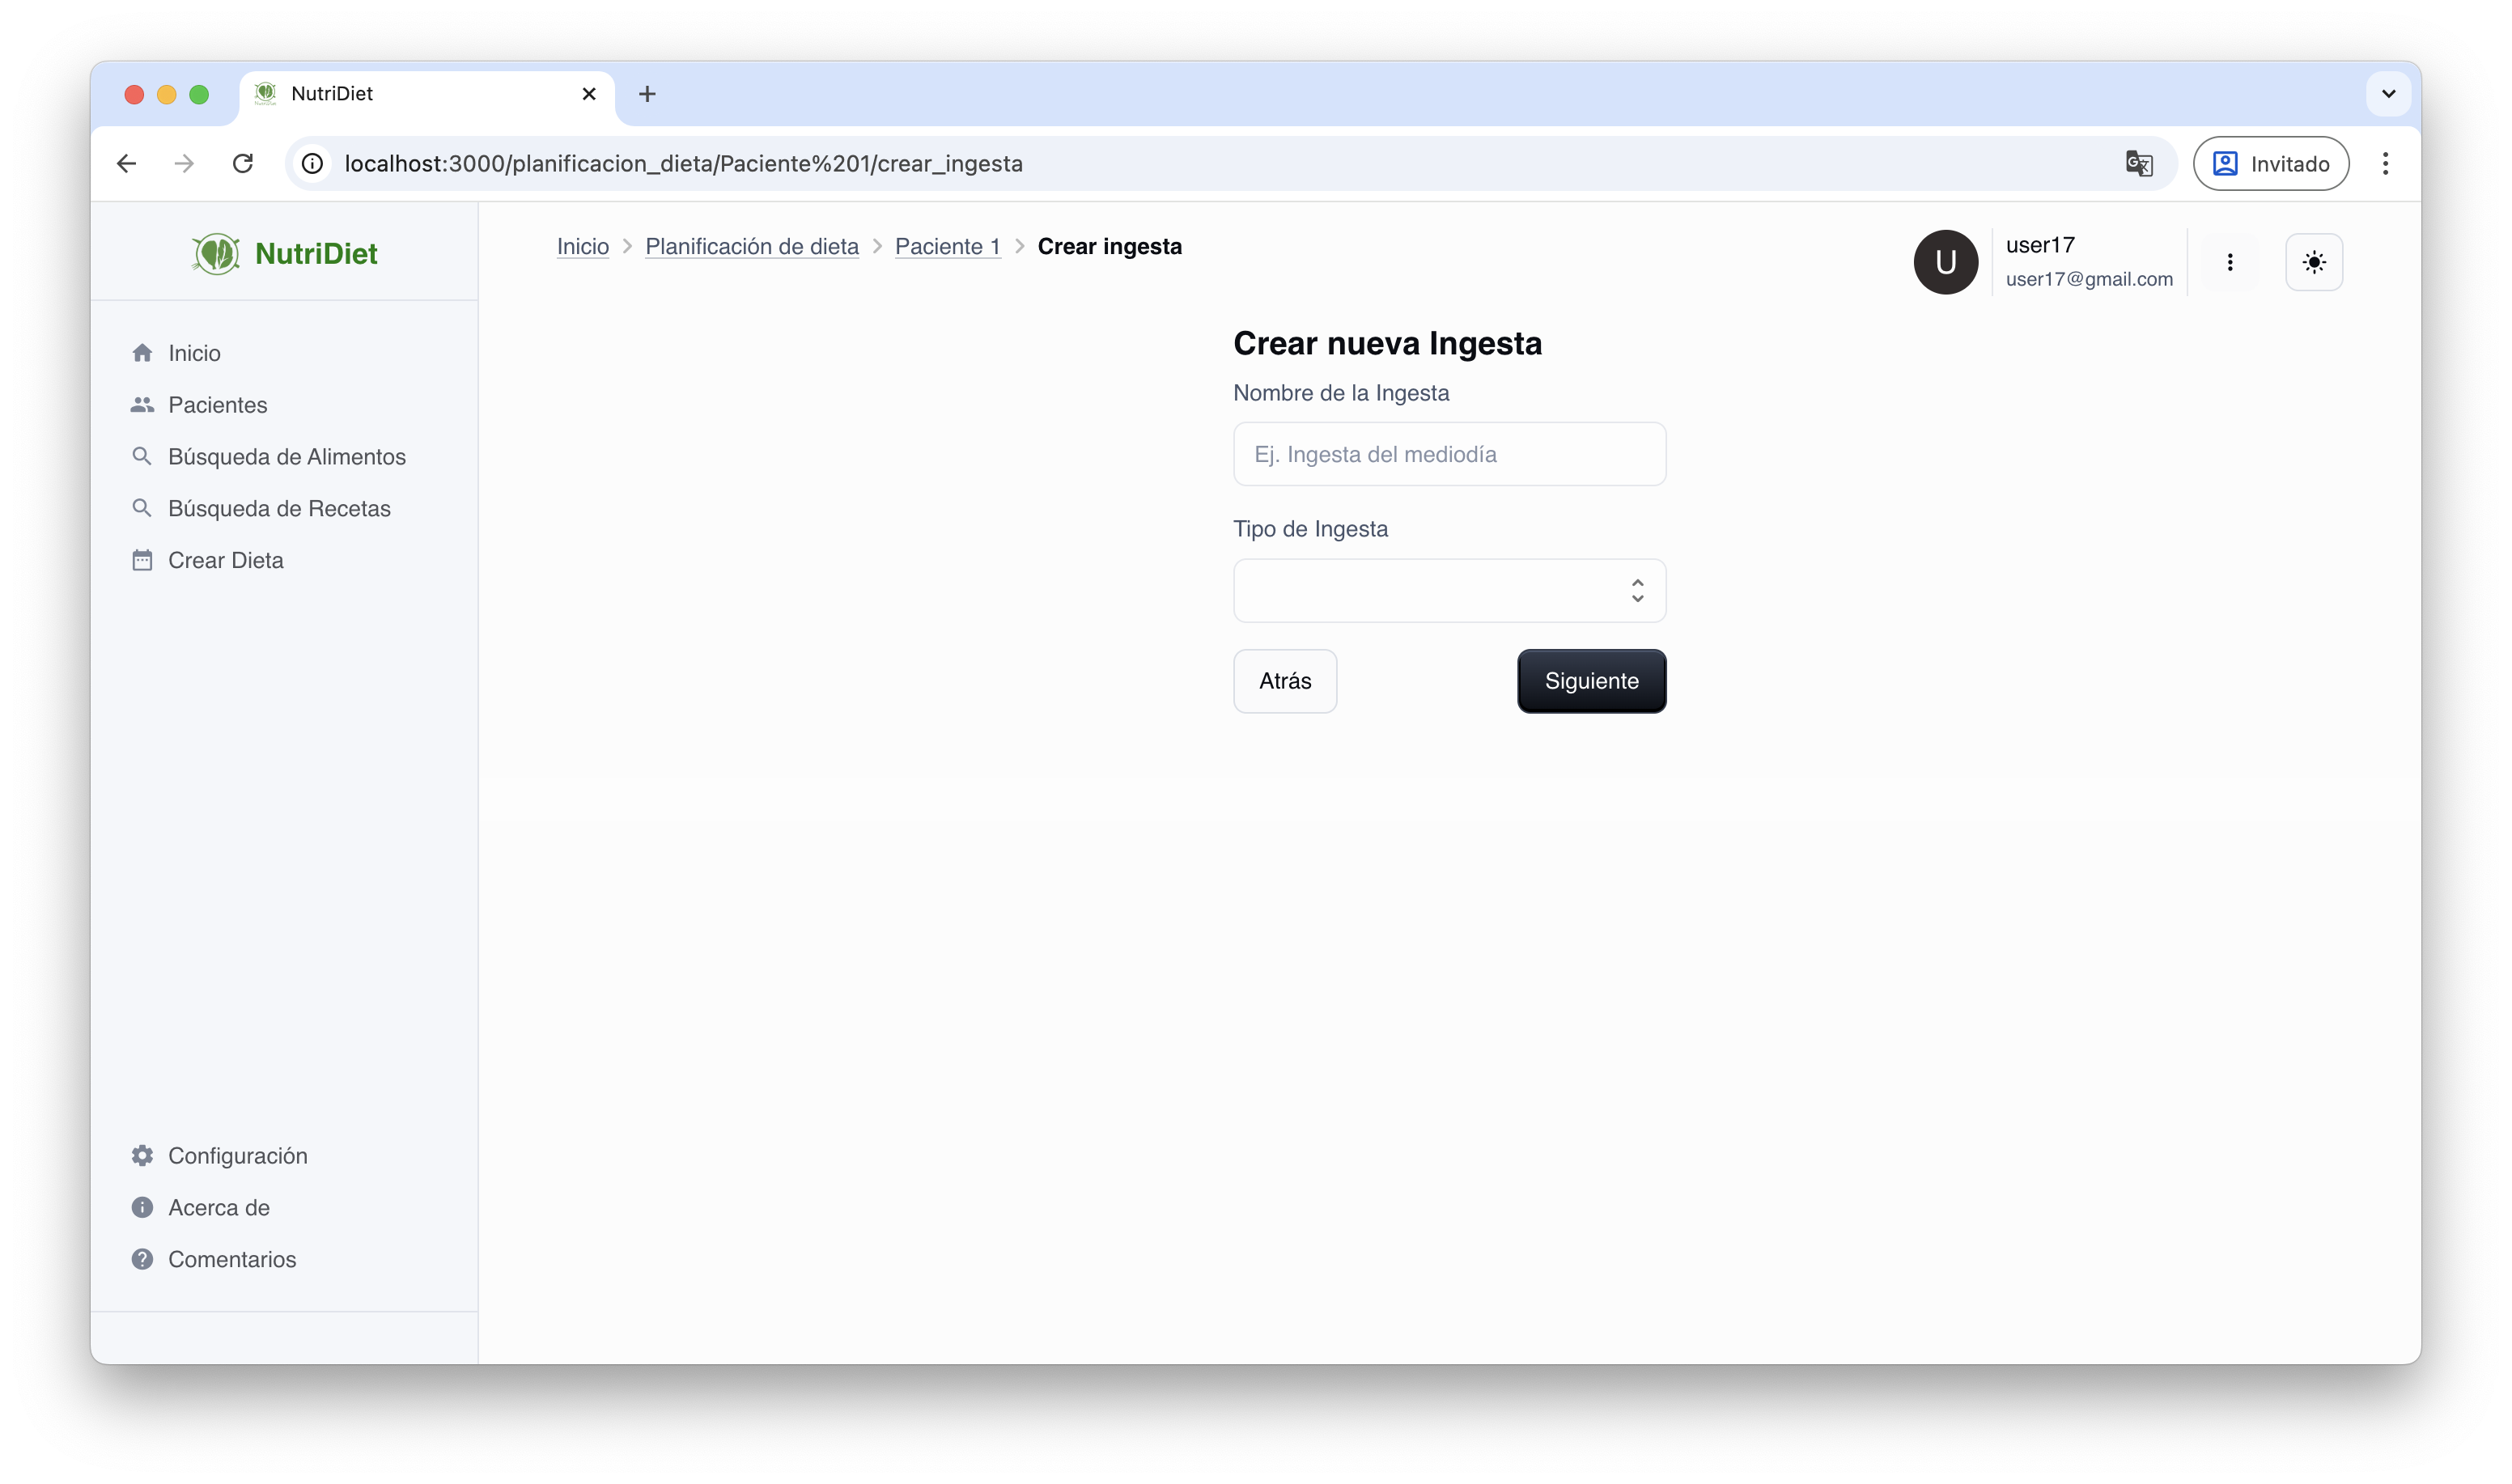
\includegraphics[width=1\linewidth]{Plantilla_TFG_latex/imagenes/PD_crearIngestaN.png}
    \caption{Formulario inicial de creación de una nueva ingesta: nombre y tipo de comida.}
    \label{fig:crear-ingesta-form}
\end{figure}

Una vez seleccionado el tipo de ingesta, el sistema muestra de forma visual (Figura~\ref{fig:crear-ingesta-drag}) los requerimientos nutricionales diarios esperados para dicha comida, calculados en función del total diario recomendado al paciente. Estos valores incluyen calorías, proteínas y carbohidratos estimados como objetivo para esa fracción del día.

Junto al nombre de la ingesta y los valores absolutos de referencia, se presenta un panel comparativo que muestra cuánto se ha cubierto con las recetas seleccionadas. Este panel utiliza indicadores circulares que reflejan el porcentaje alcanzado de cada macronutriente respecto al objetivo marcado.

\begin{itemize}
    \item Nombre de la ingesta: aparece destacado en la parte superior del panel.
    \item Objetivo nutricional: se indican los valores en kilocalorías, gramos de proteína y carbohidratos que deberían alcanzarse según el tipo de ingesta (por ejemplo, un 30\% del total diario en un almuerzo).
    \item Porcentaje alcanzado: mediante gráficos circulares, se visualiza el progreso real conforme se añaden recetas, lo que ayuda a equilibrar la composición nutricional de la ingesta.
\end{itemize}

Esta funcionalidad permite al profesional tener una visión inmediata del grado de adecuación de la ingesta a los requerimientos establecidos, facilitando ajustes antes de guardar o aplicar la planificación.

Por debajo está la interfaz interactiva basada en el sistema de ``drag-and-drop'', donde el usuario puede buscar recetas por nombre o por categoría y arrastrarlas directamente a las zonas correspondientes según el tipo de plato. Esta organización por zonas facilita la estructuración lógica del menú. La búsqueda de recetas también permite aplicar filtros nutricionales como calorías, proteínas y carbohidratos, lo que permite crear ingestas adaptadas a diferentes objetivos dietéticos.

Cada bloque de tipo de plato puede contener una o varias recetas, y el sistema muestra visualmente cuántas se han asignado a cada uno. Además, existe la opción de marcar una ingesta como ``universal'', lo cual indica que puede ser reutilizada para diferentes pacientes.

Una vez completada la planificación, el usuario puede guardar la ingesta, la cual queda registrada y disponible para su uso posterior dentro del sistema de planificación de dietas.

\begin{figure}[t]
    \centering
    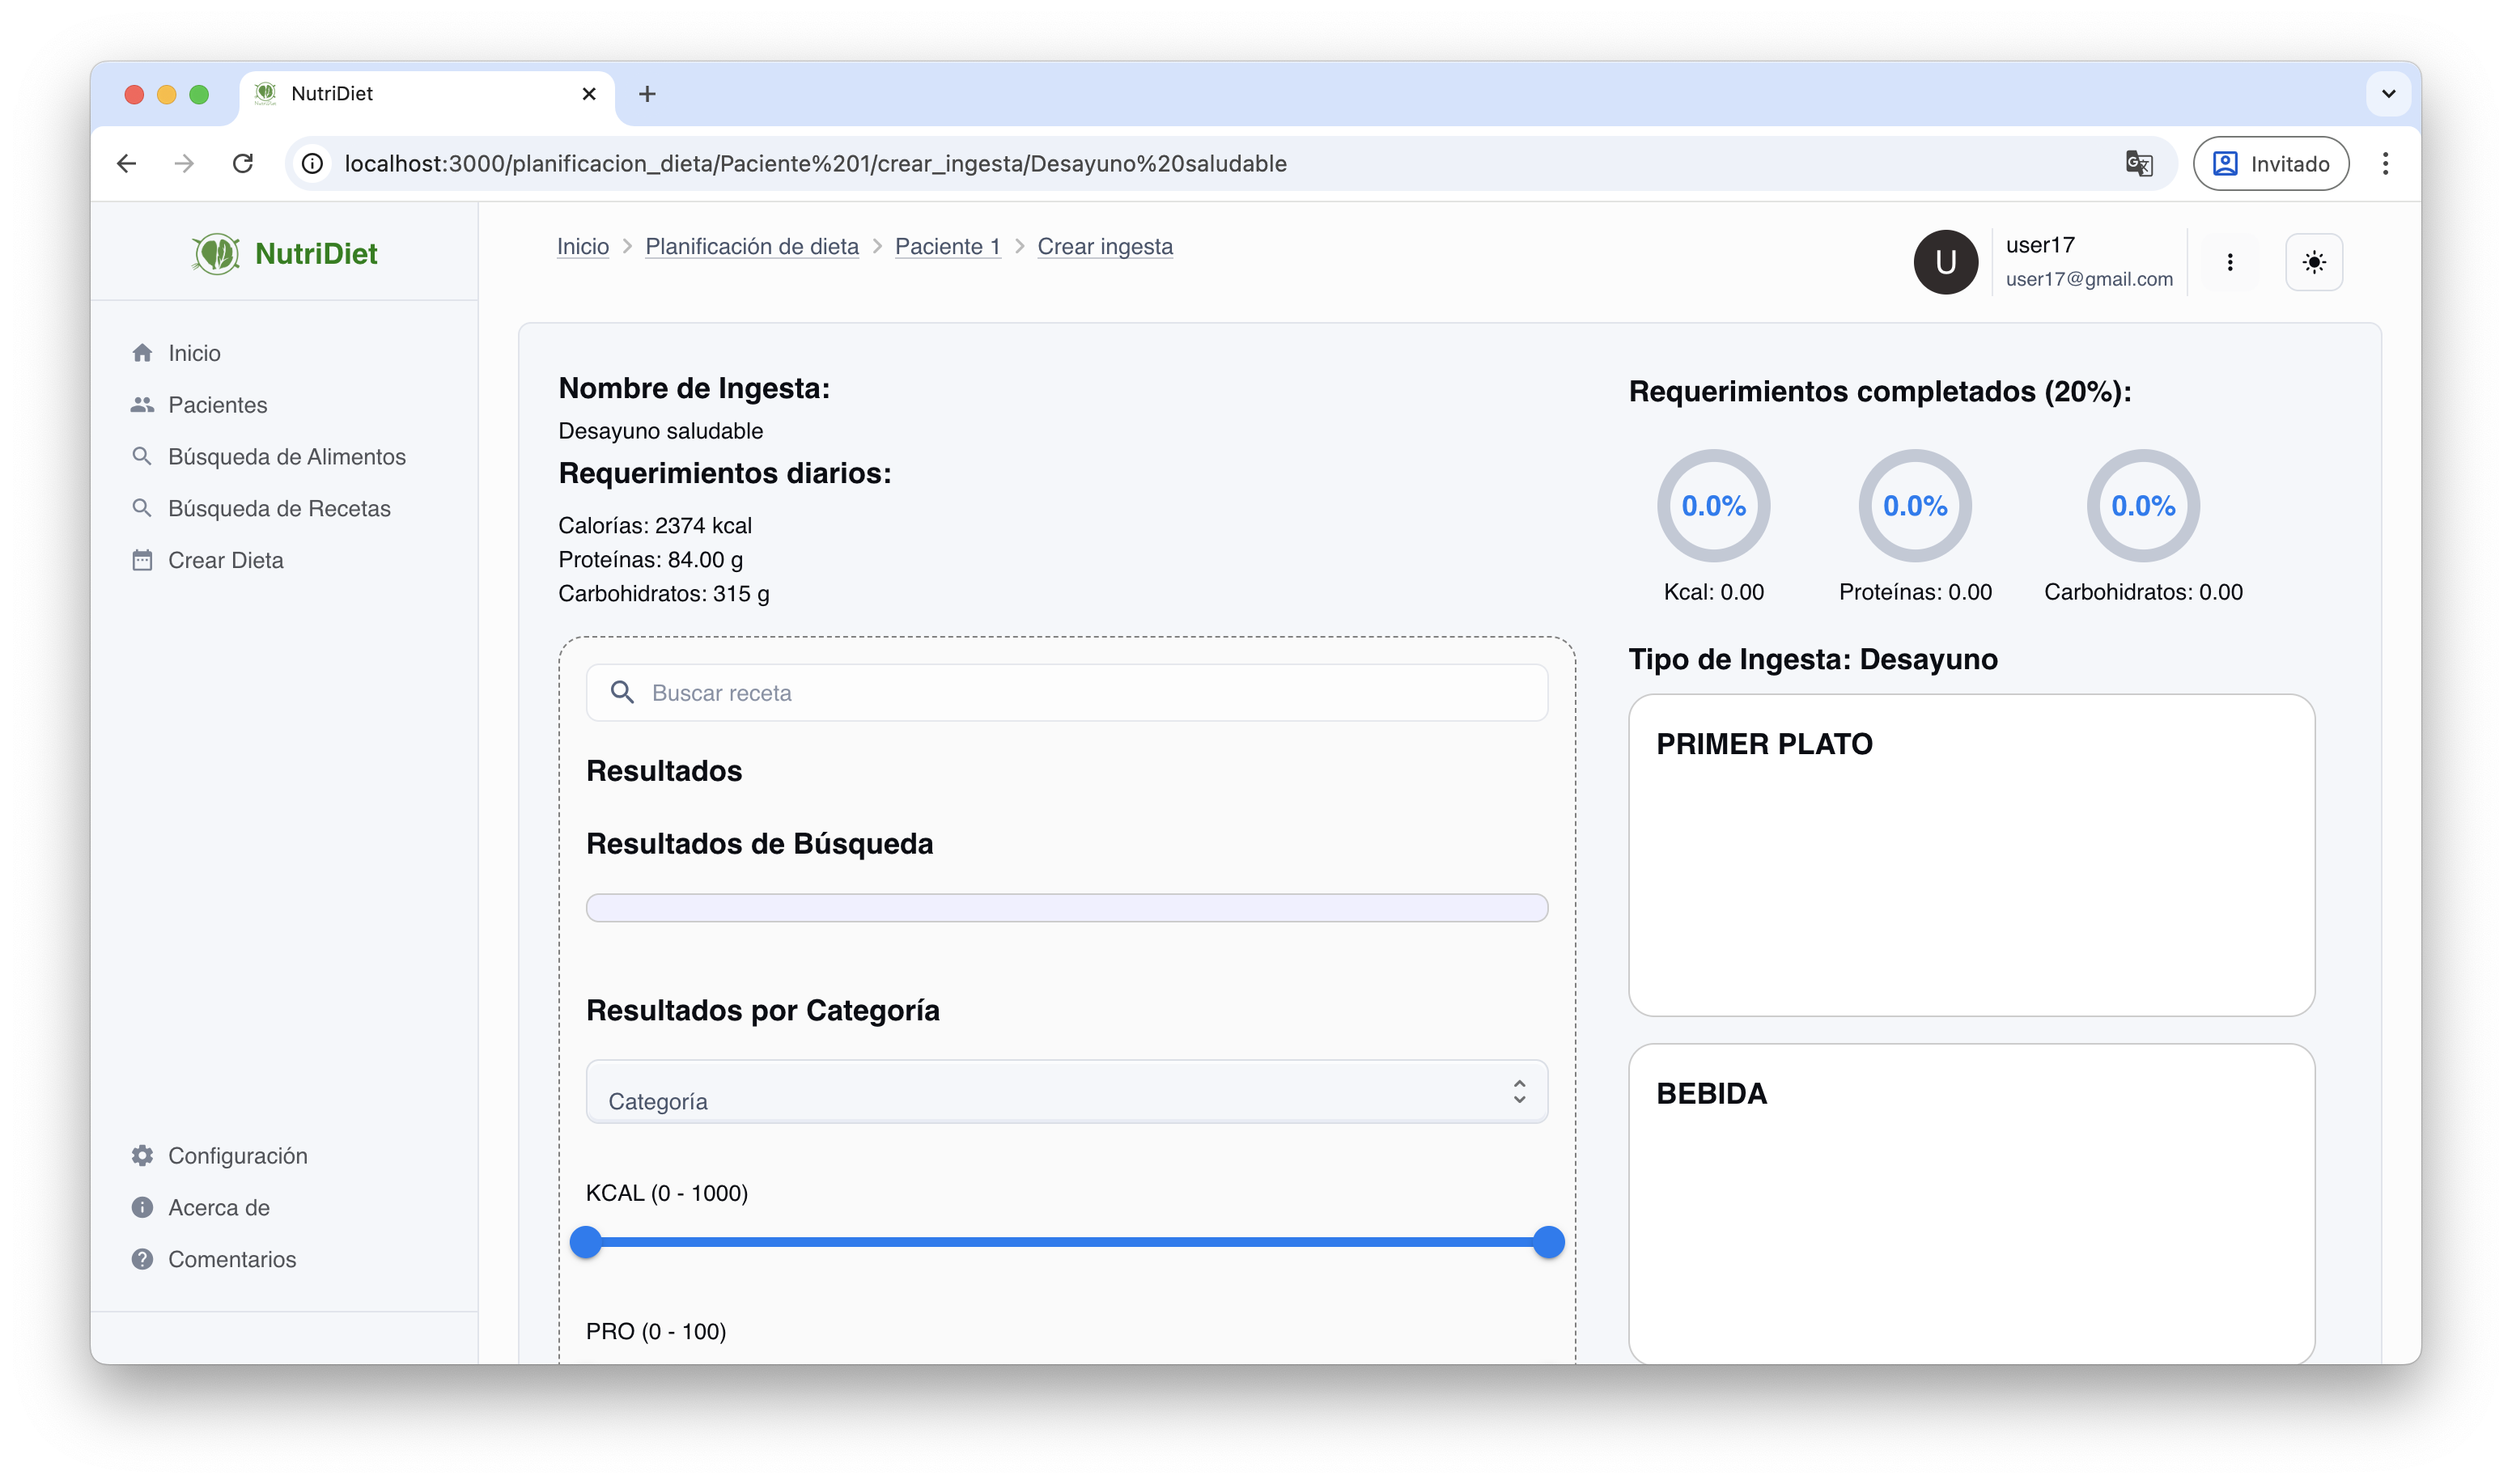
\includegraphics[width=1\linewidth]{Plantilla_TFG_latex//imagenes/PD_crearIngesta.png}
    \caption{Vista de arrastre de recetas a los bloques correspondientes por tipo de plato con requerimiento de nutrición esencial.}
    \label{fig:crear-ingesta-drag}
\end{figure}

\subsection{Crear dieta}
La creación de una dieta permite al profesional definir un plan nutricional estructurado para un paciente durante un intervalo de fechas concreto. 
Cada día del plan puede incluir una o varias ingestas ya existentes, o nuevas que se crean en el momento, asegurando así una planificación flexible y personalizada.

El proceso de creación comienza con la selección de un rango de fechas (Figura~\ref{fig:crear-dieta-form}). Una vez definido el periodo de planificación, el sistema muestra los requerimientos nutricionales diarios del paciente (calorías, proteínas, carbohidratos), como referencia para evaluar si la dieta está balanceada globalmente.

\begin{figure}
    \centering
    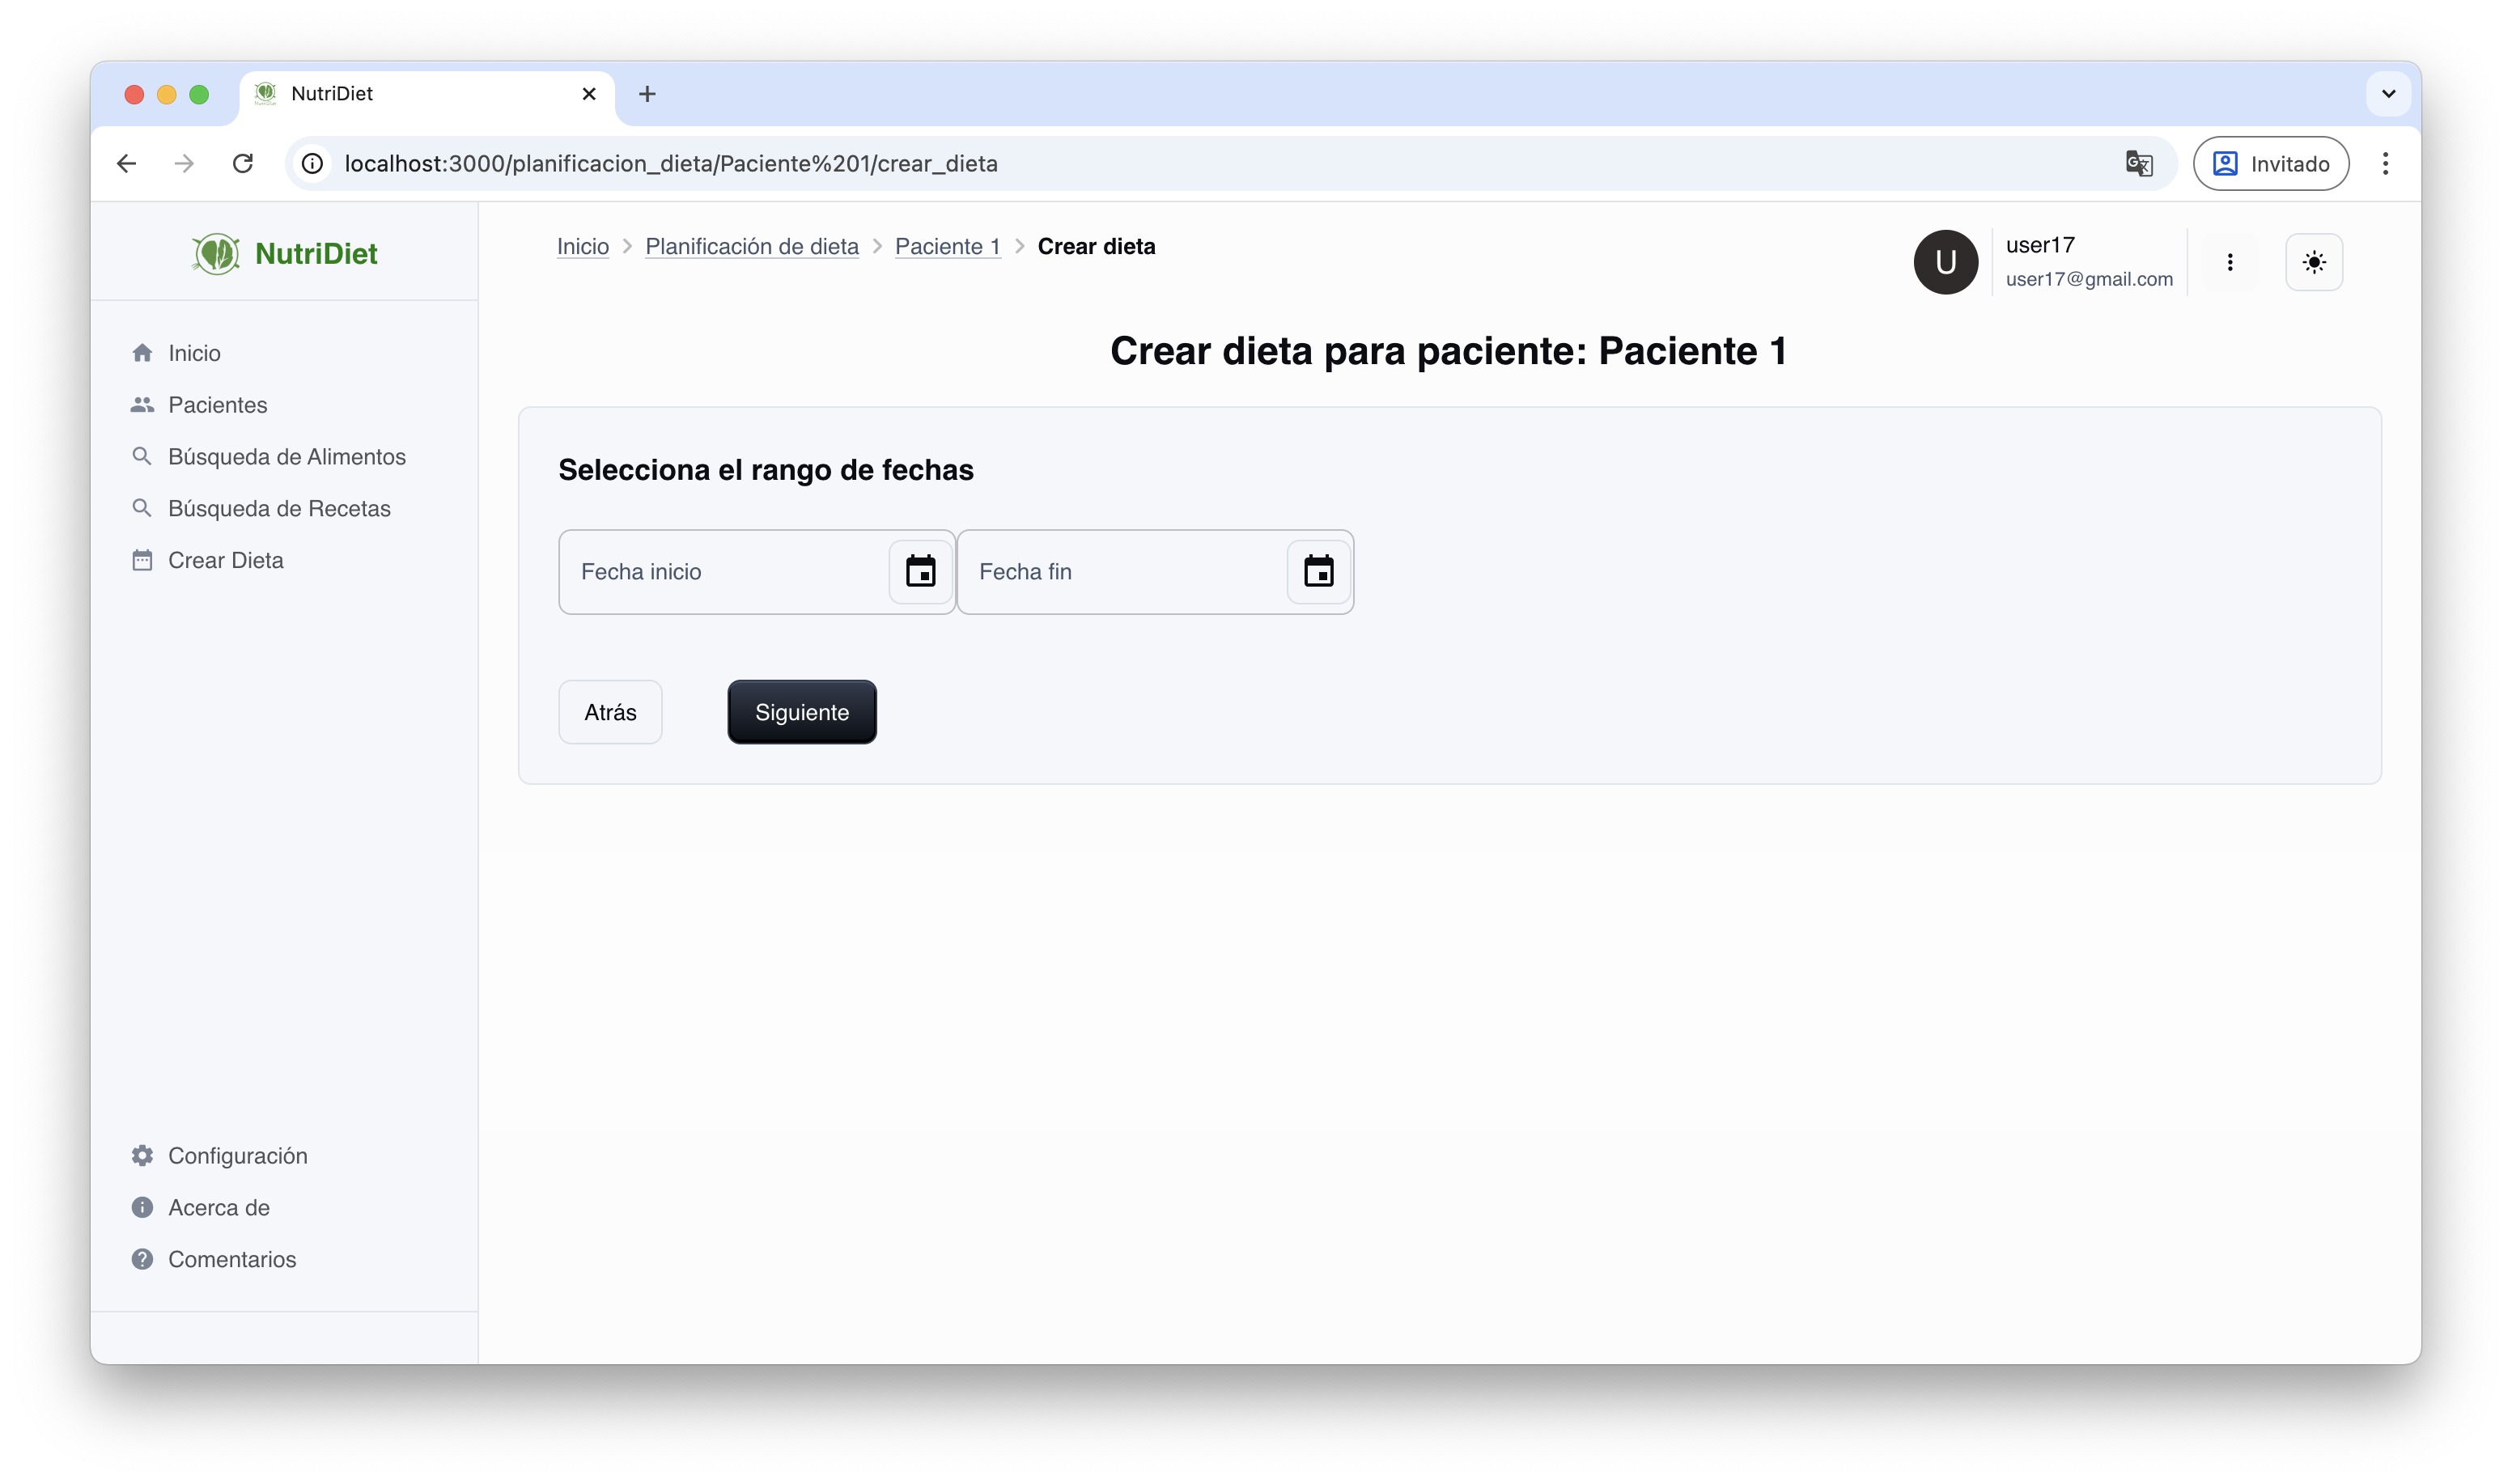
\includegraphics[width=1\linewidth]{Plantilla_TFG_latex//imagenes/PD_creardieta.png}
    \caption{Formulario inicial para crear una nueva dieta: selección de fechas.}
    \label{fig:crear-dieta-form}
\end{figure}

La interfaz (Figura~\ref{fig:crear-dieta-plan}) se compone de dos secciones principales:

\begin{figure}
    \centering
    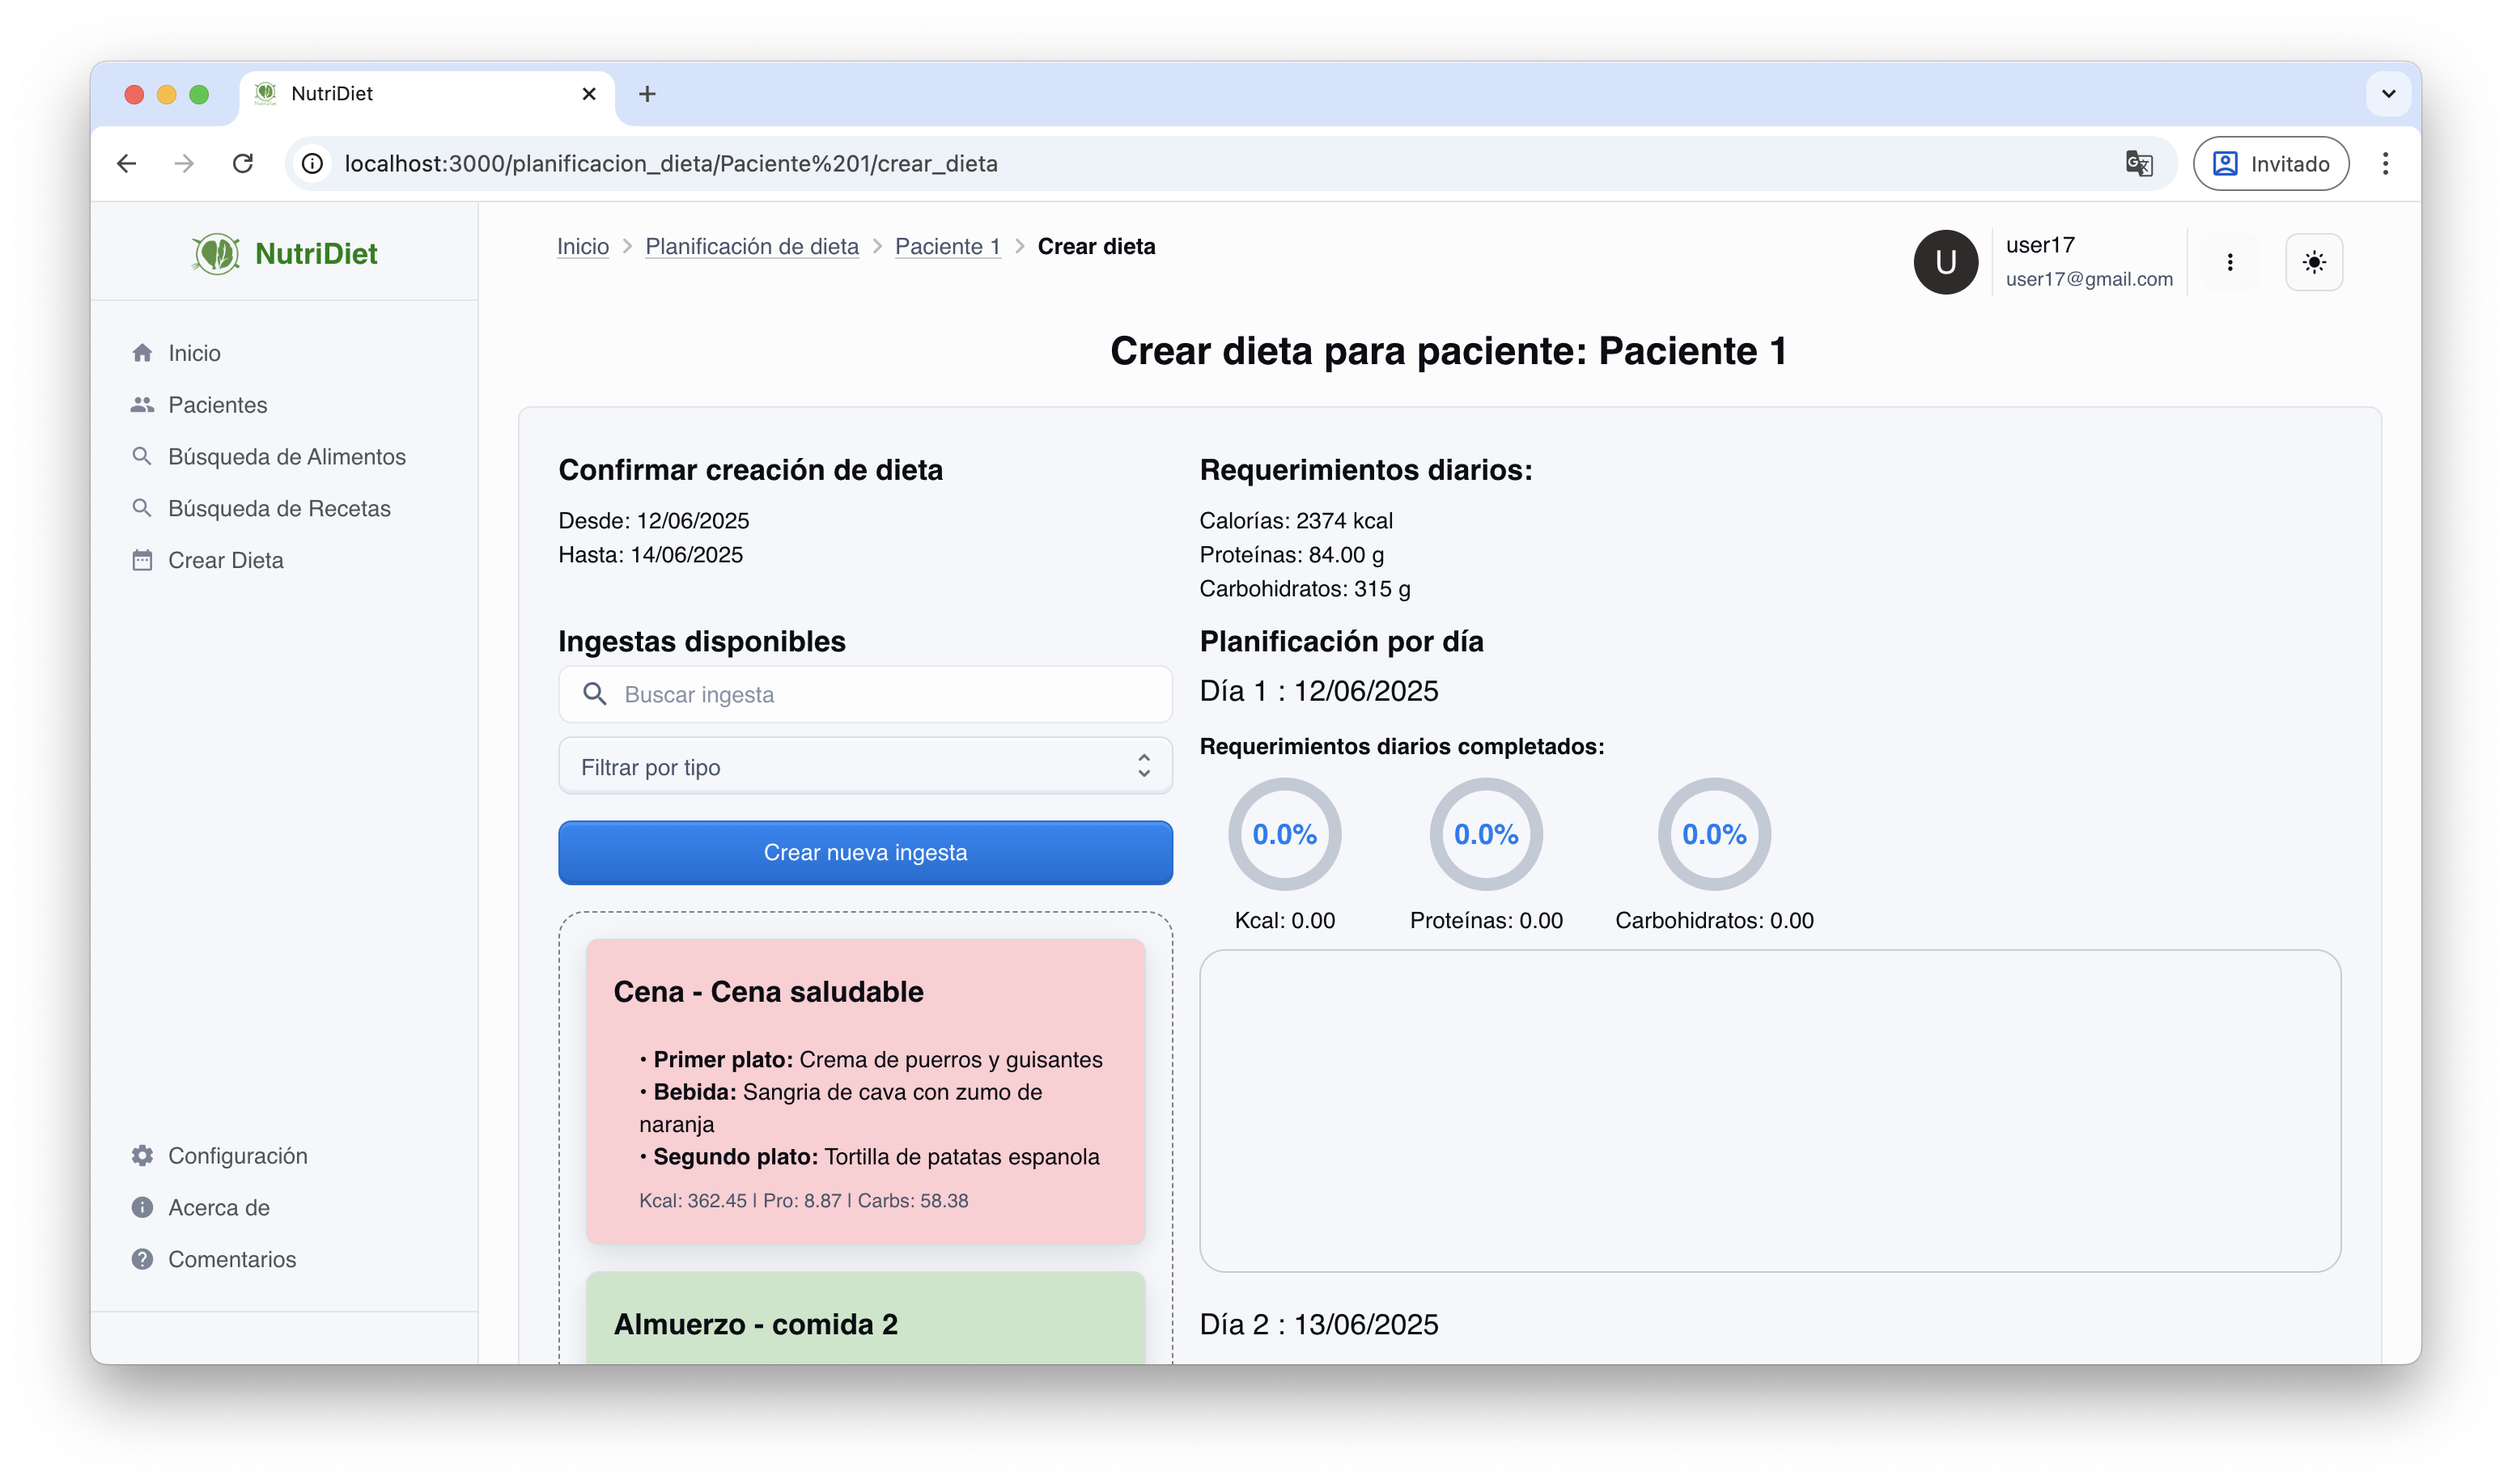
\includegraphics[width=1\linewidth]{Plantilla_TFG_latex//imagenes/PD_crearDietas.png}
    \caption{Vista de planificación de dieta diaria mediante ``drag-and-drop'' de ingestas, con seguimiento nutricional por día.}
    \label{fig:crear-dieta-plan}
\end{figure}

\begin{itemize}
    \item Ingestas disponibles: un panel lateral con buscador y filtros por tipo de ingesta (desayuno, almuerzo, cena, etc.), que permite seleccionar o crear nuevas ingestas. Cada ingesta está representada como una tarjeta informativa que incluye sus recetas y su valor nutricional total.

    \item Planificación por día: una vista desplegable por día, que muestra el nombre, las ingestas asignadas, y un resumen visual de los requerimientos cubiertos. El usuario puede arrastrar y soltar (``drag-and-drop'') ingestas desde el panel lateral hacia un día determinado para construir el plan nutricional.
\end{itemize}

Cada tarjeta de ingesta puede ser movida o eliminada fácilmente, y el sistema permite duplicarlas si es necesario planificar la misma comida en varios días. Para cada día, se muestra un panel de seguimiento con círculos de porcentaje que indican el grado de cumplimiento de los requerimientos nutricionales diarios con las ingestas añadidas.

Además, el sistema permite crear una nueva ingesta durante el proceso de planificación mediante un formulario en ventana modal, sin abandonar el contexto de edición de dieta. Esta funcionalidad favorece una experiencia continua y sin interrupciones.

Una vez finalizada la planificación, el profesional puede guardar la dieta, la cual queda asociada al paciente y disponible para su consulta, edición o eliminación posterior.

\section{Otras funciones del sistema}

\subsection{Configuración}
La pantalla de ``Configuración'' (Figura~\ref{fig:pantalla-configuracion}) permite personalizar aspectos visuales y funcionales del sistema según las preferencias del usuario. Actualmente se incluyen las siguientes opciones:

\begin{itemize}
    \item Modo de color: Permite elegir entre distintos temas visuales (claro u oscuro), adaptando la interfaz a la preferencia visual del usuario. Esta selección se gestiona mediante un componente personalizado.
    
    \item Orden de tarjetas: El usuario puede seleccionar el orden en que se muestran las tarjetas principales de la página de inicio (Figura~\ref{fig:pagina_inicio}), como ``Alimentos'', ``Recetas'', ``Pacientes'' o ``Dietas''. Esta preferencia se guarda localmente en el navegador utilizando ``localStorage'', lo que asegura que se mantenga incluso tras cerrar la sesión.
\end{itemize}

\begin{figure}[t]
    \centering
    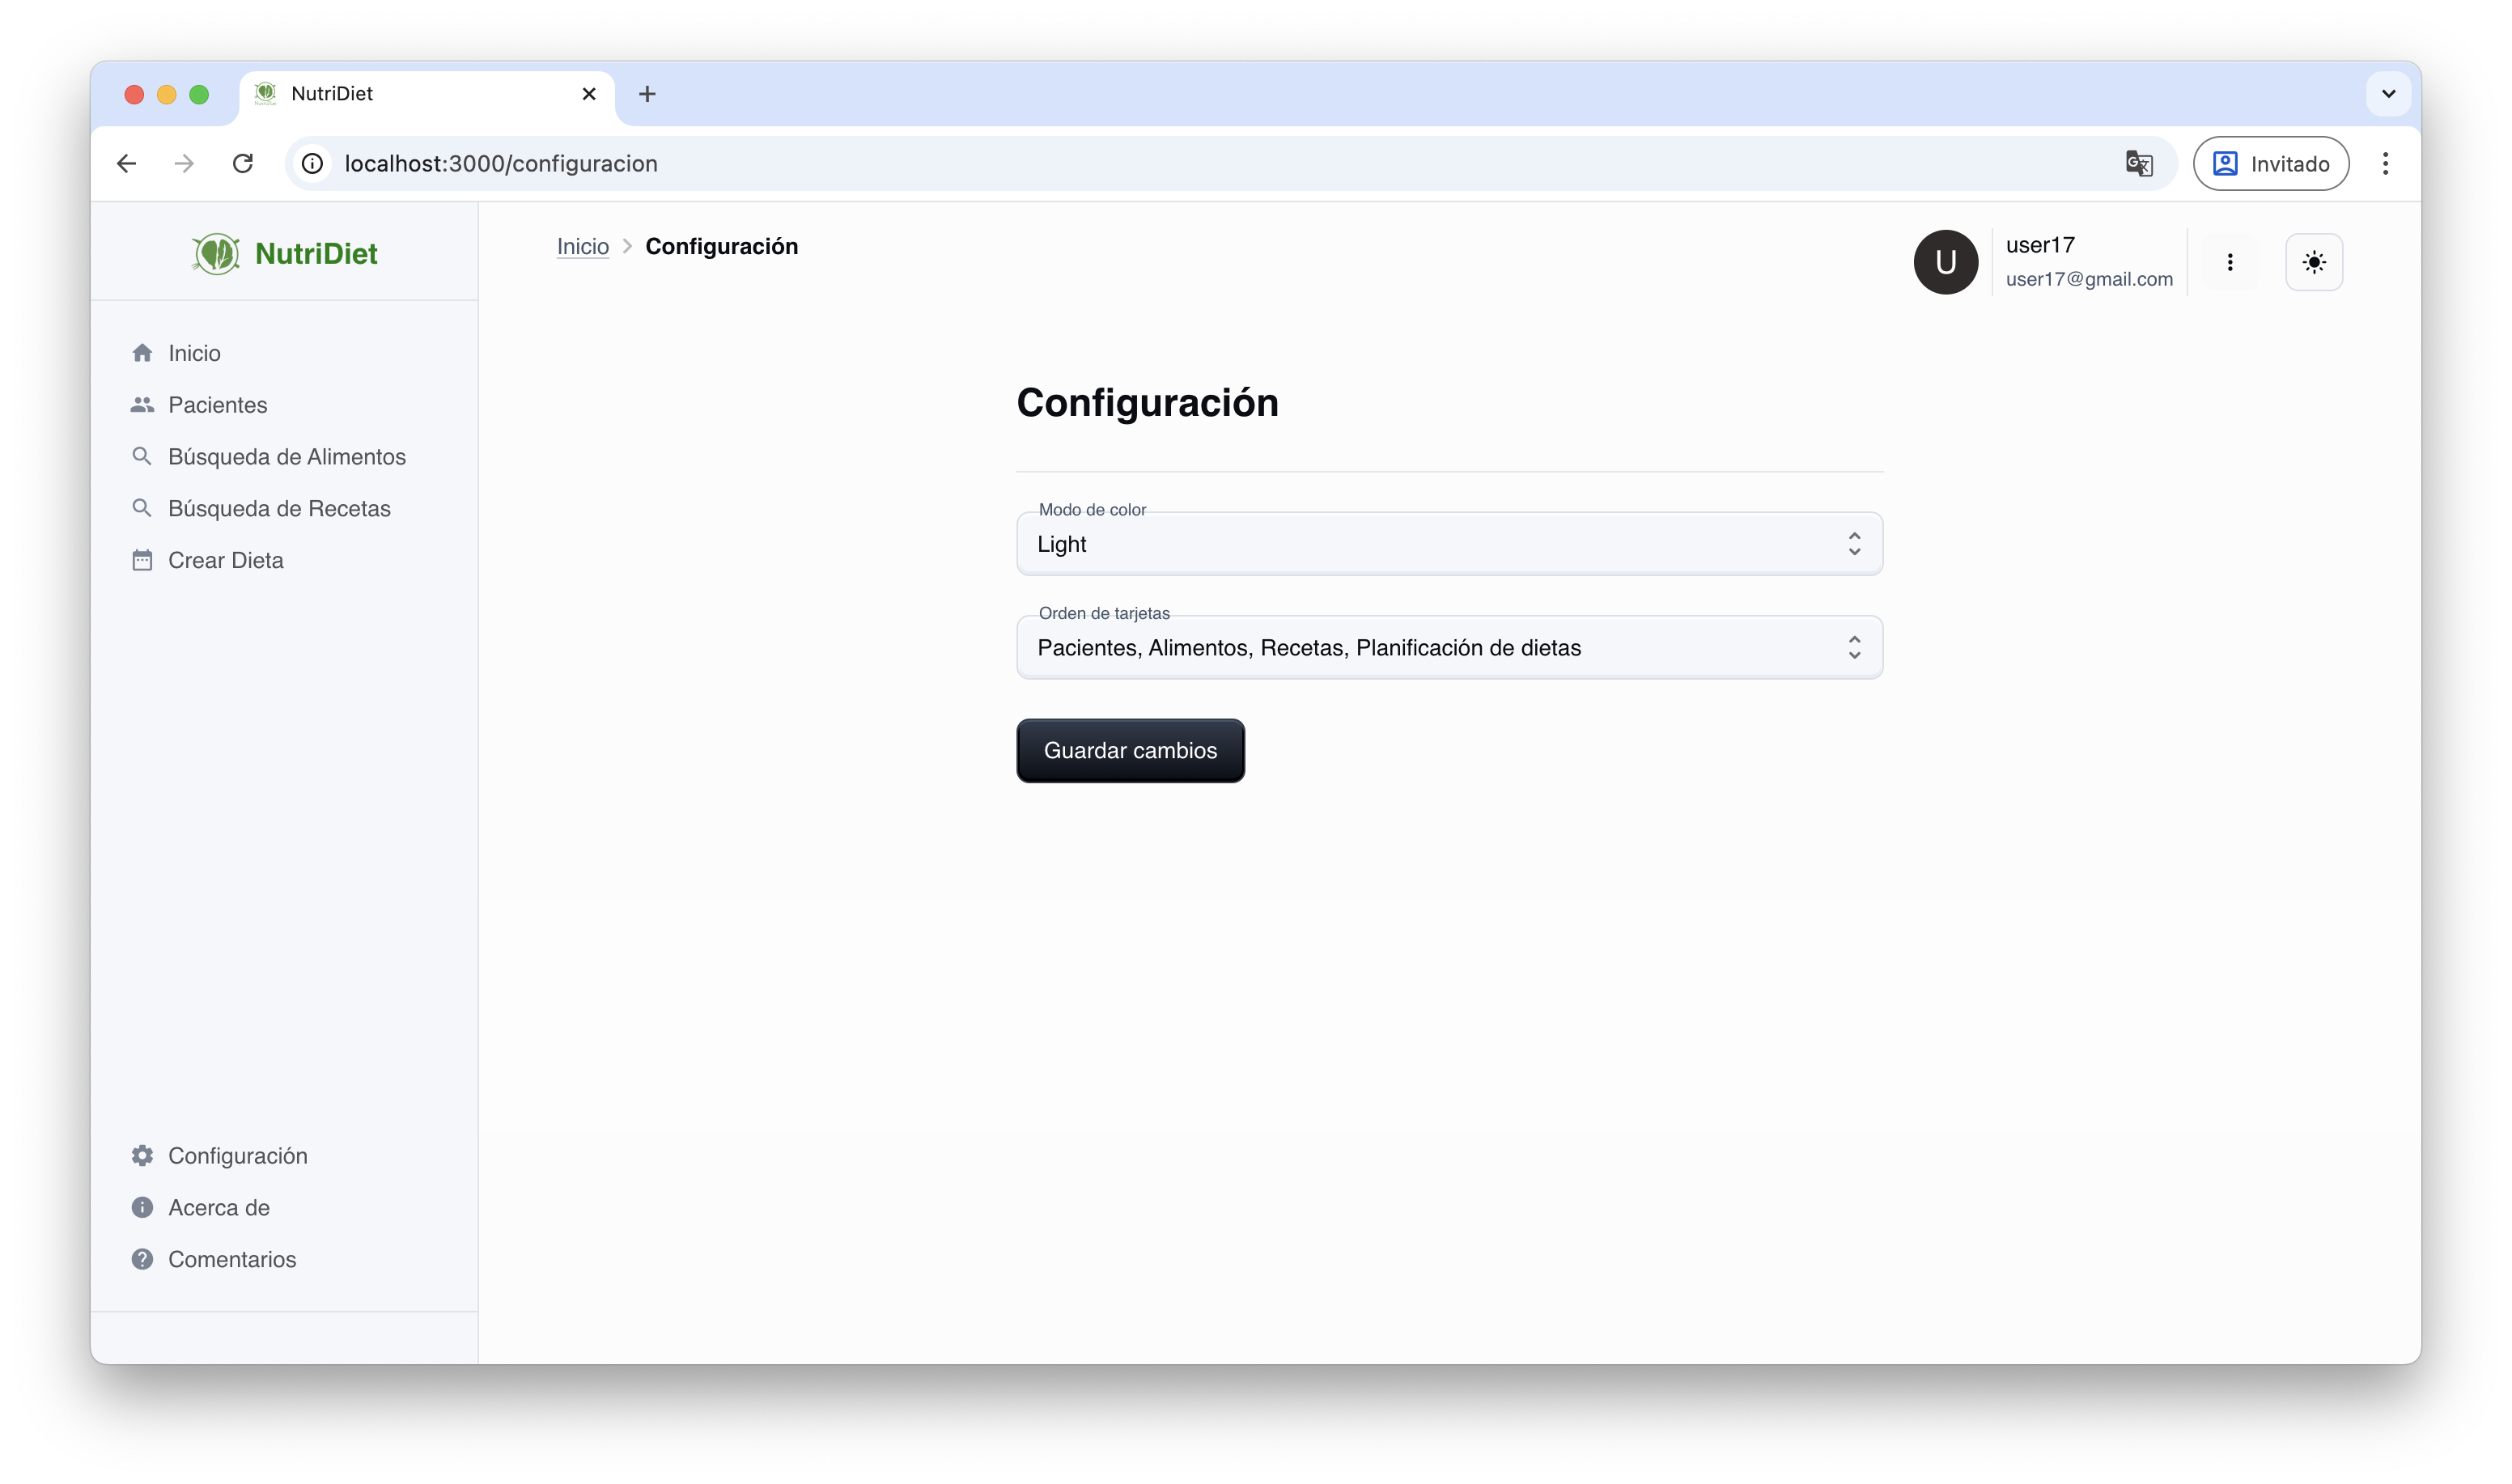
\includegraphics[width=1\linewidth]{Plantilla_TFG_latex//imagenes/Configuracion.png}
    \caption{Pantalla de configuración del sistema}
    \label{fig:pantalla-configuracion}
\end{figure}

\section{Consideraciones finales del capítulo}
En este capítulo proporciona una guía detallada sobre el funcionamiento de cada una de las funcionalidades integradas en el sistema.
Cada módulo ha sido diseñado con un enfoque centrado en la usabilidad y la personalización, como se refleja en opciones como la configuración del sistema o la planificación alimentaria adaptada a cada paciente. 

En conjunto, el sistema cumple con los requisitos establecidos y responde de manera efectiva a las necesidades detectadas durante el análisis, consolidándose como una solución digital integral para la gestión nutricional personalizada. Además, se ha realizado un video de demo funcional donde se puede visualizar el comportamiento del sistema (\url{https://drive.google.com/file/d/10IC1oFVbOKyTe_VdsKLkdpSt9aNQeZIn/view?usp=sharing}).

%
\chapter{Conclusiones y trabajos futuros}\label{capitulo8}
\section{Conclusiones}

El objetivo principal de este Trabajo de Fin de Grado ha sido desarrollar un sistema digital que facilite a los nutricionistas la planificación y gestión de dietas personalizadas para sus pacientes. El sistema se ha construido sobre una arquitectura moderna, compuesta por React en el frontend, FastAPI en el backend y MongoDB como base de datos, con el fin de ofrecer una herramienta práctica que sirva de apoyo en la toma de decisiones nutricionales.

Los resultados obtenidos han sido muy satisfactorios y se han alcanzado de acuerdo con la planificación establecida. El sistema desarrollado es completamente funcional y cubre las necesidades esenciales del proceso: permite registrar y editar pacientes, gestionar recetas, planificar ingestas diarias y estructurar dietas completas. 

Además, se han incorporado funcionalidades útiles como los filtros por categoría y por valores nutricionales, la búsqueda semántica de recetas, sugerencias de recetas y alimentos mediante modelos de lenguaje con embeddings, búsqueda semántica de recetas, la visualización detallada de información nutricional por raciones estándar, caseras o por unidad y la integración de bases de datos especializadas, tanto propias como externas, para respaldar los valores nutricionales y estandarizar los ingredientes utilizados. Este trabajo ha requerido una cuidadosa validación y limpieza de datos, así como la adaptación de estructuras compatibles con el modelo de planificación. También se han implementado mecanismos como la exportación de dietas en formato PDF, el diseño de interfaces interactivas con funcionalidades de arrastrar y soltar, y el control seguro de usuarios mediante autenticación con tokens.

Respecto a los objetivos específicos propuestos, el grado de cumplimiento ha sido el siguiente:

\begin{itemize}
    \item Diseñar una arquitectura modular y escalable: 100\,\% completado. Se ha construido una estructura clara basada en servicios RESTful, documentada en el capítulo correspondiente al implementación. 
    \item Crear una interfaz intuitiva para el usuario profesional: 90\,\% completado. Se han implementado formularios dinámicos, navegación fluida y un sistema de organización mediante arrastrar y soltar (``drag-and-drop''), tal como se refleja en el capítulo de resultados.
    \item Gestionar información nutricional por ración: 80\,\% completado. El sistema permite visualizar datos por raciones y unidades domésticas, aunque aún no admite personalización libre de cantidades.
    \item Planificar ingestas diarias: 100\,\% completado. El sistema permite definir tipos de comidas diarias y asociarlas a días concretos, tal y como se detalla en el apartado de planificación.
    \item Crear y almacenar dietas completas: 100\,\% completado. Las dietas se estructuran en días con sus respectivas ingestas, totalmente vinculadas al paciente correspondiente.
\end{itemize}

Durante el desarrollo de este trabajo he podido aplicar muchos de los conocimientos adquiridos a lo largo del grado. En concreto, asignaturas como Bases de datos distribuidas y Administración de bases de datos han sido clave para diseñar la estructura lógica de almacenamiento y para trabajar con MongoDB, permitiendo optimizar las consultas y organizar de manera eficiente los datos.

A través de lo aprendido en las asignaturas \textit{Diseño y desarrollo de sistemas de información} y\textit{ Programación y diseño orientado a objetos}, he afianzado mis habilidades de análisis de requisitos, diseño funcional, identificación de casos de uso y estructuración modular de un sistema. Estas bases han resultado fundamentales para dar coherencia a la solución propuesta.

También resultó especialmente útil lo aprendido en la asignatura  \textit{Ingeniería de Sistemas de Información}, que me dio una visión clara del ciclo de vida de un sistema informático. Esto me permitió planificar de forma ordenada el proyecto, diferenciando las etapas de diseño, implementación y validación.

En cuanto al desarrollo de la interfaz, los conocimientos de la asignatura \textit{Programación Web} (especialmente JavaScript, HTML y CSS) me proporcionaron la base necesaria para entender la lógica del cliente y construir interfaces usables. Sin embargo, la aplicación se ha desarrollado usando React, una biblioteca que no se abordó en clase y que he aprendido de forma autodidacta a lo largo del TFG. Gracias a ello, he podido implementar componentes reutilizables, gestionar el estado con fluidez y conectar eficientemente el frontend con el backend a través de APIs.

Además de React, también fue necesario aprender por mi cuenta tecnologías y conceptos que no se habían tratado previamente en el grado. Entre ellos destacan el uso de FastAPI, la implementación de autenticación con JWT, la validación de datos con Pydantic, y la gestión de rutas protegidas. Asimismo, integré componentes interactivos como ``drag-and-drop'', mejorando la experiencia de usuario en tareas como la creación de dietas e ingestas.

Desde el punto de vista ético y social, considero que este sistema puede tener un impacto positivo real, ya que promueve hábitos alimentarios saludables y facilita la labor del profesional sanitario en la planificación nutricional personalizada. Tal como se mencionaba en la introducción, actualmente existe una creciente preocupación por el aumento de enfermedades crónicas no transmisibles, como la obesidad, la diabetes tipo 2 y las enfermedades cardiovasculares, muchas de ellas asociadas a una mala alimentación. Ante esta situación, disponer de herramientas digitales que apoyen la toma de decisiones nutricionales de forma más eficiente y personalizada cobra una especial relevancia.

Aunque el sistema ha sido desarrollado inicialmente en un entorno académico y funciona en local, su diseño responde a necesidades reales del ámbito profesional. No se trata solo de una práctica académica, sino de una herramienta con utilidad práctica concreta, tanto en entornos clínicos como educativos. De hecho, está prevista su implementación en el gabinete de nutrición de la universidad, donde servirá de apoyo en actividades docentes (en las prácticas de la asignatura de Principios de Dietética) y en sesiones de atención personalizada (en Aula de Nutrición). Esta aplicación directa refuerza el carácter profesional del trabajo y demuestra su valor más allá.

La herramienta permite a los nutricionistas planificar dietas de forma estructurada y ofrecer recomendaciones personalizadas, ajustadas al perfil nutricional de cada paciente. Supone un avance respecto a los métodos tradicionales, aún muy presentes en la práctica diaria, basados en registros manuales o sistemas poco integrados. Además, se alinea con el Objetivo de Desarrollo Sostenible (ODS) 3: Salud y Bienestar, al facilitar la promoción de estilos de vida más saludables y reforzar el papel preventivo de la alimentación a través de soluciones digitales eficaces.

Finalmente, me gustaría destacar que, a diferencia de otros proyectos realizados durante el grado que fueron en grupo, este TFG ha sido desarrollado de forma completamente individual. Esto ha supuesto una diferencia importante en cuanto a organización, toma de decisiones y resolución de problemas. He tenido que gestionar cada fase por mi cuenta, desde la planificación hasta la implementación técnica y la documentación. Ha sido una experiencia exigente pero muy enriquecedora, que me ha ayudado a mejorar mi autonomía, mi capacidad de adaptación y mi seguridad a la hora de abordar proyectos complejos. Me siento satisfecho con los conocimientos adquiridos y con el resultado alcanzado, y creo que este trabajo representa fielmente mi evolución como estudiante y como futuro profesional.

\section{Trabajos futuros}
Debido a la limitación de tiempo y al alcance definido para esta primera versión, hay múltiples funcionalidades que quedan como propuestas para futuras mejoras del sistema:

\begin{itemize}
    \item Preferencias del paciente y filtros personalizados: 
    Actualmente no se ha incorporado un sistema de preferencias alimentarias específicas por paciente. En versiones futuras se propone implementar un formulario de preferencias que permita registrar alergias, alimentos restringidos, hábitos alimentarios, objetivos dietéticos y preferencias culturales. Estas preferencias podrán usarse como filtros automáticos al sugerir recetas o generar dietas.

    \item Porciones variables y unidades domésticas: 
    En la versión actual, los valores nutricionales están calculados únicamente por ración fija. En el futuro, se prevé permitir que el usuario modifique libremente la cantidad de alimento o elija entre porciones estándar (por ejemplo, “vaso pequeño”, “vaso grande” para líquidos como zumos), ajustando dinámicamente los valores nutricionales mostrados.

    \item Creación de recetas personalizadas por parte del usuario:
    En caso de que un nutricionista o paciente no encuentre recetas adecuadas en la base de datos, se ofrecerá la opción de crear recetas propias seleccionando ingredientes disponibles. Esto permitirá generar dietas incluso en ausencia de recetas predefinidas.

    \item Mejoras en las sugerencias de alimentos: 
    Las sugerencias de alimentos podrían refinarse mediante el análisis de su composición nutricional o su frecuencia de aparición en recetas. Un sistema de recomendación basado en datos permitiría proponer alimentos de manera más inteligente y adaptada a cada contexto.

    \item Despliegue en la nube y apertura al público: 
    Actualmente el sistema funciona en local como herramienta académica. En el futuro, se prevé su despliegue en la nube, con una arquitectura segura y escalable, lo que permitiría su uso por nutricionistas reales y pacientes de forma remota.

    \item Interacción en línea mediante chatbot: 
    Para la versión pública, se propone la integración de un chatbot que facilite la comunicación entre paciente y nutricionista. Este asistente virtual podría responder dudas, guiar en la selección de alimentos y dar recomendaciones nutricionales básicas en tiempo real.

\end{itemize}

En definitiva, aunque el sistema se encuentra funcional en su versión actual y cubre las funcionalidades esenciales, aún presenta margen de mejora para convertirlo como una herramienta profesional completa. El desarrollo realizado hasta el momento proporciona una base sólida sobre la que construir futuras versiones, con un alto potencial de aplicación tanto en contextos académicos como en entornos clínicos.


%
%
%
%
% \nocite{*}
% \bibliography{bibliografia/bibliografia.bib}
% \addcontentsline{toc}{chapter}{Bibliografía}
% \bibliographystyle{miunsrturl}


%
%\appendix
%\input{apendices/manual_usuario/manual_usuario}
%%\input{apendices/paper/paper}
%\input{glosario/entradas_glosario}
% \addcontentsline{toc}{chapter}{Glosario}
% \printglossary
% \chapter*{}
% \thispagestyle{empty}



% \printbibliography[title={Bibliografía}]
\addcontentsline{toc}{chapter}{Bibliografía}


\bibliographystyle{plain}
\bibliography{Plantilla_TFG_latex/bibliografia/bibliografia}
\label{capitulo9}
\clearpage


\end{document}
